\documentclass[twoside]{book}

% Packages required by doxygen
\usepackage{fixltx2e}
\usepackage{calc}
\usepackage{doxygen}
\usepackage[export]{adjustbox} % also loads graphicx
\usepackage{graphicx}
\usepackage[utf8]{inputenc}
\usepackage{makeidx}
\usepackage{multicol}
\usepackage{multirow}
\PassOptionsToPackage{warn}{textcomp}
\usepackage{textcomp}
\usepackage[nointegrals]{wasysym}
\usepackage[table]{xcolor}

% Font selection
\usepackage[T1]{fontenc}
\usepackage[scaled=.90]{helvet}
\usepackage{courier}
\usepackage{amssymb}
\usepackage{sectsty}
\renewcommand{\familydefault}{\sfdefault}
\allsectionsfont{%
  \fontseries{bc}\selectfont%
  \color{darkgray}%
}
\renewcommand{\DoxyLabelFont}{%
  \fontseries{bc}\selectfont%
  \color{darkgray}%
}
\newcommand{\+}{\discretionary{\mbox{\scriptsize$\hookleftarrow$}}{}{}}

% Page & text layout
\usepackage{geometry}
\geometry{%
  a4paper,%
  top=2.5cm,%
  bottom=2.5cm,%
  left=2.5cm,%
  right=2.5cm%
}
\tolerance=750
\hfuzz=15pt
\hbadness=750
\setlength{\emergencystretch}{15pt}
\setlength{\parindent}{0cm}
\setlength{\parskip}{3ex plus 2ex minus 2ex}
\makeatletter
\renewcommand{\paragraph}{%
  \@startsection{paragraph}{4}{0ex}{-1.0ex}{1.0ex}{%
    \normalfont\normalsize\bfseries\SS@parafont%
  }%
}
\renewcommand{\subparagraph}{%
  \@startsection{subparagraph}{5}{0ex}{-1.0ex}{1.0ex}{%
    \normalfont\normalsize\bfseries\SS@subparafont%
  }%
}
\makeatother

% Headers & footers
\usepackage{fancyhdr}
\pagestyle{fancyplain}
\fancyhead[LE]{\fancyplain{}{\bfseries\thepage}}
\fancyhead[CE]{\fancyplain{}{}}
\fancyhead[RE]{\fancyplain{}{\bfseries\leftmark}}
\fancyhead[LO]{\fancyplain{}{\bfseries\rightmark}}
\fancyhead[CO]{\fancyplain{}{}}
\fancyhead[RO]{\fancyplain{}{\bfseries\thepage}}
\fancyfoot[LE]{\fancyplain{}{}}
\fancyfoot[CE]{\fancyplain{}{}}
\fancyfoot[RE]{\fancyplain{}{\bfseries\scriptsize Generated by Doxygen }}
\fancyfoot[LO]{\fancyplain{}{\bfseries\scriptsize Generated by Doxygen }}
\fancyfoot[CO]{\fancyplain{}{}}
\fancyfoot[RO]{\fancyplain{}{}}
\renewcommand{\footrulewidth}{0.4pt}
\renewcommand{\chaptermark}[1]{%
  \markboth{#1}{}%
}
\renewcommand{\sectionmark}[1]{%
  \markright{\thesection\ #1}%
}

% Indices & bibliography
\usepackage{natbib}
\usepackage[titles]{tocloft}
\setcounter{tocdepth}{3}
\setcounter{secnumdepth}{5}
\makeindex

% Hyperlinks (required, but should be loaded last)
\usepackage{ifpdf}
\ifpdf
  \usepackage[pdftex,pagebackref=true]{hyperref}
\else
  \usepackage[ps2pdf,pagebackref=true]{hyperref}
\fi
\hypersetup{%
  colorlinks=true,%
  linkcolor=blue,%
  citecolor=blue,%
  unicode%
}

% Custom commands
\newcommand{\clearemptydoublepage}{%
  \newpage{\pagestyle{empty}\cleardoublepage}%
}

\usepackage{caption}
\captionsetup{labelsep=space,justification=centering,font={bf},singlelinecheck=off,skip=4pt,position=top}

%===== C O N T E N T S =====

\begin{document}

% Titlepage & ToC
\hypersetup{pageanchor=false,
             bookmarksnumbered=true,
             pdfencoding=unicode
            }
\pagenumbering{alph}
\begin{titlepage}
\vspace*{7cm}
\begin{center}%
{\Large P\+R\+O\+J\+E\+T\+\_\+\+S4 }\\
\vspace*{1cm}
{\large Generated by Doxygen 1.8.13}\\
\end{center}
\end{titlepage}
\clearemptydoublepage
\pagenumbering{roman}
\tableofcontents
\clearemptydoublepage
\pagenumbering{arabic}
\hypersetup{pageanchor=true}

%--- Begin generated contents ---
\chapter{P\+R\+O\+J\+E\+T\+\_\+\+S4}
\label{md__r_e_a_d_m_e}
\Hypertarget{md__r_e_a_d_m_e}
Projet L2 S4 
\chapter{Data Structure Index}
\section{Data Structures}
Here are the data structures with brief descriptions\+:\begin{DoxyCompactList}
\item\contentsline{section}{\hyperlink{structblock__s}{block\+\_\+s} }{\pageref{structblock__s}}{}
\item\contentsline{section}{\hyperlink{structfile__s}{file\+\_\+s} }{\pageref{structfile__s}}{}
\item\contentsline{section}{\hyperlink{structinode__s}{inode\+\_\+s} }{\pageref{structinode__s}}{}
\item\contentsline{section}{\hyperlink{structstripe__s}{stripe\+\_\+s} }{\pageref{structstripe__s}}{}
\item\contentsline{section}{\hyperlink{structsuper__block__s}{super\+\_\+block\+\_\+s} }{\pageref{structsuper__block__s}}{}
\item\contentsline{section}{\hyperlink{structvirtual__disk__s}{virtual\+\_\+disk\+\_\+s} }{\pageref{structvirtual__disk__s}}{}
\end{DoxyCompactList}

\chapter{File Index}
\section{File List}
Here is a list of all files with brief descriptions\+:\begin{DoxyCompactList}
\item\contentsline{section}{\hyperlink{cmd__format_8c}{cmd\+\_\+format.\+c} }{\pageref{cmd__format_8c}}{}
\item\contentsline{section}{\hyperlink{cmd__format_8h}{cmd\+\_\+format.\+h} }{\pageref{cmd__format_8h}}{}
\item\contentsline{section}{\hyperlink{couche1_8c}{couche1.\+c} \\*Programme couche1 du raid5 }{\pageref{couche1_8c}}{}
\item\contentsline{section}{\hyperlink{couche1_8h}{couche1.\+h} }{\pageref{couche1_8h}}{}
\item\contentsline{section}{\hyperlink{couche2_8c}{couche2.\+c} \\*Programme couche2 du raid5 }{\pageref{couche2_8c}}{}
\item\contentsline{section}{\hyperlink{couche2_8h}{couche2.\+h} }{\pageref{couche2_8h}}{}
\item\contentsline{section}{\hyperlink{couche3_8c}{couche3.\+c} \\*Programme couche3 du raid5 }{\pageref{couche3_8c}}{}
\item\contentsline{section}{\hyperlink{couche3_8h}{couche3.\+h} }{\pageref{couche3_8h}}{}
\item\contentsline{section}{\hyperlink{raid__defines_8h}{raid\+\_\+defines.\+h} }{\pageref{raid__defines_8h}}{}
\item\contentsline{section}{\hyperlink{trash_8c}{trash.\+c} }{\pageref{trash_8c}}{}
\end{DoxyCompactList}

\chapter{Data Structure Documentation}
\hypertarget{structblock__s}{}\section{block\+\_\+s Struct Reference}
\label{structblock__s}\index{block\+\_\+s@{block\+\_\+s}}


{\ttfamily \#include $<$raid\+\_\+defines.\+h$>$}

\subsection*{Data Fields}
\begin{DoxyCompactItemize}
\item 
\hyperlink{raid__defines_8h_a65f85814a8290f9797005d3b28e7e5fc}{uchar} \hyperlink{structblock__s_aeb657a9749b851021c3ef39acaf7b252}{data} \mbox{[}\hyperlink{raid__defines_8h_ad51ded0bbd705f02f73fc60c0b721ced}{B\+L\+O\+C\+K\+\_\+\+S\+I\+ZE}\mbox{]}
\end{DoxyCompactItemize}


\subsection{Detailed Description}


Definition at line 23 of file raid\+\_\+defines.\+h.



\subsection{Field Documentation}
\mbox{\Hypertarget{structblock__s_aeb657a9749b851021c3ef39acaf7b252}\label{structblock__s_aeb657a9749b851021c3ef39acaf7b252}} 
\index{block\+\_\+s@{block\+\_\+s}!data@{data}}
\index{data@{data}!block\+\_\+s@{block\+\_\+s}}
\subsubsection{\texorpdfstring{data}{data}}
{\footnotesize\ttfamily \hyperlink{raid__defines_8h_a65f85814a8290f9797005d3b28e7e5fc}{uchar} data\mbox{[}\hyperlink{raid__defines_8h_ad51ded0bbd705f02f73fc60c0b721ced}{B\+L\+O\+C\+K\+\_\+\+S\+I\+ZE}\mbox{]}}



Definition at line 24 of file raid\+\_\+defines.\+h.



The documentation for this struct was generated from the following file\+:\begin{DoxyCompactItemize}
\item 
\hyperlink{raid__defines_8h}{raid\+\_\+defines.\+h}\end{DoxyCompactItemize}

\hypertarget{structfile__s}{}\section{file\+\_\+s Struct Reference}
\label{structfile__s}\index{file\+\_\+s@{file\+\_\+s}}


{\ttfamily \#include $<$raid\+\_\+defines.\+h$>$}

\subsection*{Data Fields}
\begin{DoxyCompactItemize}
\item 
\hyperlink{raid__defines_8h_a91ad9478d81a7aaf2593e8d9c3d06a14}{uint} \hyperlink{structfile__s_a22d26304a3b3aca97e6311f6939dd1bf}{size}
\item 
\hyperlink{raid__defines_8h_a65f85814a8290f9797005d3b28e7e5fc}{uchar} \hyperlink{structfile__s_a5f05d979f42df3908fb0f491f6c65256}{data} \mbox{[}\hyperlink{raid__defines_8h_a649ad5274d988d17a275a3cead056746}{M\+A\+X\+\_\+\+F\+I\+L\+E\+\_\+\+S\+I\+ZE}\mbox{]}
\end{DoxyCompactItemize}


\subsection{Detailed Description}


Definition at line 62 of file raid\+\_\+defines.\+h.



\subsection{Field Documentation}
\mbox{\Hypertarget{structfile__s_a5f05d979f42df3908fb0f491f6c65256}\label{structfile__s_a5f05d979f42df3908fb0f491f6c65256}} 
\index{file\+\_\+s@{file\+\_\+s}!data@{data}}
\index{data@{data}!file\+\_\+s@{file\+\_\+s}}
\subsubsection{\texorpdfstring{data}{data}}
{\footnotesize\ttfamily \hyperlink{raid__defines_8h_a65f85814a8290f9797005d3b28e7e5fc}{uchar} data\mbox{[}\hyperlink{raid__defines_8h_a649ad5274d988d17a275a3cead056746}{M\+A\+X\+\_\+\+F\+I\+L\+E\+\_\+\+S\+I\+ZE}\mbox{]}}



Definition at line 64 of file raid\+\_\+defines.\+h.

\mbox{\Hypertarget{structfile__s_a22d26304a3b3aca97e6311f6939dd1bf}\label{structfile__s_a22d26304a3b3aca97e6311f6939dd1bf}} 
\index{file\+\_\+s@{file\+\_\+s}!size@{size}}
\index{size@{size}!file\+\_\+s@{file\+\_\+s}}
\subsubsection{\texorpdfstring{size}{size}}
{\footnotesize\ttfamily \hyperlink{raid__defines_8h_a91ad9478d81a7aaf2593e8d9c3d06a14}{uint} size}



Definition at line 63 of file raid\+\_\+defines.\+h.



The documentation for this struct was generated from the following file\+:\begin{DoxyCompactItemize}
\item 
\hyperlink{raid__defines_8h}{raid\+\_\+defines.\+h}\end{DoxyCompactItemize}

\hypertarget{structinode__s}{}\section{inode\+\_\+s Struct Reference}
\label{structinode__s}\index{inode\+\_\+s@{inode\+\_\+s}}


{\ttfamily \#include $<$raid\+\_\+defines.\+h$>$}

\subsection*{Data Fields}
\begin{DoxyCompactItemize}
\item 
char \hyperlink{structinode__s_a620f1f08587e3ad63c74a9fb90bb9be8}{filename} \mbox{[}\hyperlink{raid__defines_8h_a24c1405225e4ce27b24bcf4f32f4ff0e}{F\+I\+L\+E\+N\+A\+M\+E\+\_\+\+M\+A\+X\+\_\+\+S\+I\+ZE}\mbox{]}
\item 
\hyperlink{raid__defines_8h_a91ad9478d81a7aaf2593e8d9c3d06a14}{uint} \hyperlink{structinode__s_a22d26304a3b3aca97e6311f6939dd1bf}{size}
\item 
\hyperlink{raid__defines_8h_a91ad9478d81a7aaf2593e8d9c3d06a14}{uint} \hyperlink{structinode__s_afe7beb909cfc74858acbb6c26d5d0e00}{nblock}
\item 
\hyperlink{raid__defines_8h_a91ad9478d81a7aaf2593e8d9c3d06a14}{uint} \hyperlink{structinode__s_a4513cc558a2d925cd5b3023ea6b3ba62}{first\+\_\+byte}
\end{DoxyCompactItemize}


\subsection{Detailed Description}


Definition at line 28 of file raid\+\_\+defines.\+h.



\subsection{Field Documentation}
\mbox{\Hypertarget{structinode__s_a620f1f08587e3ad63c74a9fb90bb9be8}\label{structinode__s_a620f1f08587e3ad63c74a9fb90bb9be8}} 
\index{inode\+\_\+s@{inode\+\_\+s}!filename@{filename}}
\index{filename@{filename}!inode\+\_\+s@{inode\+\_\+s}}
\subsubsection{\texorpdfstring{filename}{filename}}
{\footnotesize\ttfamily char filename\mbox{[}\hyperlink{raid__defines_8h_a24c1405225e4ce27b24bcf4f32f4ff0e}{F\+I\+L\+E\+N\+A\+M\+E\+\_\+\+M\+A\+X\+\_\+\+S\+I\+ZE}\mbox{]}}



Definition at line 29 of file raid\+\_\+defines.\+h.

\mbox{\Hypertarget{structinode__s_a4513cc558a2d925cd5b3023ea6b3ba62}\label{structinode__s_a4513cc558a2d925cd5b3023ea6b3ba62}} 
\index{inode\+\_\+s@{inode\+\_\+s}!first\+\_\+byte@{first\+\_\+byte}}
\index{first\+\_\+byte@{first\+\_\+byte}!inode\+\_\+s@{inode\+\_\+s}}
\subsubsection{\texorpdfstring{first\+\_\+byte}{first\_byte}}
{\footnotesize\ttfamily \hyperlink{raid__defines_8h_a91ad9478d81a7aaf2593e8d9c3d06a14}{uint} first\+\_\+byte}



Definition at line 32 of file raid\+\_\+defines.\+h.

\mbox{\Hypertarget{structinode__s_afe7beb909cfc74858acbb6c26d5d0e00}\label{structinode__s_afe7beb909cfc74858acbb6c26d5d0e00}} 
\index{inode\+\_\+s@{inode\+\_\+s}!nblock@{nblock}}
\index{nblock@{nblock}!inode\+\_\+s@{inode\+\_\+s}}
\subsubsection{\texorpdfstring{nblock}{nblock}}
{\footnotesize\ttfamily \hyperlink{raid__defines_8h_a91ad9478d81a7aaf2593e8d9c3d06a14}{uint} nblock}



Definition at line 31 of file raid\+\_\+defines.\+h.

\mbox{\Hypertarget{structinode__s_a22d26304a3b3aca97e6311f6939dd1bf}\label{structinode__s_a22d26304a3b3aca97e6311f6939dd1bf}} 
\index{inode\+\_\+s@{inode\+\_\+s}!size@{size}}
\index{size@{size}!inode\+\_\+s@{inode\+\_\+s}}
\subsubsection{\texorpdfstring{size}{size}}
{\footnotesize\ttfamily \hyperlink{raid__defines_8h_a91ad9478d81a7aaf2593e8d9c3d06a14}{uint} size}



Definition at line 30 of file raid\+\_\+defines.\+h.



The documentation for this struct was generated from the following file\+:\begin{DoxyCompactItemize}
\item 
\hyperlink{raid__defines_8h}{raid\+\_\+defines.\+h}\end{DoxyCompactItemize}

\hypertarget{structstripe__s}{}\section{stripe\+\_\+s Struct Reference}
\label{structstripe__s}\index{stripe\+\_\+s@{stripe\+\_\+s}}


{\ttfamily \#include $<$raid\+\_\+defines.\+h$>$}



Collaboration diagram for stripe\+\_\+s\+:
\nopagebreak
\begin{figure}[H]
\begin{center}
\leavevmode
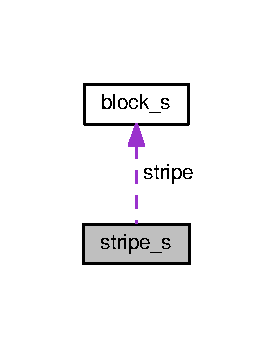
\includegraphics[width=134pt]{structstripe__s__coll__graph}
\end{center}
\end{figure}
\subsection*{Data Fields}
\begin{DoxyCompactItemize}
\item 
int \hyperlink{structstripe__s_a076c8e8b7f7acccc46cd356bd8776b26}{nblocks}
\item 
\hyperlink{raid__defines_8h_a9497df9c1d65b018066a9760da7be4e6}{block\+\_\+t} $\ast$ \hyperlink{structstripe__s_a16ff6d534dd4944c7fc544e4247e5ff1}{stripe}
\end{DoxyCompactItemize}


\subsection{Detailed Description}


Definition at line 56 of file raid\+\_\+defines.\+h.



\subsection{Field Documentation}
\mbox{\Hypertarget{structstripe__s_a076c8e8b7f7acccc46cd356bd8776b26}\label{structstripe__s_a076c8e8b7f7acccc46cd356bd8776b26}} 
\index{stripe\+\_\+s@{stripe\+\_\+s}!nblocks@{nblocks}}
\index{nblocks@{nblocks}!stripe\+\_\+s@{stripe\+\_\+s}}
\subsubsection{\texorpdfstring{nblocks}{nblocks}}
{\footnotesize\ttfamily int nblocks}



Definition at line 58 of file raid\+\_\+defines.\+h.

\mbox{\Hypertarget{structstripe__s_a16ff6d534dd4944c7fc544e4247e5ff1}\label{structstripe__s_a16ff6d534dd4944c7fc544e4247e5ff1}} 
\index{stripe\+\_\+s@{stripe\+\_\+s}!stripe@{stripe}}
\index{stripe@{stripe}!stripe\+\_\+s@{stripe\+\_\+s}}
\subsubsection{\texorpdfstring{stripe}{stripe}}
{\footnotesize\ttfamily \hyperlink{raid__defines_8h_a9497df9c1d65b018066a9760da7be4e6}{block\+\_\+t}$\ast$ stripe}



Definition at line 59 of file raid\+\_\+defines.\+h.



The documentation for this struct was generated from the following file\+:\begin{DoxyCompactItemize}
\item 
\hyperlink{raid__defines_8h}{raid\+\_\+defines.\+h}\end{DoxyCompactItemize}

\hypertarget{structsuper__block__s}{}\section{super\+\_\+block\+\_\+s Struct Reference}
\label{structsuper__block__s}\index{super\+\_\+block\+\_\+s@{super\+\_\+block\+\_\+s}}


{\ttfamily \#include $<$raid\+\_\+defines.\+h$>$}

\subsection*{Data Fields}
\begin{DoxyCompactItemize}
\item 
enum \hyperlink{raid__defines_8h_a7a2279e0841d50aa8e976d3bb0eb3a6e}{raid} \hyperlink{structsuper__block__s_a531486677d7c826dad518c717abcd4ed}{raid\+\_\+type}
\item 
\hyperlink{raid__defines_8h_a91ad9478d81a7aaf2593e8d9c3d06a14}{uint} \hyperlink{structsuper__block__s_a471e84cd18cb41ccc12b4e188c003694}{nb\+\_\+blocks\+\_\+used}
\item 
\hyperlink{raid__defines_8h_a91ad9478d81a7aaf2593e8d9c3d06a14}{uint} \hyperlink{structsuper__block__s_a8fcb4bf17f15b15d1e43aec5a7b22f3f}{first\+\_\+free\+\_\+byte}
\end{DoxyCompactItemize}


\subsection{Detailed Description}


Definition at line 39 of file raid\+\_\+defines.\+h.



\subsection{Field Documentation}
\mbox{\Hypertarget{structsuper__block__s_a8fcb4bf17f15b15d1e43aec5a7b22f3f}\label{structsuper__block__s_a8fcb4bf17f15b15d1e43aec5a7b22f3f}} 
\index{super\+\_\+block\+\_\+s@{super\+\_\+block\+\_\+s}!first\+\_\+free\+\_\+byte@{first\+\_\+free\+\_\+byte}}
\index{first\+\_\+free\+\_\+byte@{first\+\_\+free\+\_\+byte}!super\+\_\+block\+\_\+s@{super\+\_\+block\+\_\+s}}
\subsubsection{\texorpdfstring{first\+\_\+free\+\_\+byte}{first\_free\_byte}}
{\footnotesize\ttfamily \hyperlink{raid__defines_8h_a91ad9478d81a7aaf2593e8d9c3d06a14}{uint} first\+\_\+free\+\_\+byte}



Definition at line 42 of file raid\+\_\+defines.\+h.

\mbox{\Hypertarget{structsuper__block__s_a471e84cd18cb41ccc12b4e188c003694}\label{structsuper__block__s_a471e84cd18cb41ccc12b4e188c003694}} 
\index{super\+\_\+block\+\_\+s@{super\+\_\+block\+\_\+s}!nb\+\_\+blocks\+\_\+used@{nb\+\_\+blocks\+\_\+used}}
\index{nb\+\_\+blocks\+\_\+used@{nb\+\_\+blocks\+\_\+used}!super\+\_\+block\+\_\+s@{super\+\_\+block\+\_\+s}}
\subsubsection{\texorpdfstring{nb\+\_\+blocks\+\_\+used}{nb\_blocks\_used}}
{\footnotesize\ttfamily \hyperlink{raid__defines_8h_a91ad9478d81a7aaf2593e8d9c3d06a14}{uint} nb\+\_\+blocks\+\_\+used}



Definition at line 41 of file raid\+\_\+defines.\+h.

\mbox{\Hypertarget{structsuper__block__s_a531486677d7c826dad518c717abcd4ed}\label{structsuper__block__s_a531486677d7c826dad518c717abcd4ed}} 
\index{super\+\_\+block\+\_\+s@{super\+\_\+block\+\_\+s}!raid\+\_\+type@{raid\+\_\+type}}
\index{raid\+\_\+type@{raid\+\_\+type}!super\+\_\+block\+\_\+s@{super\+\_\+block\+\_\+s}}
\subsubsection{\texorpdfstring{raid\+\_\+type}{raid\_type}}
{\footnotesize\ttfamily enum \hyperlink{raid__defines_8h_a7a2279e0841d50aa8e976d3bb0eb3a6e}{raid} raid\+\_\+type}



Definition at line 40 of file raid\+\_\+defines.\+h.



The documentation for this struct was generated from the following file\+:\begin{DoxyCompactItemize}
\item 
\hyperlink{raid__defines_8h}{raid\+\_\+defines.\+h}\end{DoxyCompactItemize}

\hypertarget{structvirtual__disk__s}{}\section{virtual\+\_\+disk\+\_\+s Struct Reference}
\label{structvirtual__disk__s}\index{virtual\+\_\+disk\+\_\+s@{virtual\+\_\+disk\+\_\+s}}


{\ttfamily \#include $<$raid\+\_\+defines.\+h$>$}



Collaboration diagram for virtual\+\_\+disk\+\_\+s\+:
\nopagebreak
\begin{figure}[H]
\begin{center}
\leavevmode
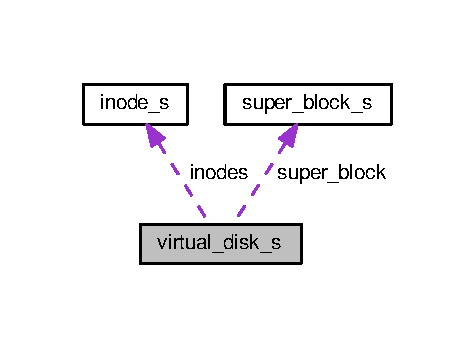
\includegraphics[width=228pt]{structvirtual__disk__s__coll__graph}
\end{center}
\end{figure}
\subsection*{Data Fields}
\begin{DoxyCompactItemize}
\item 
int \hyperlink{structvirtual__disk__s_a465d502eed9840aad6ec9f3a5a5d844c}{number\+\_\+of\+\_\+files}
\item 
\hyperlink{raid__defines_8h_a5b2244b463782d93e6dfc058790cb9eb}{super\+\_\+block\+\_\+t} \hyperlink{structvirtual__disk__s_a32d9616143f7763451383a6c626038ca}{super\+\_\+block}
\item 
\hyperlink{raid__defines_8h_a5521b19dad3852291fc7d603382e6b99}{inode\+\_\+table\+\_\+t} \hyperlink{structvirtual__disk__s_a1bcc97bff109cd0065249a564a71d5c8}{inodes}
\item 
int \hyperlink{structvirtual__disk__s_a879b20de8088f4342835d5fb3feb1141}{ndisk}
\item 
enum \hyperlink{raid__defines_8h_a7a2279e0841d50aa8e976d3bb0eb3a6e}{raid} \hyperlink{structvirtual__disk__s_a207dd070642dde7ad48f8bb8b622f893}{raidmode}
\item 
F\+I\+LE $\ast$$\ast$ \hyperlink{structvirtual__disk__s_abed1c5c15dd8f784e7198b79f8973863}{storage}
\end{DoxyCompactItemize}


\subsection{Detailed Description}


Definition at line 46 of file raid\+\_\+defines.\+h.



\subsection{Field Documentation}
\mbox{\Hypertarget{structvirtual__disk__s_a1bcc97bff109cd0065249a564a71d5c8}\label{structvirtual__disk__s_a1bcc97bff109cd0065249a564a71d5c8}} 
\index{virtual\+\_\+disk\+\_\+s@{virtual\+\_\+disk\+\_\+s}!inodes@{inodes}}
\index{inodes@{inodes}!virtual\+\_\+disk\+\_\+s@{virtual\+\_\+disk\+\_\+s}}
\subsubsection{\texorpdfstring{inodes}{inodes}}
{\footnotesize\ttfamily \hyperlink{raid__defines_8h_a5521b19dad3852291fc7d603382e6b99}{inode\+\_\+table\+\_\+t} inodes}



Definition at line 49 of file raid\+\_\+defines.\+h.

\mbox{\Hypertarget{structvirtual__disk__s_a879b20de8088f4342835d5fb3feb1141}\label{structvirtual__disk__s_a879b20de8088f4342835d5fb3feb1141}} 
\index{virtual\+\_\+disk\+\_\+s@{virtual\+\_\+disk\+\_\+s}!ndisk@{ndisk}}
\index{ndisk@{ndisk}!virtual\+\_\+disk\+\_\+s@{virtual\+\_\+disk\+\_\+s}}
\subsubsection{\texorpdfstring{ndisk}{ndisk}}
{\footnotesize\ttfamily int ndisk}



Definition at line 50 of file raid\+\_\+defines.\+h.

\mbox{\Hypertarget{structvirtual__disk__s_a465d502eed9840aad6ec9f3a5a5d844c}\label{structvirtual__disk__s_a465d502eed9840aad6ec9f3a5a5d844c}} 
\index{virtual\+\_\+disk\+\_\+s@{virtual\+\_\+disk\+\_\+s}!number\+\_\+of\+\_\+files@{number\+\_\+of\+\_\+files}}
\index{number\+\_\+of\+\_\+files@{number\+\_\+of\+\_\+files}!virtual\+\_\+disk\+\_\+s@{virtual\+\_\+disk\+\_\+s}}
\subsubsection{\texorpdfstring{number\+\_\+of\+\_\+files}{number\_of\_files}}
{\footnotesize\ttfamily int number\+\_\+of\+\_\+files}



Definition at line 47 of file raid\+\_\+defines.\+h.

\mbox{\Hypertarget{structvirtual__disk__s_a207dd070642dde7ad48f8bb8b622f893}\label{structvirtual__disk__s_a207dd070642dde7ad48f8bb8b622f893}} 
\index{virtual\+\_\+disk\+\_\+s@{virtual\+\_\+disk\+\_\+s}!raidmode@{raidmode}}
\index{raidmode@{raidmode}!virtual\+\_\+disk\+\_\+s@{virtual\+\_\+disk\+\_\+s}}
\subsubsection{\texorpdfstring{raidmode}{raidmode}}
{\footnotesize\ttfamily enum \hyperlink{raid__defines_8h_a7a2279e0841d50aa8e976d3bb0eb3a6e}{raid} raidmode}



Definition at line 51 of file raid\+\_\+defines.\+h.

\mbox{\Hypertarget{structvirtual__disk__s_abed1c5c15dd8f784e7198b79f8973863}\label{structvirtual__disk__s_abed1c5c15dd8f784e7198b79f8973863}} 
\index{virtual\+\_\+disk\+\_\+s@{virtual\+\_\+disk\+\_\+s}!storage@{storage}}
\index{storage@{storage}!virtual\+\_\+disk\+\_\+s@{virtual\+\_\+disk\+\_\+s}}
\subsubsection{\texorpdfstring{storage}{storage}}
{\footnotesize\ttfamily F\+I\+LE$\ast$$\ast$ storage}



Definition at line 52 of file raid\+\_\+defines.\+h.

\mbox{\Hypertarget{structvirtual__disk__s_a32d9616143f7763451383a6c626038ca}\label{structvirtual__disk__s_a32d9616143f7763451383a6c626038ca}} 
\index{virtual\+\_\+disk\+\_\+s@{virtual\+\_\+disk\+\_\+s}!super\+\_\+block@{super\+\_\+block}}
\index{super\+\_\+block@{super\+\_\+block}!virtual\+\_\+disk\+\_\+s@{virtual\+\_\+disk\+\_\+s}}
\subsubsection{\texorpdfstring{super\+\_\+block}{super\_block}}
{\footnotesize\ttfamily \hyperlink{raid__defines_8h_a5b2244b463782d93e6dfc058790cb9eb}{super\+\_\+block\+\_\+t} super\+\_\+block}



Definition at line 48 of file raid\+\_\+defines.\+h.



The documentation for this struct was generated from the following file\+:\begin{DoxyCompactItemize}
\item 
\hyperlink{raid__defines_8h}{raid\+\_\+defines.\+h}\end{DoxyCompactItemize}

\chapter{File Documentation}
\hypertarget{cmd__format_8c}{}\section{cmd\+\_\+format.\+c File Reference}
\label{cmd__format_8c}\index{cmd\+\_\+format.\+c@{cmd\+\_\+format.\+c}}
{\ttfamily \#include $<$stdio.\+h$>$}\newline
{\ttfamily \#include $<$stdlib.\+h$>$}\newline
{\ttfamily \#include $<$string.\+h$>$}\newline
{\ttfamily \#include $<$assert.\+h$>$}\newline
Include dependency graph for cmd\+\_\+format.\+c\+:
\nopagebreak
\begin{figure}[H]
\begin{center}
\leavevmode
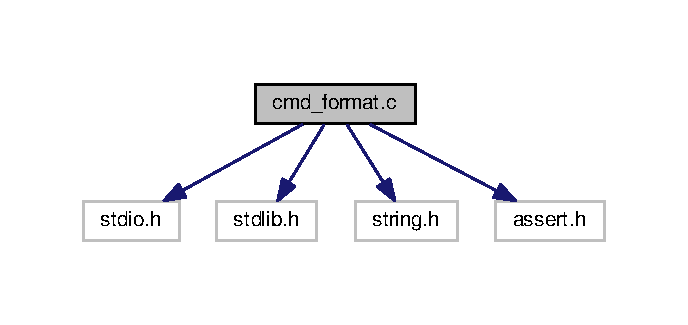
\includegraphics[width=330pt]{cmd__format_8c__incl}
\end{center}
\end{figure}
\subsection*{Functions}
\begin{DoxyCompactItemize}
\item 
void \hyperlink{cmd__format_8c_a98689d86fdfbc9de409689e8f44240d2}{format} (char $\ast$dirname, int size, int diskid)
\item 
int \hyperlink{cmd__format_8c_a3c04138a5bfe5d72780bb7e82a18e627}{main} (int argc, char $\ast$$\ast$argv)
\end{DoxyCompactItemize}


\subsection{Function Documentation}
\mbox{\Hypertarget{cmd__format_8c_a98689d86fdfbc9de409689e8f44240d2}\label{cmd__format_8c_a98689d86fdfbc9de409689e8f44240d2}} 
\index{cmd\+\_\+format.\+c@{cmd\+\_\+format.\+c}!format@{format}}
\index{format@{format}!cmd\+\_\+format.\+c@{cmd\+\_\+format.\+c}}
\subsubsection{\texorpdfstring{format()}{format()}}
{\footnotesize\ttfamily void format (\begin{DoxyParamCaption}\item[{char $\ast$}]{dirname,  }\item[{int}]{size,  }\item[{int}]{diskid }\end{DoxyParamCaption})}



Definition at line 10 of file cmd\+\_\+format.\+c.

Here is the caller graph for this function\+:
\nopagebreak
\begin{figure}[H]
\begin{center}
\leavevmode
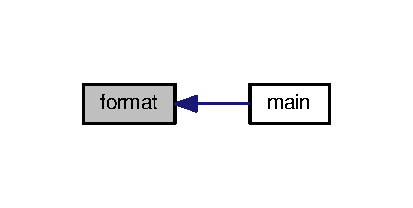
\includegraphics[width=198pt]{cmd__format_8c_a98689d86fdfbc9de409689e8f44240d2_icgraph}
\end{center}
\end{figure}
\mbox{\Hypertarget{cmd__format_8c_a3c04138a5bfe5d72780bb7e82a18e627}\label{cmd__format_8c_a3c04138a5bfe5d72780bb7e82a18e627}} 
\index{cmd\+\_\+format.\+c@{cmd\+\_\+format.\+c}!main@{main}}
\index{main@{main}!cmd\+\_\+format.\+c@{cmd\+\_\+format.\+c}}
\subsubsection{\texorpdfstring{main()}{main()}}
{\footnotesize\ttfamily int main (\begin{DoxyParamCaption}\item[{int}]{argc,  }\item[{char $\ast$$\ast$}]{argv }\end{DoxyParamCaption})}

command nom\+\_\+repertoire nb\+\_\+disks taille\+\_\+fichier (octets) 

Definition at line 24 of file cmd\+\_\+format.\+c.

Here is the call graph for this function\+:
\nopagebreak
\begin{figure}[H]
\begin{center}
\leavevmode
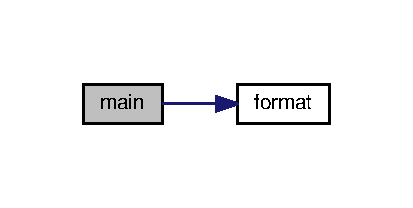
\includegraphics[width=198pt]{cmd__format_8c_a3c04138a5bfe5d72780bb7e82a18e627_cgraph}
\end{center}
\end{figure}

\hypertarget{cmd__format_8h}{}\section{cmd\+\_\+format.\+h File Reference}
\label{cmd__format_8h}\index{cmd\+\_\+format.\+h@{cmd\+\_\+format.\+h}}

\hypertarget{couche1_8c}{}\section{couche1.\+c File Reference}
\label{couche1_8c}\index{couche1.\+c@{couche1.\+c}}


Programme couche1 du raid5.  


{\ttfamily \#include $<$stdio.\+h$>$}\newline
{\ttfamily \#include $<$stdlib.\+h$>$}\newline
{\ttfamily \#include \char`\"{}raid\+\_\+defines.\+h\char`\"{}}\newline
{\ttfamily \#include \char`\"{}couche1.\+h\char`\"{}}\newline
{\ttfamily \#include $<$string.\+h$>$}\newline
{\ttfamily \#include $<$fts.\+h$>$}\newline
{\ttfamily \#include $<$errno.\+h$>$}\newline
{\ttfamily \#include $<$time.\+h$>$}\newline
{\ttfamily \#include $<$stdbool.\+h$>$}\newline
Include dependency graph for couche1.\+c\+:
\nopagebreak
\begin{figure}[H]
\begin{center}
\leavevmode
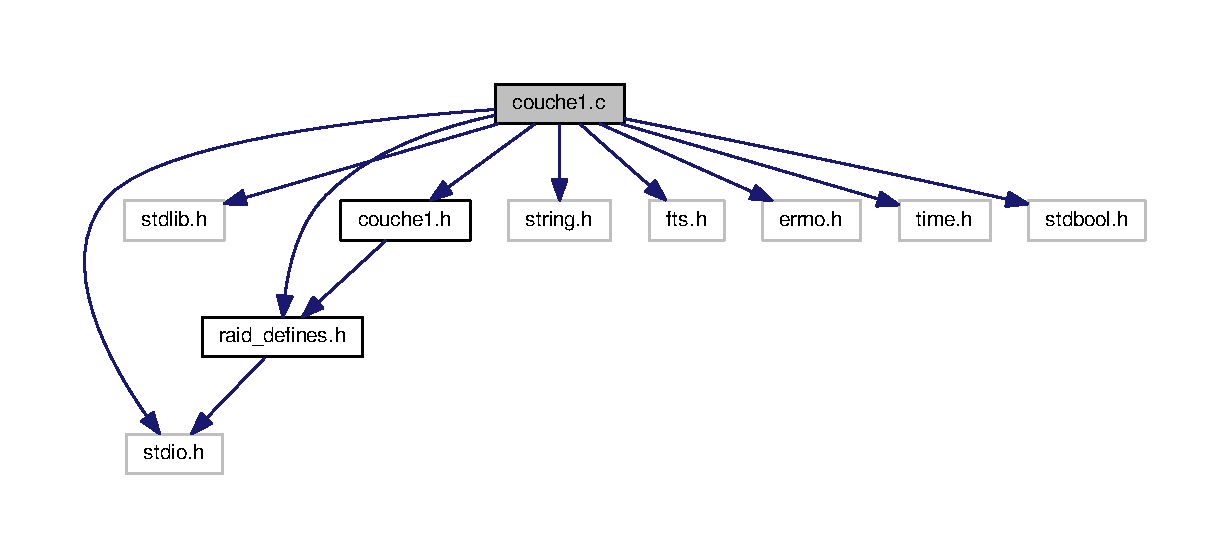
\includegraphics[width=350pt]{couche1_8c__incl}
\end{center}
\end{figure}
\subsection*{Functions}
\begin{DoxyCompactItemize}
\item 
void \hyperlink{couche1_8c_a4479ca3bf5ef9da255dc34dd3b954b04}{add\+\_\+fin\+Chemin} (const char $\ast$repertoire, char $\ast$nom\+Disque, size\+\_\+t length\+Rep)
\begin{DoxyCompactList}\small\item\em Copie la chaine \char`\"{}repertoire\char`\"{} dans nom\+Disque en y ajoutant \char`\"{}/d0\textbackslash{}0\char`\"{}. \end{DoxyCompactList}\item 
void \hyperlink{couche1_8c_a745e214ead4cfa64503c1be97c30d25a}{init\+\_\+disk\+\_\+raid5} (const char $\ast$repertoire, \hyperlink{raid__defines_8h_ab22cb9a2c3c081d95bd06c65d6716686}{virtual\+\_\+disk\+\_\+t} $\ast$\hyperlink{trash_8c_aa32bee7663041ae13a36afeae68a3f14}{r5\+Disk})
\begin{DoxyCompactList}\small\item\em Initialise la variable globale r5\+Disk. \end{DoxyCompactList}\item 
void \hyperlink{couche1_8c_a0f31c284e3b9461448ae2c5393a4c53f}{turn\+\_\+off\+\_\+disk\+\_\+raid5} (\hyperlink{raid__defines_8h_ab22cb9a2c3c081d95bd06c65d6716686}{virtual\+\_\+disk\+\_\+t} $\ast$\hyperlink{trash_8c_aa32bee7663041ae13a36afeae68a3f14}{r5\+Disk})
\begin{DoxyCompactList}\small\item\em Ferme les fichiers ouverts et sauvegarde le super block? \end{DoxyCompactList}\item 
void \hyperlink{couche1_8c_a988f68f7bebc679f512c8eadaa391f16}{info\+\_\+disque} (\hyperlink{raid__defines_8h_ab22cb9a2c3c081d95bd06c65d6716686}{virtual\+\_\+disk\+\_\+t} $\ast$\hyperlink{trash_8c_aa32bee7663041ae13a36afeae68a3f14}{r5\+Disk})
\begin{DoxyCompactList}\small\item\em Affiche des infos sur les disques ouverts. \end{DoxyCompactList}\item 
int \hyperlink{couche1_8c_a9cd7d6dccecc07ca1b67fd05c7928ee3}{compute\+\_\+nblock} (int n)
\begin{DoxyCompactList}\small\item\em calcule le nombre de blocs pour coder \char`\"{}n\char`\"{} octets \end{DoxyCompactList}\item 
void \hyperlink{couche1_8c_adb4607cf11ffed5c89fc0f4682bf6079}{write\+\_\+block} (\hyperlink{raid__defines_8h_ab22cb9a2c3c081d95bd06c65d6716686}{virtual\+\_\+disk\+\_\+t} $\ast$R\+A\+I\+D5, \hyperlink{raid__defines_8h_a9497df9c1d65b018066a9760da7be4e6}{block\+\_\+t} $\ast$entrant, \hyperlink{raid__defines_8h_a91ad9478d81a7aaf2593e8d9c3d06a14}{uint} pos, int id\+Disk)
\begin{DoxyCompactList}\small\item\em Ecrit un bloc à la position pos sur le disque. \end{DoxyCompactList}\item 
int \hyperlink{couche1_8c_a4ba30a1143e543d465725eb0f151c6a2}{read\+\_\+block} (\hyperlink{raid__defines_8h_ab22cb9a2c3c081d95bd06c65d6716686}{virtual\+\_\+disk\+\_\+t} $\ast$R\+A\+I\+D5, \hyperlink{raid__defines_8h_a9497df9c1d65b018066a9760da7be4e6}{block\+\_\+t} $\ast$recup, \hyperlink{raid__defines_8h_a91ad9478d81a7aaf2593e8d9c3d06a14}{uint} pos, int id\+Disk)
\begin{DoxyCompactList}\small\item\em Lit un bloc à la position pos sur le disque. \end{DoxyCompactList}\item 
void \hyperlink{couche1_8c_a69d295ba0ccd1a14fbc7ef4dd2c3a5c9}{xorbl} (\hyperlink{raid__defines_8h_a9497df9c1d65b018066a9760da7be4e6}{block\+\_\+t} $\ast$xa, \hyperlink{raid__defines_8h_a9497df9c1d65b018066a9760da7be4e6}{block\+\_\+t} $\ast$xb, \hyperlink{raid__defines_8h_a9497df9c1d65b018066a9760da7be4e6}{block\+\_\+t} $\ast$destination)
\item 
void \hyperlink{couche1_8c_a2035024bc72d159d51a6ef54a8dc978a}{block\+\_\+repair} (\hyperlink{raid__defines_8h_ab22cb9a2c3c081d95bd06c65d6716686}{virtual\+\_\+disk\+\_\+t} $\ast$R\+A\+I\+D5, \hyperlink{raid__defines_8h_a91ad9478d81a7aaf2593e8d9c3d06a14}{uint} pos, int id\+Disk)
\item 
void \hyperlink{couche1_8c_a1fc20a5afdea4eec626e52a499ff46cd}{octets\+To\+Hexa} (\hyperlink{raid__defines_8h_a9497df9c1d65b018066a9760da7be4e6}{block\+\_\+t} mon\+Bloc, char $\ast$nb\+Hexa)
\begin{DoxyCompactList}\small\item\em prend un tableau de 4 octets (char) et le transforme en Hexadecimal assert(mon\+Bloc\mbox{[}i\mbox{]}$<$256); \end{DoxyCompactList}\item 
char \hyperlink{couche1_8c_a7951420cc967a37ca46209305481727b}{conversion\+Hexa} (char nb4bits)
\begin{DoxyCompactList}\small\item\em transforme un nombre en son chiffre en hexa \end{DoxyCompactList}\item 
int \hyperlink{couche1_8c_a23fbb0c056aa4bfabd0cfd7b793591a3}{conversion\+Dec} (int nb4bits)
\item 
int \hyperlink{couche1_8c_ae6cedff3423d9b8afe126d3f298576ee}{affichage\+Block\+Hexa} (\hyperlink{raid__defines_8h_ab22cb9a2c3c081d95bd06c65d6716686}{virtual\+\_\+disk\+\_\+t} $\ast$R\+A\+I\+D5, int id\+Disk, \hyperlink{raid__defines_8h_a91ad9478d81a7aaf2593e8d9c3d06a14}{uint} pos, F\+I\+LE $\ast$output)
\begin{DoxyCompactList}\small\item\em affiche un bloc de donnees en hexadecimal \end{DoxyCompactList}\item 
int \hyperlink{couche1_8c_a1a6021fbd31ca2b308d61050416ab520}{affichage\+Block\+Decimal} (\hyperlink{raid__defines_8h_ab22cb9a2c3c081d95bd06c65d6716686}{virtual\+\_\+disk\+\_\+t} $\ast$R\+A\+I\+D5, int id\+Disk, \hyperlink{raid__defines_8h_a91ad9478d81a7aaf2593e8d9c3d06a14}{uint} pos, F\+I\+LE $\ast$output)
\item 
void \hyperlink{couche1_8c_a89f4e036d129f8952aa6711c9551ebc9}{affichage\+Disque} (\hyperlink{raid__defines_8h_ab22cb9a2c3c081d95bd06c65d6716686}{virtual\+\_\+disk\+\_\+t} $\ast$R\+A\+I\+D5, int id\+Disk, F\+I\+LE $\ast$output)
\item 
int \hyperlink{couche1_8c_a778282843931610565cf6a8353a633bc}{couche1} (void)
\end{DoxyCompactItemize}


\subsection{Detailed Description}
Programme couche1 du raid5. 

\begin{DoxyAuthor}{Author}
Groupe14 
\end{DoxyAuthor}
\begin{DoxyVersion}{Version}
0.\+1 
\end{DoxyVersion}
\begin{DoxyDate}{Date}
6 fevrier 2019
\end{DoxyDate}
Programme de la couche 1 du raid5. 

\subsection{Function Documentation}
\mbox{\Hypertarget{couche1_8c_a4479ca3bf5ef9da255dc34dd3b954b04}\label{couche1_8c_a4479ca3bf5ef9da255dc34dd3b954b04}} 
\index{couche1.\+c@{couche1.\+c}!add\+\_\+fin\+Chemin@{add\+\_\+fin\+Chemin}}
\index{add\+\_\+fin\+Chemin@{add\+\_\+fin\+Chemin}!couche1.\+c@{couche1.\+c}}
\subsubsection{\texorpdfstring{add\+\_\+fin\+Chemin()}{add\_finChemin()}}
{\footnotesize\ttfamily void add\+\_\+fin\+Chemin (\begin{DoxyParamCaption}\item[{const char $\ast$}]{repertoire,  }\item[{char $\ast$}]{nom\+Disque,  }\item[{size\+\_\+t}]{length\+Rep }\end{DoxyParamCaption})}



Copie la chaine \char`\"{}repertoire\char`\"{} dans nom\+Disque en y ajoutant \char`\"{}/d0\textbackslash{}0\char`\"{}. 


\begin{DoxyParams}{Parameters}
{\em } & chaine de char (repertoire) \\
\hline
{\em } & chaine de char (disk) \\
\hline
{\em } & size\+\_\+t \\
\hline
\end{DoxyParams}
\begin{DoxyReturn}{Returns}
void 
\end{DoxyReturn}


Definition at line 29 of file couche1.\+c.

Here is the caller graph for this function\+:
\nopagebreak
\begin{figure}[H]
\begin{center}
\leavevmode
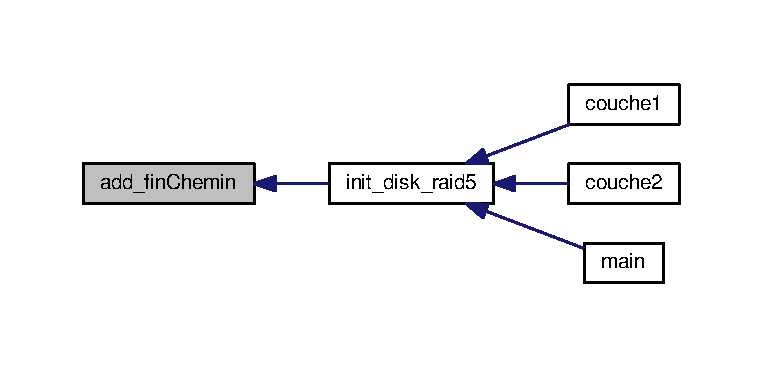
\includegraphics[width=350pt]{couche1_8c_a4479ca3bf5ef9da255dc34dd3b954b04_icgraph}
\end{center}
\end{figure}
\mbox{\Hypertarget{couche1_8c_a1a6021fbd31ca2b308d61050416ab520}\label{couche1_8c_a1a6021fbd31ca2b308d61050416ab520}} 
\index{couche1.\+c@{couche1.\+c}!affichage\+Block\+Decimal@{affichage\+Block\+Decimal}}
\index{affichage\+Block\+Decimal@{affichage\+Block\+Decimal}!couche1.\+c@{couche1.\+c}}
\subsubsection{\texorpdfstring{affichage\+Block\+Decimal()}{affichageBlockDecimal()}}
{\footnotesize\ttfamily int affichage\+Block\+Decimal (\begin{DoxyParamCaption}\item[{\hyperlink{raid__defines_8h_ab22cb9a2c3c081d95bd06c65d6716686}{virtual\+\_\+disk\+\_\+t} $\ast$}]{R\+A\+I\+D5,  }\item[{int}]{id\+Disk,  }\item[{\hyperlink{raid__defines_8h_a91ad9478d81a7aaf2593e8d9c3d06a14}{uint}}]{pos,  }\item[{F\+I\+LE $\ast$}]{output }\end{DoxyParamCaption})}



Definition at line 291 of file couche1.\+c.

Here is the call graph for this function\+:
\nopagebreak
\begin{figure}[H]
\begin{center}
\leavevmode
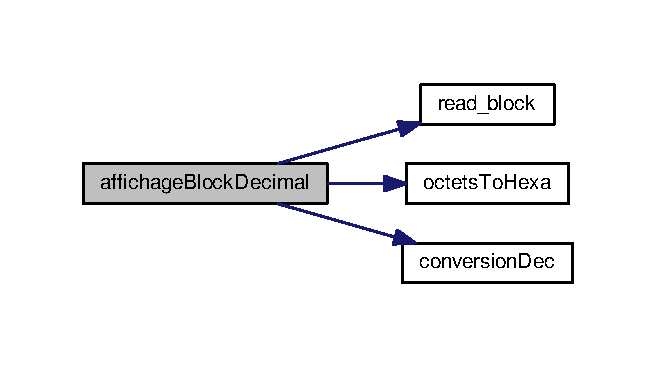
\includegraphics[width=315pt]{couche1_8c_a1a6021fbd31ca2b308d61050416ab520_cgraph}
\end{center}
\end{figure}
Here is the caller graph for this function\+:
\nopagebreak
\begin{figure}[H]
\begin{center}
\leavevmode
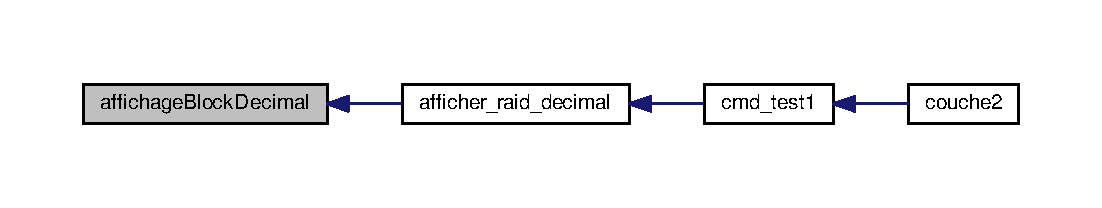
\includegraphics[width=350pt]{couche1_8c_a1a6021fbd31ca2b308d61050416ab520_icgraph}
\end{center}
\end{figure}
\mbox{\Hypertarget{couche1_8c_ae6cedff3423d9b8afe126d3f298576ee}\label{couche1_8c_ae6cedff3423d9b8afe126d3f298576ee}} 
\index{couche1.\+c@{couche1.\+c}!affichage\+Block\+Hexa@{affichage\+Block\+Hexa}}
\index{affichage\+Block\+Hexa@{affichage\+Block\+Hexa}!couche1.\+c@{couche1.\+c}}
\subsubsection{\texorpdfstring{affichage\+Block\+Hexa()}{affichageBlockHexa()}}
{\footnotesize\ttfamily int affichage\+Block\+Hexa (\begin{DoxyParamCaption}\item[{\hyperlink{raid__defines_8h_ab22cb9a2c3c081d95bd06c65d6716686}{virtual\+\_\+disk\+\_\+t} $\ast$}]{R\+A\+I\+D5,  }\item[{int}]{id\+Disk,  }\item[{\hyperlink{raid__defines_8h_a91ad9478d81a7aaf2593e8d9c3d06a14}{uint}}]{pos,  }\item[{F\+I\+LE $\ast$}]{output }\end{DoxyParamCaption})}



affiche un bloc de donnees en hexadecimal 


\begin{DoxyParams}{Parameters}
{\em } & virtual\+\_\+disk\+\_\+t \\
\hline
{\em } & integer (n° disk) \\
\hline
{\em } & integer (posit° de ce qu\textquotesingle{}on veut afficher) \\
\hline
\end{DoxyParams}
\begin{DoxyReturn}{Returns}
\+: void 
\end{DoxyReturn}


Definition at line 274 of file couche1.\+c.

Here is the call graph for this function\+:
\nopagebreak
\begin{figure}[H]
\begin{center}
\leavevmode
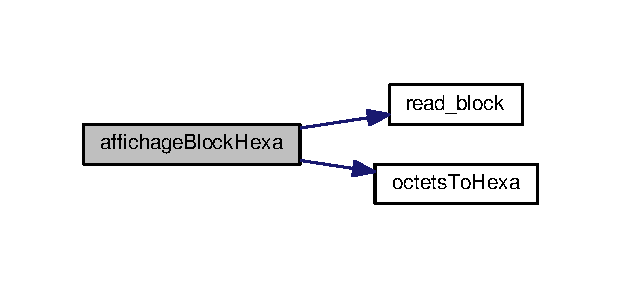
\includegraphics[width=298pt]{couche1_8c_ae6cedff3423d9b8afe126d3f298576ee_cgraph}
\end{center}
\end{figure}
Here is the caller graph for this function\+:
\nopagebreak
\begin{figure}[H]
\begin{center}
\leavevmode
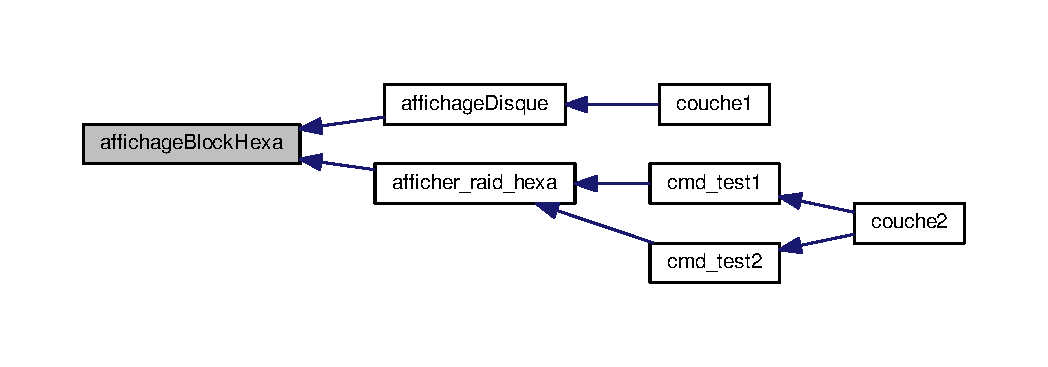
\includegraphics[width=350pt]{couche1_8c_ae6cedff3423d9b8afe126d3f298576ee_icgraph}
\end{center}
\end{figure}
\mbox{\Hypertarget{couche1_8c_a89f4e036d129f8952aa6711c9551ebc9}\label{couche1_8c_a89f4e036d129f8952aa6711c9551ebc9}} 
\index{couche1.\+c@{couche1.\+c}!affichage\+Disque@{affichage\+Disque}}
\index{affichage\+Disque@{affichage\+Disque}!couche1.\+c@{couche1.\+c}}
\subsubsection{\texorpdfstring{affichage\+Disque()}{affichageDisque()}}
{\footnotesize\ttfamily void affichage\+Disque (\begin{DoxyParamCaption}\item[{\hyperlink{raid__defines_8h_ab22cb9a2c3c081d95bd06c65d6716686}{virtual\+\_\+disk\+\_\+t} $\ast$}]{R\+A\+I\+D5,  }\item[{int}]{id\+Disk,  }\item[{F\+I\+LE $\ast$}]{output }\end{DoxyParamCaption})}



Definition at line 311 of file couche1.\+c.

Here is the call graph for this function\+:
\nopagebreak
\begin{figure}[H]
\begin{center}
\leavevmode
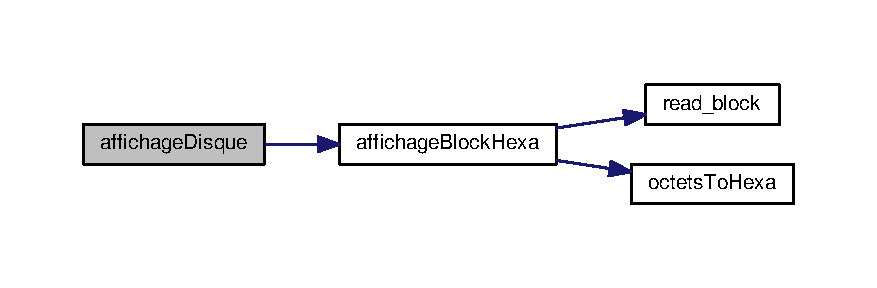
\includegraphics[width=350pt]{couche1_8c_a89f4e036d129f8952aa6711c9551ebc9_cgraph}
\end{center}
\end{figure}
Here is the caller graph for this function\+:
\nopagebreak
\begin{figure}[H]
\begin{center}
\leavevmode
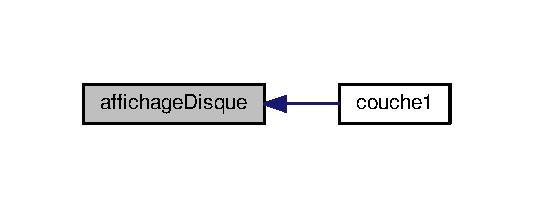
\includegraphics[width=256pt]{couche1_8c_a89f4e036d129f8952aa6711c9551ebc9_icgraph}
\end{center}
\end{figure}
\mbox{\Hypertarget{couche1_8c_a2035024bc72d159d51a6ef54a8dc978a}\label{couche1_8c_a2035024bc72d159d51a6ef54a8dc978a}} 
\index{couche1.\+c@{couche1.\+c}!block\+\_\+repair@{block\+\_\+repair}}
\index{block\+\_\+repair@{block\+\_\+repair}!couche1.\+c@{couche1.\+c}}
\subsubsection{\texorpdfstring{block\+\_\+repair()}{block\_repair()}}
{\footnotesize\ttfamily void block\+\_\+repair (\begin{DoxyParamCaption}\item[{\hyperlink{raid__defines_8h_ab22cb9a2c3c081d95bd06c65d6716686}{virtual\+\_\+disk\+\_\+t} $\ast$}]{R\+A\+I\+D5,  }\item[{\hyperlink{raid__defines_8h_a91ad9478d81a7aaf2593e8d9c3d06a14}{uint}}]{pos,  }\item[{int}]{id\+Disk }\end{DoxyParamCaption})}



Definition at line 163 of file couche1.\+c.

Here is the call graph for this function\+:
\nopagebreak
\begin{figure}[H]
\begin{center}
\leavevmode
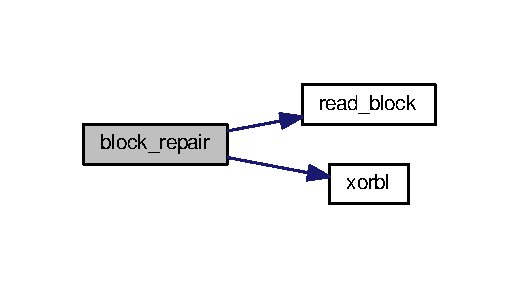
\includegraphics[width=249pt]{couche1_8c_a2035024bc72d159d51a6ef54a8dc978a_cgraph}
\end{center}
\end{figure}
\mbox{\Hypertarget{couche1_8c_a9cd7d6dccecc07ca1b67fd05c7928ee3}\label{couche1_8c_a9cd7d6dccecc07ca1b67fd05c7928ee3}} 
\index{couche1.\+c@{couche1.\+c}!compute\+\_\+nblock@{compute\+\_\+nblock}}
\index{compute\+\_\+nblock@{compute\+\_\+nblock}!couche1.\+c@{couche1.\+c}}
\subsubsection{\texorpdfstring{compute\+\_\+nblock()}{compute\_nblock()}}
{\footnotesize\ttfamily int compute\+\_\+nblock (\begin{DoxyParamCaption}\item[{int}]{n }\end{DoxyParamCaption})}



calcule le nombre de blocs pour coder \char`\"{}n\char`\"{} octets 


\begin{DoxyParams}{Parameters}
{\em integer} & \\
\hline
\end{DoxyParams}
\begin{DoxyReturn}{Returns}
integer 
\end{DoxyReturn}


Definition at line 93 of file couche1.\+c.

Here is the caller graph for this function\+:
\nopagebreak
\begin{figure}[H]
\begin{center}
\leavevmode
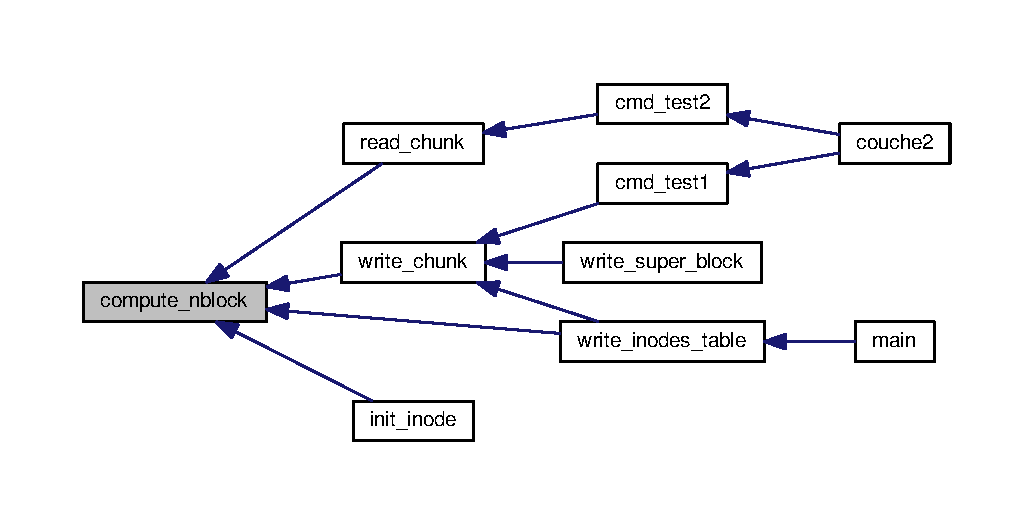
\includegraphics[width=350pt]{couche1_8c_a9cd7d6dccecc07ca1b67fd05c7928ee3_icgraph}
\end{center}
\end{figure}
\mbox{\Hypertarget{couche1_8c_a23fbb0c056aa4bfabd0cfd7b793591a3}\label{couche1_8c_a23fbb0c056aa4bfabd0cfd7b793591a3}} 
\index{couche1.\+c@{couche1.\+c}!conversion\+Dec@{conversion\+Dec}}
\index{conversion\+Dec@{conversion\+Dec}!couche1.\+c@{couche1.\+c}}
\subsubsection{\texorpdfstring{conversion\+Dec()}{conversionDec()}}
{\footnotesize\ttfamily int conversion\+Dec (\begin{DoxyParamCaption}\item[{int}]{nb4bits }\end{DoxyParamCaption})}



Definition at line 226 of file couche1.\+c.

Here is the caller graph for this function\+:
\nopagebreak
\begin{figure}[H]
\begin{center}
\leavevmode
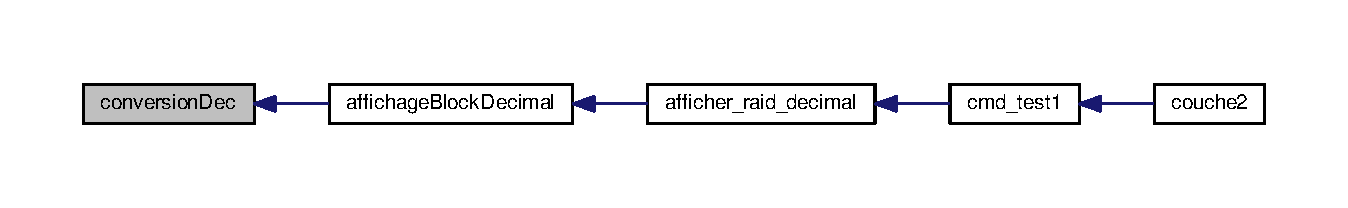
\includegraphics[width=350pt]{couche1_8c_a23fbb0c056aa4bfabd0cfd7b793591a3_icgraph}
\end{center}
\end{figure}
\mbox{\Hypertarget{couche1_8c_a7951420cc967a37ca46209305481727b}\label{couche1_8c_a7951420cc967a37ca46209305481727b}} 
\index{couche1.\+c@{couche1.\+c}!conversion\+Hexa@{conversion\+Hexa}}
\index{conversion\+Hexa@{conversion\+Hexa}!couche1.\+c@{couche1.\+c}}
\subsubsection{\texorpdfstring{conversion\+Hexa()}{conversionHexa()}}
{\footnotesize\ttfamily char conversion\+Hexa (\begin{DoxyParamCaption}\item[{char}]{nb4bits }\end{DoxyParamCaption})}



transforme un nombre en son chiffre en hexa 


\begin{DoxyParams}{Parameters}
{\em } & nb4bits, la valeur de 4 bits en entier \\
\hline
\end{DoxyParams}
\begin{DoxyReturn}{Returns}
\+: le chiffre en hexadecimal 
\end{DoxyReturn}


Definition at line 207 of file couche1.\+c.

Here is the caller graph for this function\+:
\nopagebreak
\begin{figure}[H]
\begin{center}
\leavevmode
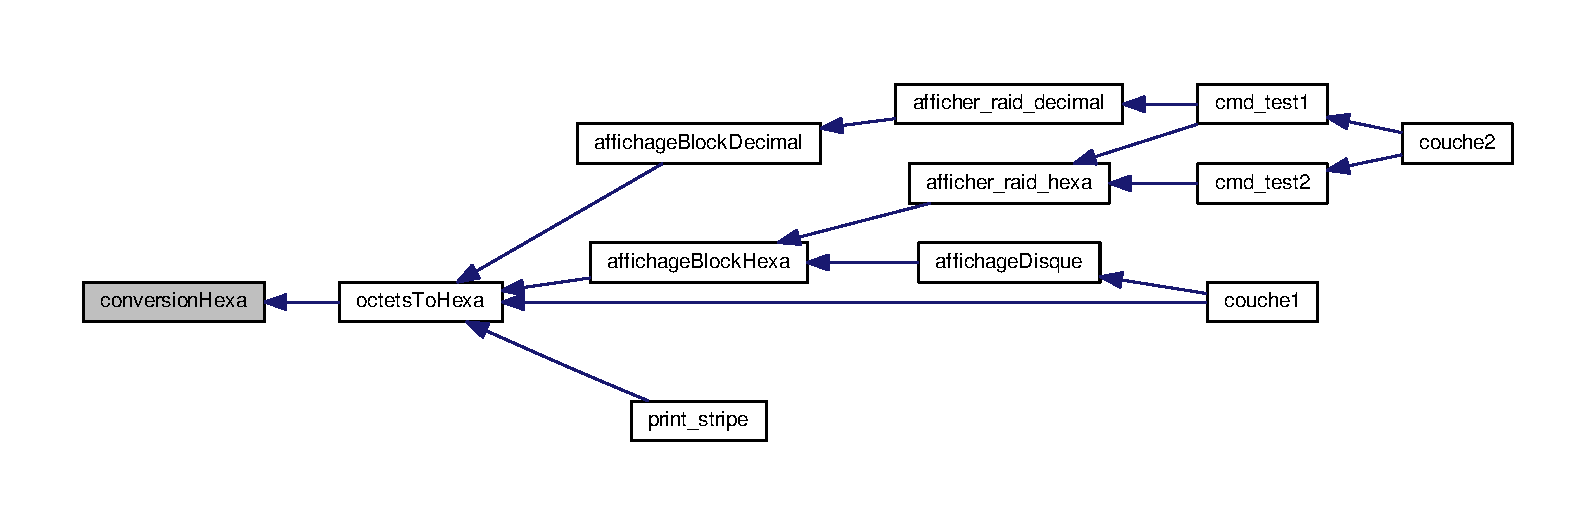
\includegraphics[width=350pt]{couche1_8c_a7951420cc967a37ca46209305481727b_icgraph}
\end{center}
\end{figure}
\mbox{\Hypertarget{couche1_8c_a778282843931610565cf6a8353a633bc}\label{couche1_8c_a778282843931610565cf6a8353a633bc}} 
\index{couche1.\+c@{couche1.\+c}!couche1@{couche1}}
\index{couche1@{couche1}!couche1.\+c@{couche1.\+c}}
\subsubsection{\texorpdfstring{couche1()}{couche1()}}
{\footnotesize\ttfamily int couche1 (\begin{DoxyParamCaption}\item[{void}]{ }\end{DoxyParamCaption})}



Definition at line 319 of file couche1.\+c.

Here is the call graph for this function\+:
\nopagebreak
\begin{figure}[H]
\begin{center}
\leavevmode
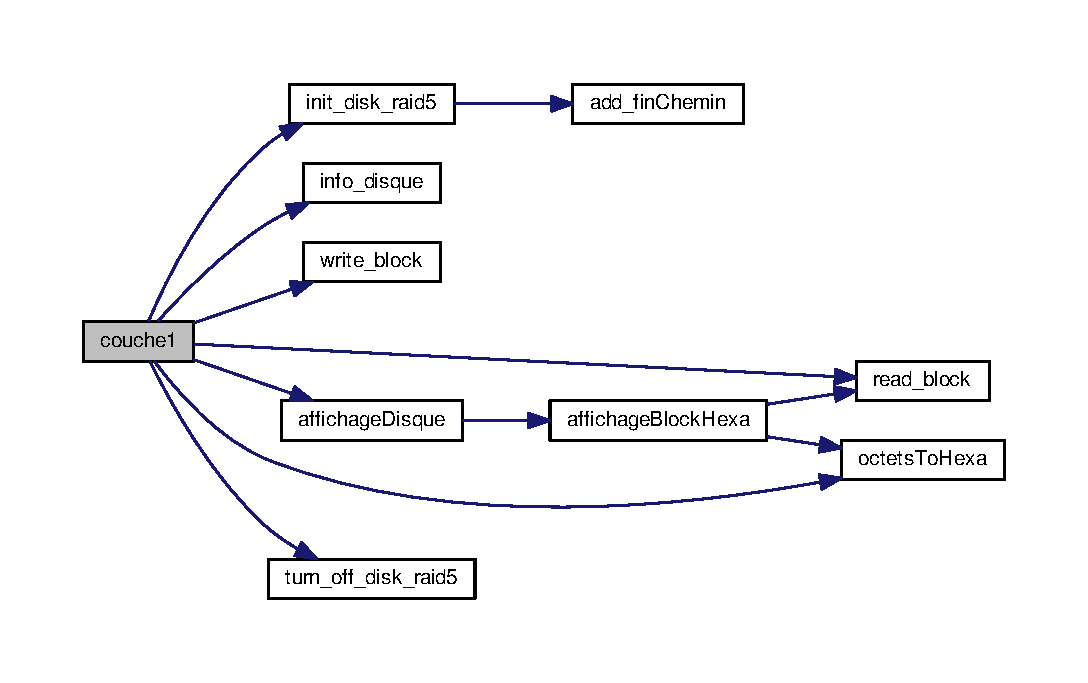
\includegraphics[width=350pt]{couche1_8c_a778282843931610565cf6a8353a633bc_cgraph}
\end{center}
\end{figure}
\mbox{\Hypertarget{couche1_8c_a988f68f7bebc679f512c8eadaa391f16}\label{couche1_8c_a988f68f7bebc679f512c8eadaa391f16}} 
\index{couche1.\+c@{couche1.\+c}!info\+\_\+disque@{info\+\_\+disque}}
\index{info\+\_\+disque@{info\+\_\+disque}!couche1.\+c@{couche1.\+c}}
\subsubsection{\texorpdfstring{info\+\_\+disque()}{info\_disque()}}
{\footnotesize\ttfamily void info\+\_\+disque (\begin{DoxyParamCaption}\item[{\hyperlink{raid__defines_8h_ab22cb9a2c3c081d95bd06c65d6716686}{virtual\+\_\+disk\+\_\+t} $\ast$}]{r5\+Disk }\end{DoxyParamCaption})}



Affiche des infos sur les disques ouverts. 


\begin{DoxyParams}{Parameters}
{\em } & virtual\+\_\+disk\+\_\+t \\
\hline
\end{DoxyParams}
\begin{DoxyReturn}{Returns}
\+: void 
\end{DoxyReturn}


Definition at line 79 of file couche1.\+c.

Here is the caller graph for this function\+:
\nopagebreak
\begin{figure}[H]
\begin{center}
\leavevmode
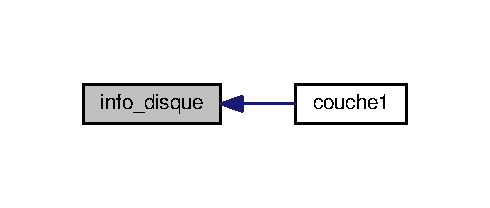
\includegraphics[width=235pt]{couche1_8c_a988f68f7bebc679f512c8eadaa391f16_icgraph}
\end{center}
\end{figure}
\mbox{\Hypertarget{couche1_8c_a745e214ead4cfa64503c1be97c30d25a}\label{couche1_8c_a745e214ead4cfa64503c1be97c30d25a}} 
\index{couche1.\+c@{couche1.\+c}!init\+\_\+disk\+\_\+raid5@{init\+\_\+disk\+\_\+raid5}}
\index{init\+\_\+disk\+\_\+raid5@{init\+\_\+disk\+\_\+raid5}!couche1.\+c@{couche1.\+c}}
\subsubsection{\texorpdfstring{init\+\_\+disk\+\_\+raid5()}{init\_disk\_raid5()}}
{\footnotesize\ttfamily void init\+\_\+disk\+\_\+raid5 (\begin{DoxyParamCaption}\item[{const char $\ast$}]{repertoire,  }\item[{\hyperlink{raid__defines_8h_ab22cb9a2c3c081d95bd06c65d6716686}{virtual\+\_\+disk\+\_\+t} $\ast$}]{r5\+Disk }\end{DoxyParamCaption})}



Initialise la variable globale r5\+Disk. 


\begin{DoxyParams}{Parameters}
{\em } & chaine de char (repertoire cible) \\
\hline
{\em } & virtual\+\_\+disk\+\_\+t \\
\hline
\end{DoxyParams}
\begin{DoxyReturn}{Returns}
void 
\end{DoxyReturn}


Definition at line 44 of file couche1.\+c.

Here is the call graph for this function\+:
\nopagebreak
\begin{figure}[H]
\begin{center}
\leavevmode
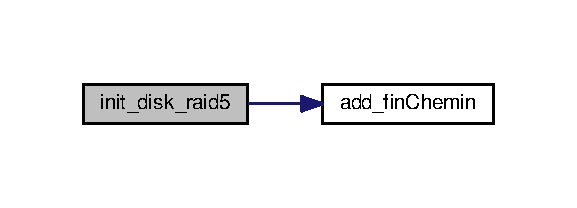
\includegraphics[width=277pt]{couche1_8c_a745e214ead4cfa64503c1be97c30d25a_cgraph}
\end{center}
\end{figure}
Here is the caller graph for this function\+:
\nopagebreak
\begin{figure}[H]
\begin{center}
\leavevmode
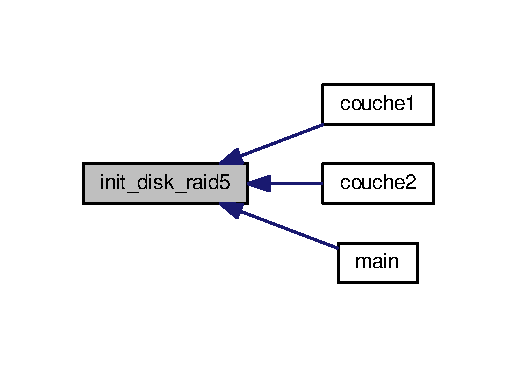
\includegraphics[width=248pt]{couche1_8c_a745e214ead4cfa64503c1be97c30d25a_icgraph}
\end{center}
\end{figure}
\mbox{\Hypertarget{couche1_8c_a1fc20a5afdea4eec626e52a499ff46cd}\label{couche1_8c_a1fc20a5afdea4eec626e52a499ff46cd}} 
\index{couche1.\+c@{couche1.\+c}!octets\+To\+Hexa@{octets\+To\+Hexa}}
\index{octets\+To\+Hexa@{octets\+To\+Hexa}!couche1.\+c@{couche1.\+c}}
\subsubsection{\texorpdfstring{octets\+To\+Hexa()}{octetsToHexa()}}
{\footnotesize\ttfamily void octets\+To\+Hexa (\begin{DoxyParamCaption}\item[{\hyperlink{raid__defines_8h_a9497df9c1d65b018066a9760da7be4e6}{block\+\_\+t}}]{mon\+Bloc,  }\item[{char $\ast$}]{nb\+Hexa }\end{DoxyParamCaption})}



prend un tableau de 4 octets (char) et le transforme en Hexadecimal assert(mon\+Bloc\mbox{[}i\mbox{]}$<$256); 


\begin{DoxyParams}{Parameters}
{\em } & block\+\_\+t (Contient le tableau de bits) \\
\hline
{\em } & char$\ast$ (Caractere dans lequel on met l\textquotesingle{}hexa) \\
\hline
\end{DoxyParams}
\begin{DoxyReturn}{Returns}
\+: void 
\end{DoxyReturn}


Definition at line 192 of file couche1.\+c.

Here is the caller graph for this function\+:
\nopagebreak
\begin{figure}[H]
\begin{center}
\leavevmode
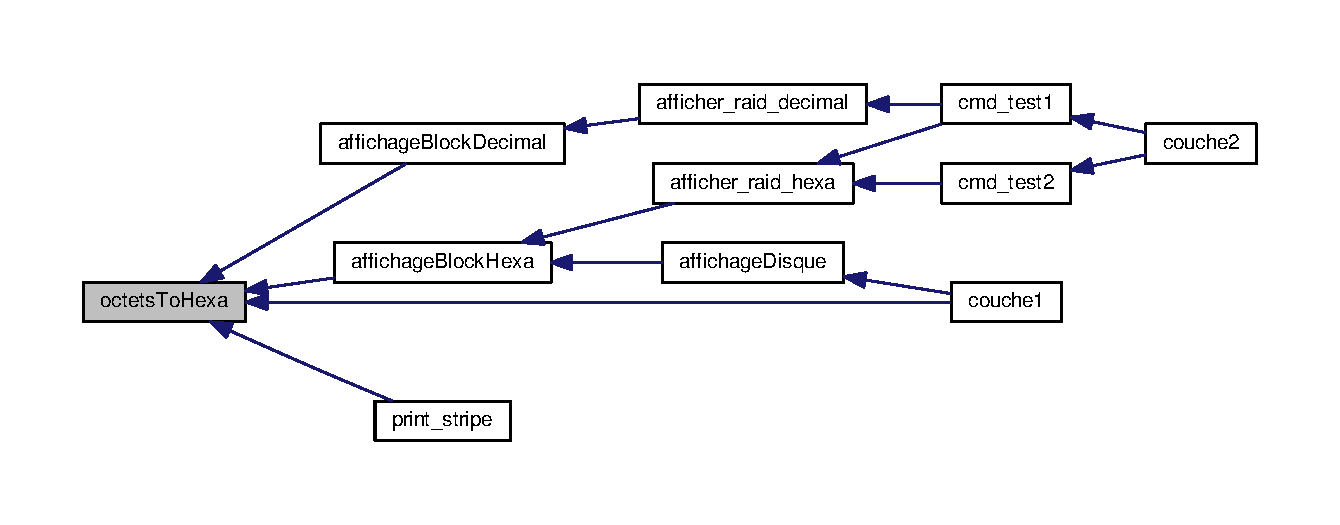
\includegraphics[width=350pt]{couche1_8c_a1fc20a5afdea4eec626e52a499ff46cd_icgraph}
\end{center}
\end{figure}
\mbox{\Hypertarget{couche1_8c_a4ba30a1143e543d465725eb0f151c6a2}\label{couche1_8c_a4ba30a1143e543d465725eb0f151c6a2}} 
\index{couche1.\+c@{couche1.\+c}!read\+\_\+block@{read\+\_\+block}}
\index{read\+\_\+block@{read\+\_\+block}!couche1.\+c@{couche1.\+c}}
\subsubsection{\texorpdfstring{read\+\_\+block()}{read\_block()}}
{\footnotesize\ttfamily int read\+\_\+block (\begin{DoxyParamCaption}\item[{\hyperlink{raid__defines_8h_ab22cb9a2c3c081d95bd06c65d6716686}{virtual\+\_\+disk\+\_\+t} $\ast$}]{R\+A\+I\+D5,  }\item[{\hyperlink{raid__defines_8h_a9497df9c1d65b018066a9760da7be4e6}{block\+\_\+t} $\ast$}]{recup,  }\item[{\hyperlink{raid__defines_8h_a91ad9478d81a7aaf2593e8d9c3d06a14}{uint}}]{pos,  }\item[{int}]{id\+Disk }\end{DoxyParamCaption})}



Lit un bloc à la position pos sur le disque. 


\begin{DoxyParams}{Parameters}
{\em virtual\+\_\+disk\+\_\+t} & \\
\hline
{\em block\+\_\+t} & (à lire) \\
\hline
{\em uint} & (position à laquelle on lit) \\
\hline
{\em integer} & (n° disk) \\
\hline
\end{DoxyParams}
\begin{DoxyReturn}{Returns}
integer 
\end{DoxyReturn}


Definition at line 130 of file couche1.\+c.

Here is the caller graph for this function\+:
\nopagebreak
\begin{figure}[H]
\begin{center}
\leavevmode
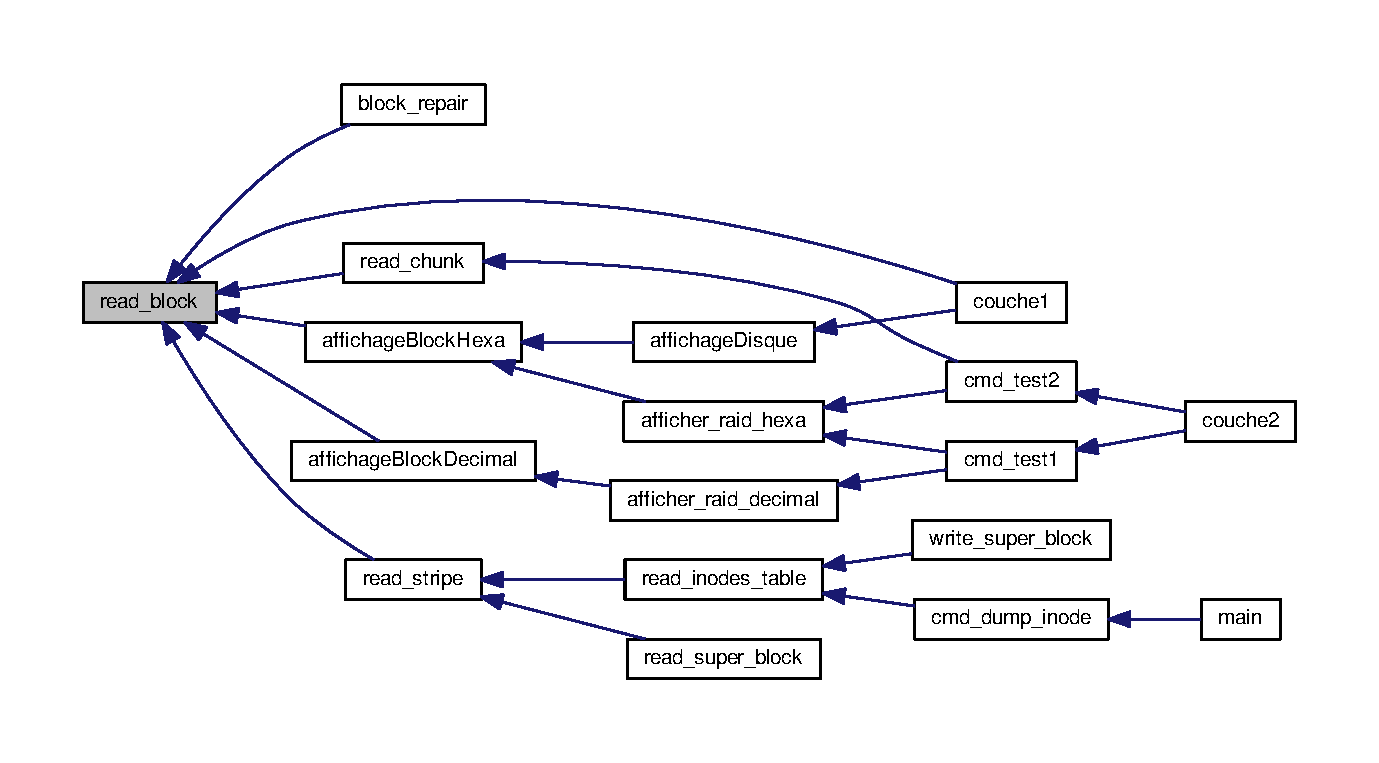
\includegraphics[width=350pt]{couche1_8c_a4ba30a1143e543d465725eb0f151c6a2_icgraph}
\end{center}
\end{figure}
\mbox{\Hypertarget{couche1_8c_a0f31c284e3b9461448ae2c5393a4c53f}\label{couche1_8c_a0f31c284e3b9461448ae2c5393a4c53f}} 
\index{couche1.\+c@{couche1.\+c}!turn\+\_\+off\+\_\+disk\+\_\+raid5@{turn\+\_\+off\+\_\+disk\+\_\+raid5}}
\index{turn\+\_\+off\+\_\+disk\+\_\+raid5@{turn\+\_\+off\+\_\+disk\+\_\+raid5}!couche1.\+c@{couche1.\+c}}
\subsubsection{\texorpdfstring{turn\+\_\+off\+\_\+disk\+\_\+raid5()}{turn\_off\_disk\_raid5()}}
{\footnotesize\ttfamily void turn\+\_\+off\+\_\+disk\+\_\+raid5 (\begin{DoxyParamCaption}\item[{\hyperlink{raid__defines_8h_ab22cb9a2c3c081d95bd06c65d6716686}{virtual\+\_\+disk\+\_\+t} $\ast$}]{r5\+Disk }\end{DoxyParamCaption})}



Ferme les fichiers ouverts et sauvegarde le super block? 


\begin{DoxyParams}{Parameters}
{\em } & chaine de char (repertoire cible) \\
\hline
{\em } & virtual\+\_\+disk\+\_\+t \\
\hline
\end{DoxyParams}
\begin{DoxyReturn}{Returns}
void 
\end{DoxyReturn}


Definition at line 66 of file couche1.\+c.

Here is the caller graph for this function\+:
\nopagebreak
\begin{figure}[H]
\begin{center}
\leavevmode
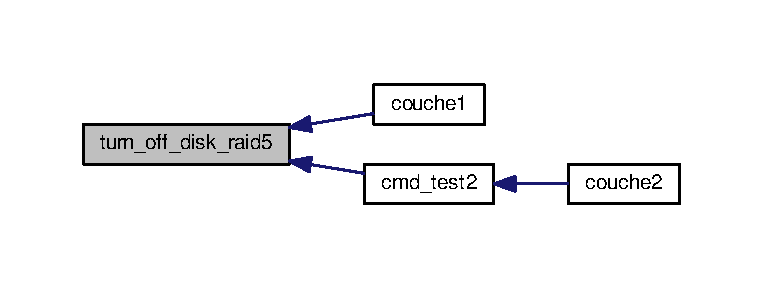
\includegraphics[width=350pt]{couche1_8c_a0f31c284e3b9461448ae2c5393a4c53f_icgraph}
\end{center}
\end{figure}
\mbox{\Hypertarget{couche1_8c_adb4607cf11ffed5c89fc0f4682bf6079}\label{couche1_8c_adb4607cf11ffed5c89fc0f4682bf6079}} 
\index{couche1.\+c@{couche1.\+c}!write\+\_\+block@{write\+\_\+block}}
\index{write\+\_\+block@{write\+\_\+block}!couche1.\+c@{couche1.\+c}}
\subsubsection{\texorpdfstring{write\+\_\+block()}{write\_block()}}
{\footnotesize\ttfamily void write\+\_\+block (\begin{DoxyParamCaption}\item[{\hyperlink{raid__defines_8h_ab22cb9a2c3c081d95bd06c65d6716686}{virtual\+\_\+disk\+\_\+t} $\ast$}]{R\+A\+I\+D5,  }\item[{\hyperlink{raid__defines_8h_a9497df9c1d65b018066a9760da7be4e6}{block\+\_\+t} $\ast$}]{entrant,  }\item[{\hyperlink{raid__defines_8h_a91ad9478d81a7aaf2593e8d9c3d06a14}{uint}}]{pos,  }\item[{int}]{id\+Disk }\end{DoxyParamCaption})}



Ecrit un bloc à la position pos sur le disque. 


\begin{DoxyParams}{Parameters}
{\em virtual\+\_\+disk\+\_\+t} & \\
\hline
{\em block\+\_\+t} & (à ecrire) \\
\hline
{\em uint} & (position à laquelle on ecrit) \\
\hline
{\em integer} & (n° disk) \\
\hline
\end{DoxyParams}
\begin{DoxyReturn}{Returns}
void 
\end{DoxyReturn}


Definition at line 112 of file couche1.\+c.

Here is the caller graph for this function\+:
\nopagebreak
\begin{figure}[H]
\begin{center}
\leavevmode
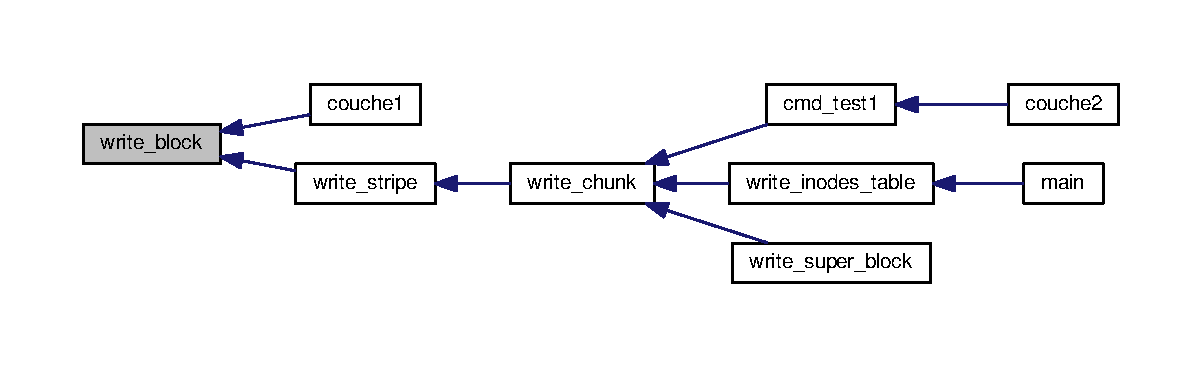
\includegraphics[width=350pt]{couche1_8c_adb4607cf11ffed5c89fc0f4682bf6079_icgraph}
\end{center}
\end{figure}
\mbox{\Hypertarget{couche1_8c_a69d295ba0ccd1a14fbc7ef4dd2c3a5c9}\label{couche1_8c_a69d295ba0ccd1a14fbc7ef4dd2c3a5c9}} 
\index{couche1.\+c@{couche1.\+c}!xorbl@{xorbl}}
\index{xorbl@{xorbl}!couche1.\+c@{couche1.\+c}}
\subsubsection{\texorpdfstring{xorbl()}{xorbl()}}
{\footnotesize\ttfamily void xorbl (\begin{DoxyParamCaption}\item[{\hyperlink{raid__defines_8h_a9497df9c1d65b018066a9760da7be4e6}{block\+\_\+t} $\ast$}]{xa,  }\item[{\hyperlink{raid__defines_8h_a9497df9c1d65b018066a9760da7be4e6}{block\+\_\+t} $\ast$}]{xb,  }\item[{\hyperlink{raid__defines_8h_a9497df9c1d65b018066a9760da7be4e6}{block\+\_\+t} $\ast$}]{destination }\end{DoxyParamCaption})}



Definition at line 141 of file couche1.\+c.

Here is the caller graph for this function\+:
\nopagebreak
\begin{figure}[H]
\begin{center}
\leavevmode
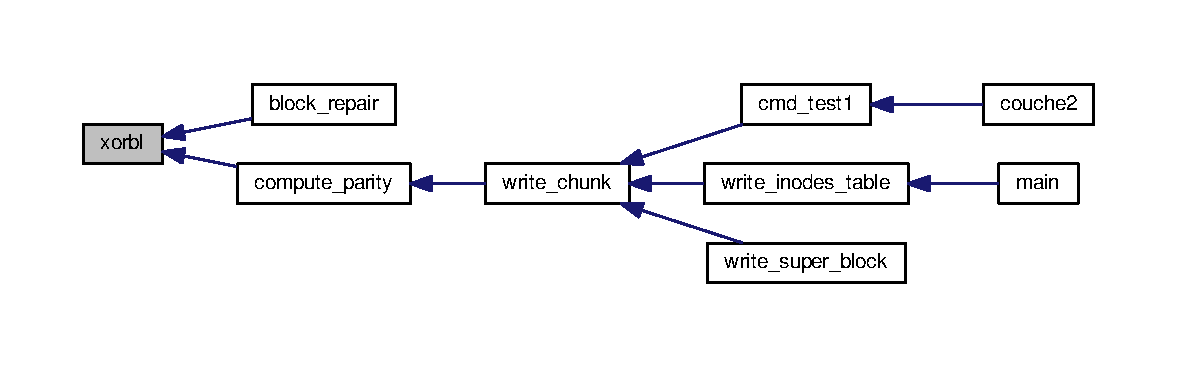
\includegraphics[width=350pt]{couche1_8c_a69d295ba0ccd1a14fbc7ef4dd2c3a5c9_icgraph}
\end{center}
\end{figure}

\hypertarget{couche1_8h}{}\section{couche1.\+h File Reference}
\label{couche1_8h}\index{couche1.\+h@{couche1.\+h}}
{\ttfamily \#include \char`\"{}raid\+\_\+defines.\+h\char`\"{}}\newline
Include dependency graph for couche1.\+h\+:
\nopagebreak
\begin{figure}[H]
\begin{center}
\leavevmode
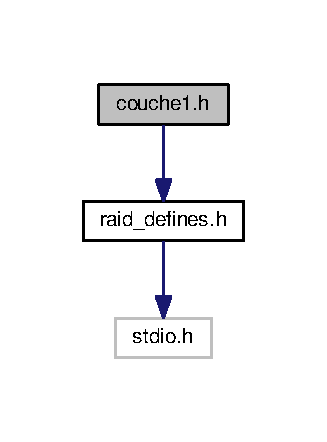
\includegraphics[width=157pt]{couche1_8h__incl}
\end{center}
\end{figure}
This graph shows which files directly or indirectly include this file\+:
\nopagebreak
\begin{figure}[H]
\begin{center}
\leavevmode
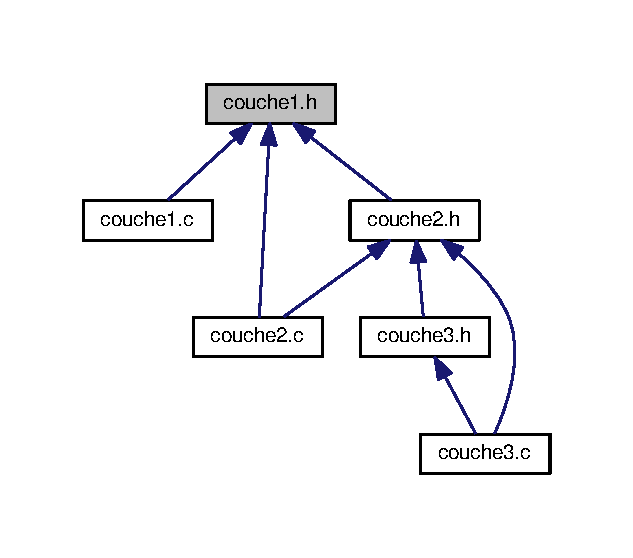
\includegraphics[width=304pt]{couche1_8h__dep__incl}
\end{center}
\end{figure}
\subsection*{Functions}
\begin{DoxyCompactItemize}
\item 
void \hyperlink{couche1_8h_a4479ca3bf5ef9da255dc34dd3b954b04}{add\+\_\+fin\+Chemin} (const char $\ast$repertoire, char $\ast$nom\+Disque, size\+\_\+t length\+Rep)
\begin{DoxyCompactList}\small\item\em Copie la chaine \char`\"{}repertoire\char`\"{} dans nom\+Disque en y ajoutant \char`\"{}/d0\textbackslash{}0\char`\"{}. \end{DoxyCompactList}\item 
void \hyperlink{couche1_8h_a745e214ead4cfa64503c1be97c30d25a}{init\+\_\+disk\+\_\+raid5} (const char $\ast$repertoire, \hyperlink{raid__defines_8h_ab22cb9a2c3c081d95bd06c65d6716686}{virtual\+\_\+disk\+\_\+t} $\ast$\hyperlink{trash_8c_aa32bee7663041ae13a36afeae68a3f14}{r5\+Disk})
\begin{DoxyCompactList}\small\item\em Initialise la variable globale r5\+Disk. \end{DoxyCompactList}\item 
void \hyperlink{couche1_8h_a0f31c284e3b9461448ae2c5393a4c53f}{turn\+\_\+off\+\_\+disk\+\_\+raid5} (\hyperlink{raid__defines_8h_ab22cb9a2c3c081d95bd06c65d6716686}{virtual\+\_\+disk\+\_\+t} $\ast$\hyperlink{trash_8c_aa32bee7663041ae13a36afeae68a3f14}{r5\+Disk})
\begin{DoxyCompactList}\small\item\em Ferme les fichiers ouverts et sauvegarde le super block? \end{DoxyCompactList}\item 
void \hyperlink{couche1_8h_a988f68f7bebc679f512c8eadaa391f16}{info\+\_\+disque} (\hyperlink{raid__defines_8h_ab22cb9a2c3c081d95bd06c65d6716686}{virtual\+\_\+disk\+\_\+t} $\ast$\hyperlink{trash_8c_aa32bee7663041ae13a36afeae68a3f14}{r5\+Disk})
\begin{DoxyCompactList}\small\item\em Affiche des infos sur les disques ouverts. \end{DoxyCompactList}\item 
int \hyperlink{couche1_8h_a9cd7d6dccecc07ca1b67fd05c7928ee3}{compute\+\_\+nblock} (int n)
\begin{DoxyCompactList}\small\item\em calcule le nombre de blocs pour coder \char`\"{}n\char`\"{} octets \end{DoxyCompactList}\item 
void \hyperlink{couche1_8h_adb4607cf11ffed5c89fc0f4682bf6079}{write\+\_\+block} (\hyperlink{raid__defines_8h_ab22cb9a2c3c081d95bd06c65d6716686}{virtual\+\_\+disk\+\_\+t} $\ast$R\+A\+I\+D5, \hyperlink{raid__defines_8h_a9497df9c1d65b018066a9760da7be4e6}{block\+\_\+t} $\ast$entrant, \hyperlink{raid__defines_8h_a91ad9478d81a7aaf2593e8d9c3d06a14}{uint} pos, int id\+Disk)
\begin{DoxyCompactList}\small\item\em Ecrit un bloc à la position pos sur le disque. \end{DoxyCompactList}\item 
int \hyperlink{couche1_8h_a4ba30a1143e543d465725eb0f151c6a2}{read\+\_\+block} (\hyperlink{raid__defines_8h_ab22cb9a2c3c081d95bd06c65d6716686}{virtual\+\_\+disk\+\_\+t} $\ast$R\+A\+I\+D5, \hyperlink{raid__defines_8h_a9497df9c1d65b018066a9760da7be4e6}{block\+\_\+t} $\ast$recup, \hyperlink{raid__defines_8h_a91ad9478d81a7aaf2593e8d9c3d06a14}{uint} pos, int id\+Disk)
\begin{DoxyCompactList}\small\item\em Lit un bloc à la position pos sur le disque. \end{DoxyCompactList}\item 
void \hyperlink{couche1_8h_a2035024bc72d159d51a6ef54a8dc978a}{block\+\_\+repair} (\hyperlink{raid__defines_8h_ab22cb9a2c3c081d95bd06c65d6716686}{virtual\+\_\+disk\+\_\+t} $\ast$R\+A\+I\+D5, \hyperlink{raid__defines_8h_a91ad9478d81a7aaf2593e8d9c3d06a14}{uint} pos, int id\+Disk)
\item 
void \hyperlink{couche1_8h_a1fc20a5afdea4eec626e52a499ff46cd}{octets\+To\+Hexa} (\hyperlink{raid__defines_8h_a9497df9c1d65b018066a9760da7be4e6}{block\+\_\+t} mon\+Bloc, char $\ast$nb\+Hexa)
\begin{DoxyCompactList}\small\item\em prend un tableau de 4 octets (char) et le transforme en Hexadecimal assert(mon\+Bloc\mbox{[}i\mbox{]}$<$256); \end{DoxyCompactList}\item 
int \hyperlink{couche1_8h_ae6cedff3423d9b8afe126d3f298576ee}{affichage\+Block\+Hexa} (\hyperlink{raid__defines_8h_ab22cb9a2c3c081d95bd06c65d6716686}{virtual\+\_\+disk\+\_\+t} $\ast$R\+A\+I\+D5, int id\+Disk, \hyperlink{raid__defines_8h_a91ad9478d81a7aaf2593e8d9c3d06a14}{uint} pos, F\+I\+LE $\ast$output)
\begin{DoxyCompactList}\small\item\em affiche un bloc de donnees en hexadecimal \end{DoxyCompactList}\item 
int \hyperlink{couche1_8h_a1a6021fbd31ca2b308d61050416ab520}{affichage\+Block\+Decimal} (\hyperlink{raid__defines_8h_ab22cb9a2c3c081d95bd06c65d6716686}{virtual\+\_\+disk\+\_\+t} $\ast$R\+A\+I\+D5, int id\+Disk, \hyperlink{raid__defines_8h_a91ad9478d81a7aaf2593e8d9c3d06a14}{uint} pos, F\+I\+LE $\ast$output)
\item 
char \hyperlink{couche1_8h_a7951420cc967a37ca46209305481727b}{conversion\+Hexa} (char nb4bits)
\begin{DoxyCompactList}\small\item\em transforme un nombre en son chiffre en hexa \end{DoxyCompactList}\item 
void \hyperlink{couche1_8h_a69d295ba0ccd1a14fbc7ef4dd2c3a5c9}{xorbl} (\hyperlink{raid__defines_8h_a9497df9c1d65b018066a9760da7be4e6}{block\+\_\+t} $\ast$xa, \hyperlink{raid__defines_8h_a9497df9c1d65b018066a9760da7be4e6}{block\+\_\+t} $\ast$xb, \hyperlink{raid__defines_8h_a9497df9c1d65b018066a9760da7be4e6}{block\+\_\+t} $\ast$destination)
\item 
int \hyperlink{couche1_8h_a778282843931610565cf6a8353a633bc}{couche1} (void)
\item 
void \hyperlink{couche1_8h_a89f4e036d129f8952aa6711c9551ebc9}{affichage\+Disque} (\hyperlink{raid__defines_8h_ab22cb9a2c3c081d95bd06c65d6716686}{virtual\+\_\+disk\+\_\+t} $\ast$R\+A\+I\+D5, int id\+Disk, F\+I\+LE $\ast$output)
\item 
int \hyperlink{couche1_8h_a23fbb0c056aa4bfabd0cfd7b793591a3}{conversion\+Dec} (int nb4bits)
\end{DoxyCompactItemize}


\subsection{Function Documentation}
\mbox{\Hypertarget{couche1_8h_a4479ca3bf5ef9da255dc34dd3b954b04}\label{couche1_8h_a4479ca3bf5ef9da255dc34dd3b954b04}} 
\index{couche1.\+h@{couche1.\+h}!add\+\_\+fin\+Chemin@{add\+\_\+fin\+Chemin}}
\index{add\+\_\+fin\+Chemin@{add\+\_\+fin\+Chemin}!couche1.\+h@{couche1.\+h}}
\subsubsection{\texorpdfstring{add\+\_\+fin\+Chemin()}{add\_finChemin()}}
{\footnotesize\ttfamily void add\+\_\+fin\+Chemin (\begin{DoxyParamCaption}\item[{const char $\ast$}]{repertoire,  }\item[{char $\ast$}]{nom\+Disque,  }\item[{size\+\_\+t}]{length\+Rep }\end{DoxyParamCaption})}



Copie la chaine \char`\"{}repertoire\char`\"{} dans nom\+Disque en y ajoutant \char`\"{}/d0\textbackslash{}0\char`\"{}. 


\begin{DoxyParams}{Parameters}
{\em } & chaine de char (repertoire) \\
\hline
{\em } & chaine de char (disk) \\
\hline
{\em } & size\+\_\+t \\
\hline
\end{DoxyParams}
\begin{DoxyReturn}{Returns}
void 
\end{DoxyReturn}


Definition at line 29 of file couche1.\+c.

Here is the caller graph for this function\+:
\nopagebreak
\begin{figure}[H]
\begin{center}
\leavevmode
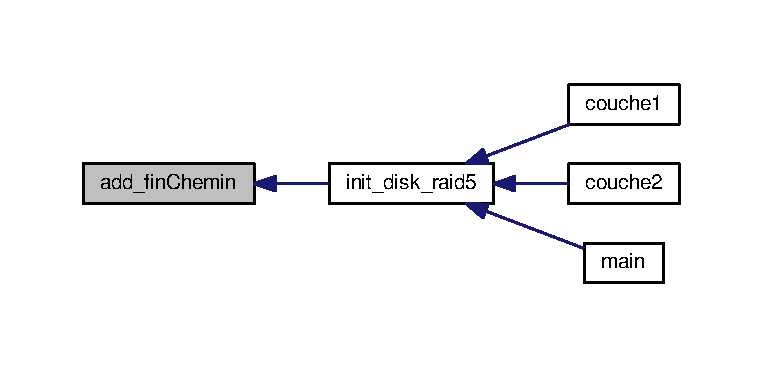
\includegraphics[width=350pt]{couche1_8h_a4479ca3bf5ef9da255dc34dd3b954b04_icgraph}
\end{center}
\end{figure}
\mbox{\Hypertarget{couche1_8h_a1a6021fbd31ca2b308d61050416ab520}\label{couche1_8h_a1a6021fbd31ca2b308d61050416ab520}} 
\index{couche1.\+h@{couche1.\+h}!affichage\+Block\+Decimal@{affichage\+Block\+Decimal}}
\index{affichage\+Block\+Decimal@{affichage\+Block\+Decimal}!couche1.\+h@{couche1.\+h}}
\subsubsection{\texorpdfstring{affichage\+Block\+Decimal()}{affichageBlockDecimal()}}
{\footnotesize\ttfamily int affichage\+Block\+Decimal (\begin{DoxyParamCaption}\item[{\hyperlink{raid__defines_8h_ab22cb9a2c3c081d95bd06c65d6716686}{virtual\+\_\+disk\+\_\+t} $\ast$}]{R\+A\+I\+D5,  }\item[{int}]{id\+Disk,  }\item[{\hyperlink{raid__defines_8h_a91ad9478d81a7aaf2593e8d9c3d06a14}{uint}}]{pos,  }\item[{F\+I\+LE $\ast$}]{output }\end{DoxyParamCaption})}



Definition at line 291 of file couche1.\+c.

Here is the call graph for this function\+:
\nopagebreak
\begin{figure}[H]
\begin{center}
\leavevmode
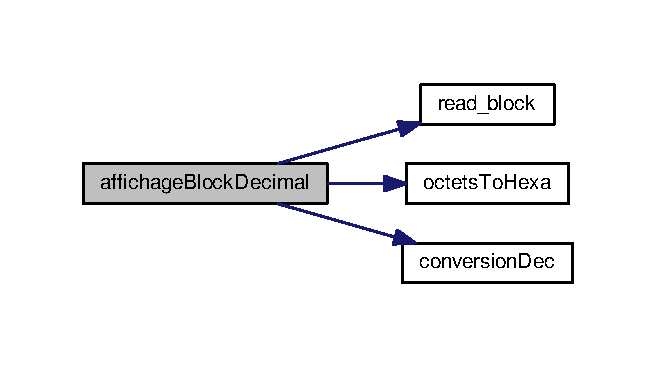
\includegraphics[width=315pt]{couche1_8h_a1a6021fbd31ca2b308d61050416ab520_cgraph}
\end{center}
\end{figure}
Here is the caller graph for this function\+:
\nopagebreak
\begin{figure}[H]
\begin{center}
\leavevmode
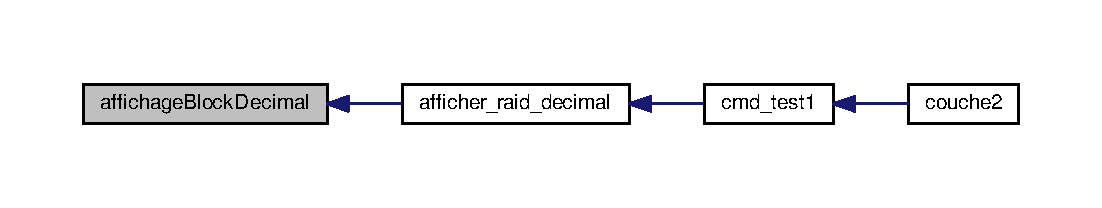
\includegraphics[width=350pt]{couche1_8h_a1a6021fbd31ca2b308d61050416ab520_icgraph}
\end{center}
\end{figure}
\mbox{\Hypertarget{couche1_8h_ae6cedff3423d9b8afe126d3f298576ee}\label{couche1_8h_ae6cedff3423d9b8afe126d3f298576ee}} 
\index{couche1.\+h@{couche1.\+h}!affichage\+Block\+Hexa@{affichage\+Block\+Hexa}}
\index{affichage\+Block\+Hexa@{affichage\+Block\+Hexa}!couche1.\+h@{couche1.\+h}}
\subsubsection{\texorpdfstring{affichage\+Block\+Hexa()}{affichageBlockHexa()}}
{\footnotesize\ttfamily int affichage\+Block\+Hexa (\begin{DoxyParamCaption}\item[{\hyperlink{raid__defines_8h_ab22cb9a2c3c081d95bd06c65d6716686}{virtual\+\_\+disk\+\_\+t} $\ast$}]{R\+A\+I\+D5,  }\item[{int}]{id\+Disk,  }\item[{\hyperlink{raid__defines_8h_a91ad9478d81a7aaf2593e8d9c3d06a14}{uint}}]{pos,  }\item[{F\+I\+LE $\ast$}]{output }\end{DoxyParamCaption})}



affiche un bloc de donnees en hexadecimal 


\begin{DoxyParams}{Parameters}
{\em } & virtual\+\_\+disk\+\_\+t \\
\hline
{\em } & integer (n° disk) \\
\hline
{\em } & integer (posit° de ce qu\textquotesingle{}on veut afficher) \\
\hline
\end{DoxyParams}
\begin{DoxyReturn}{Returns}
\+: void 
\end{DoxyReturn}


Definition at line 274 of file couche1.\+c.

Here is the call graph for this function\+:
\nopagebreak
\begin{figure}[H]
\begin{center}
\leavevmode
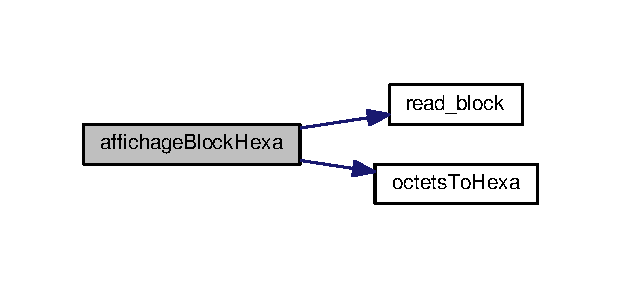
\includegraphics[width=298pt]{couche1_8h_ae6cedff3423d9b8afe126d3f298576ee_cgraph}
\end{center}
\end{figure}
Here is the caller graph for this function\+:
\nopagebreak
\begin{figure}[H]
\begin{center}
\leavevmode
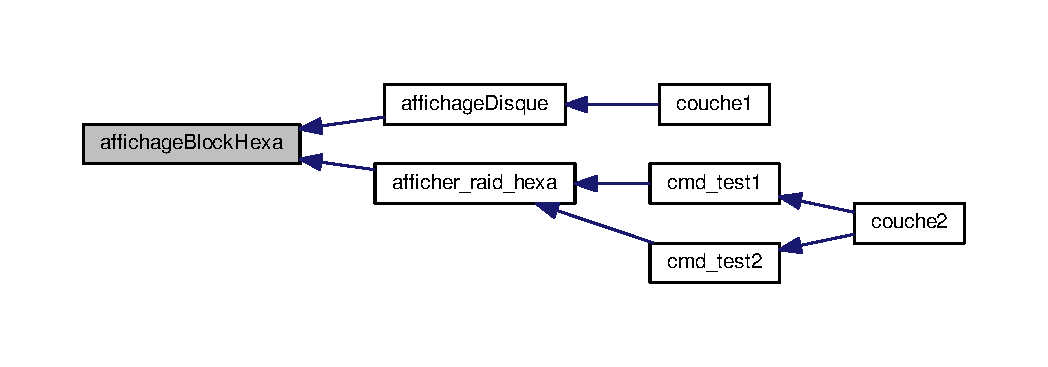
\includegraphics[width=350pt]{couche1_8h_ae6cedff3423d9b8afe126d3f298576ee_icgraph}
\end{center}
\end{figure}
\mbox{\Hypertarget{couche1_8h_a89f4e036d129f8952aa6711c9551ebc9}\label{couche1_8h_a89f4e036d129f8952aa6711c9551ebc9}} 
\index{couche1.\+h@{couche1.\+h}!affichage\+Disque@{affichage\+Disque}}
\index{affichage\+Disque@{affichage\+Disque}!couche1.\+h@{couche1.\+h}}
\subsubsection{\texorpdfstring{affichage\+Disque()}{affichageDisque()}}
{\footnotesize\ttfamily void affichage\+Disque (\begin{DoxyParamCaption}\item[{\hyperlink{raid__defines_8h_ab22cb9a2c3c081d95bd06c65d6716686}{virtual\+\_\+disk\+\_\+t} $\ast$}]{R\+A\+I\+D5,  }\item[{int}]{id\+Disk,  }\item[{F\+I\+LE $\ast$}]{output }\end{DoxyParamCaption})}



Definition at line 311 of file couche1.\+c.

Here is the call graph for this function\+:
\nopagebreak
\begin{figure}[H]
\begin{center}
\leavevmode
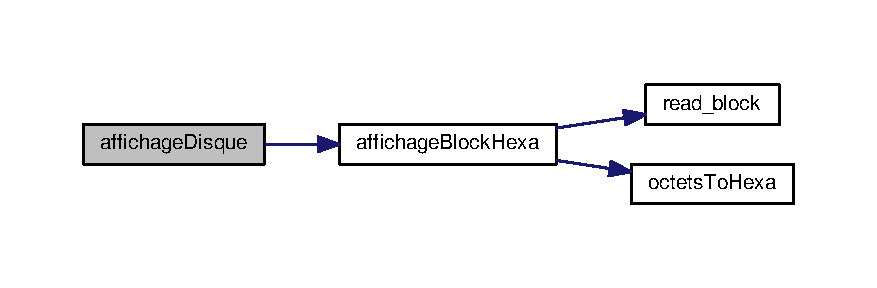
\includegraphics[width=350pt]{couche1_8h_a89f4e036d129f8952aa6711c9551ebc9_cgraph}
\end{center}
\end{figure}
Here is the caller graph for this function\+:
\nopagebreak
\begin{figure}[H]
\begin{center}
\leavevmode
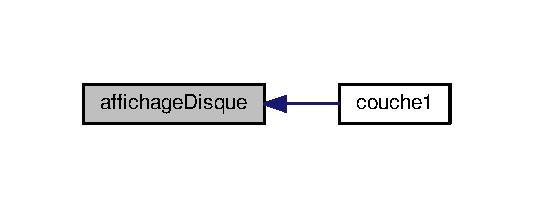
\includegraphics[width=256pt]{couche1_8h_a89f4e036d129f8952aa6711c9551ebc9_icgraph}
\end{center}
\end{figure}
\mbox{\Hypertarget{couche1_8h_a2035024bc72d159d51a6ef54a8dc978a}\label{couche1_8h_a2035024bc72d159d51a6ef54a8dc978a}} 
\index{couche1.\+h@{couche1.\+h}!block\+\_\+repair@{block\+\_\+repair}}
\index{block\+\_\+repair@{block\+\_\+repair}!couche1.\+h@{couche1.\+h}}
\subsubsection{\texorpdfstring{block\+\_\+repair()}{block\_repair()}}
{\footnotesize\ttfamily void block\+\_\+repair (\begin{DoxyParamCaption}\item[{\hyperlink{raid__defines_8h_ab22cb9a2c3c081d95bd06c65d6716686}{virtual\+\_\+disk\+\_\+t} $\ast$}]{R\+A\+I\+D5,  }\item[{\hyperlink{raid__defines_8h_a91ad9478d81a7aaf2593e8d9c3d06a14}{uint}}]{pos,  }\item[{int}]{id\+Disk }\end{DoxyParamCaption})}



Definition at line 163 of file couche1.\+c.

Here is the call graph for this function\+:
\nopagebreak
\begin{figure}[H]
\begin{center}
\leavevmode
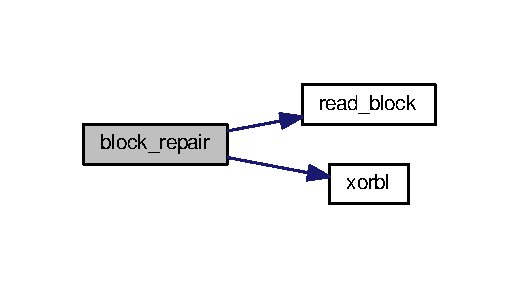
\includegraphics[width=249pt]{couche1_8h_a2035024bc72d159d51a6ef54a8dc978a_cgraph}
\end{center}
\end{figure}
\mbox{\Hypertarget{couche1_8h_a9cd7d6dccecc07ca1b67fd05c7928ee3}\label{couche1_8h_a9cd7d6dccecc07ca1b67fd05c7928ee3}} 
\index{couche1.\+h@{couche1.\+h}!compute\+\_\+nblock@{compute\+\_\+nblock}}
\index{compute\+\_\+nblock@{compute\+\_\+nblock}!couche1.\+h@{couche1.\+h}}
\subsubsection{\texorpdfstring{compute\+\_\+nblock()}{compute\_nblock()}}
{\footnotesize\ttfamily int compute\+\_\+nblock (\begin{DoxyParamCaption}\item[{int}]{n }\end{DoxyParamCaption})}



calcule le nombre de blocs pour coder \char`\"{}n\char`\"{} octets 


\begin{DoxyParams}{Parameters}
{\em integer} & \\
\hline
\end{DoxyParams}
\begin{DoxyReturn}{Returns}
integer 
\end{DoxyReturn}


Definition at line 93 of file couche1.\+c.

Here is the caller graph for this function\+:
\nopagebreak
\begin{figure}[H]
\begin{center}
\leavevmode
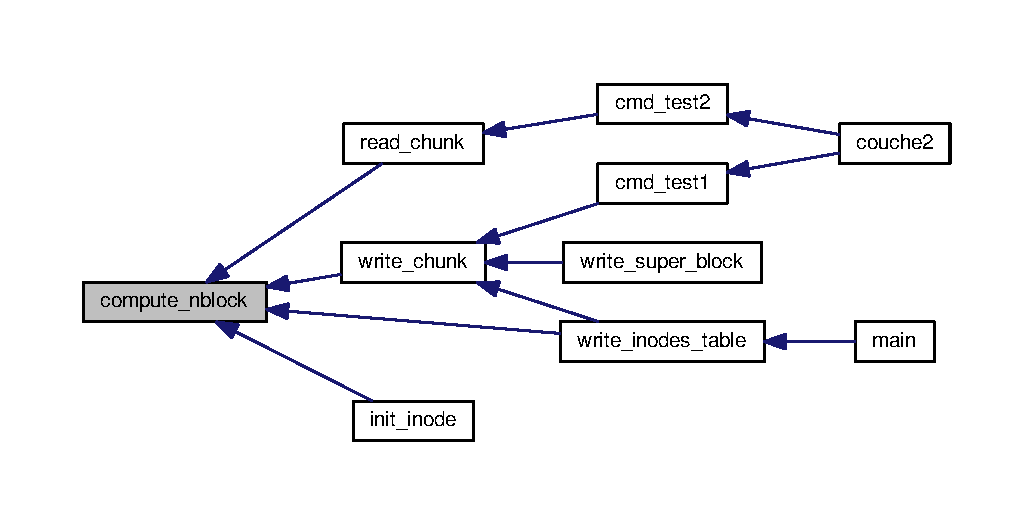
\includegraphics[width=350pt]{couche1_8h_a9cd7d6dccecc07ca1b67fd05c7928ee3_icgraph}
\end{center}
\end{figure}
\mbox{\Hypertarget{couche1_8h_a23fbb0c056aa4bfabd0cfd7b793591a3}\label{couche1_8h_a23fbb0c056aa4bfabd0cfd7b793591a3}} 
\index{couche1.\+h@{couche1.\+h}!conversion\+Dec@{conversion\+Dec}}
\index{conversion\+Dec@{conversion\+Dec}!couche1.\+h@{couche1.\+h}}
\subsubsection{\texorpdfstring{conversion\+Dec()}{conversionDec()}}
{\footnotesize\ttfamily int conversion\+Dec (\begin{DoxyParamCaption}\item[{int}]{nb4bits }\end{DoxyParamCaption})}



Definition at line 226 of file couche1.\+c.

Here is the caller graph for this function\+:
\nopagebreak
\begin{figure}[H]
\begin{center}
\leavevmode
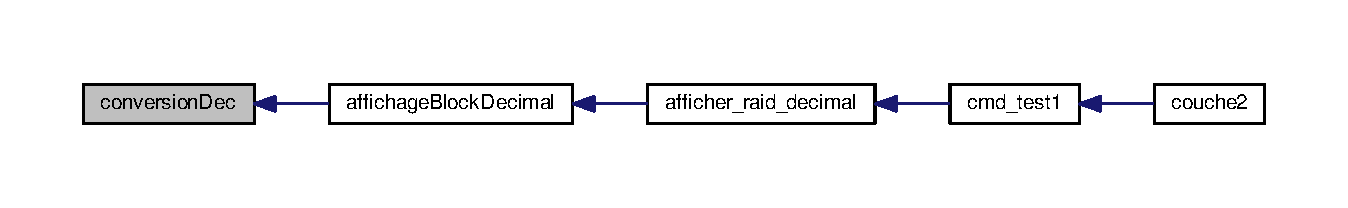
\includegraphics[width=350pt]{couche1_8h_a23fbb0c056aa4bfabd0cfd7b793591a3_icgraph}
\end{center}
\end{figure}
\mbox{\Hypertarget{couche1_8h_a7951420cc967a37ca46209305481727b}\label{couche1_8h_a7951420cc967a37ca46209305481727b}} 
\index{couche1.\+h@{couche1.\+h}!conversion\+Hexa@{conversion\+Hexa}}
\index{conversion\+Hexa@{conversion\+Hexa}!couche1.\+h@{couche1.\+h}}
\subsubsection{\texorpdfstring{conversion\+Hexa()}{conversionHexa()}}
{\footnotesize\ttfamily char conversion\+Hexa (\begin{DoxyParamCaption}\item[{char}]{nb4bits }\end{DoxyParamCaption})}



transforme un nombre en son chiffre en hexa 


\begin{DoxyParams}{Parameters}
{\em } & nb4bits, la valeur de 4 bits en entier \\
\hline
\end{DoxyParams}
\begin{DoxyReturn}{Returns}
\+: le chiffre en hexadecimal 
\end{DoxyReturn}


Definition at line 207 of file couche1.\+c.

Here is the caller graph for this function\+:
\nopagebreak
\begin{figure}[H]
\begin{center}
\leavevmode
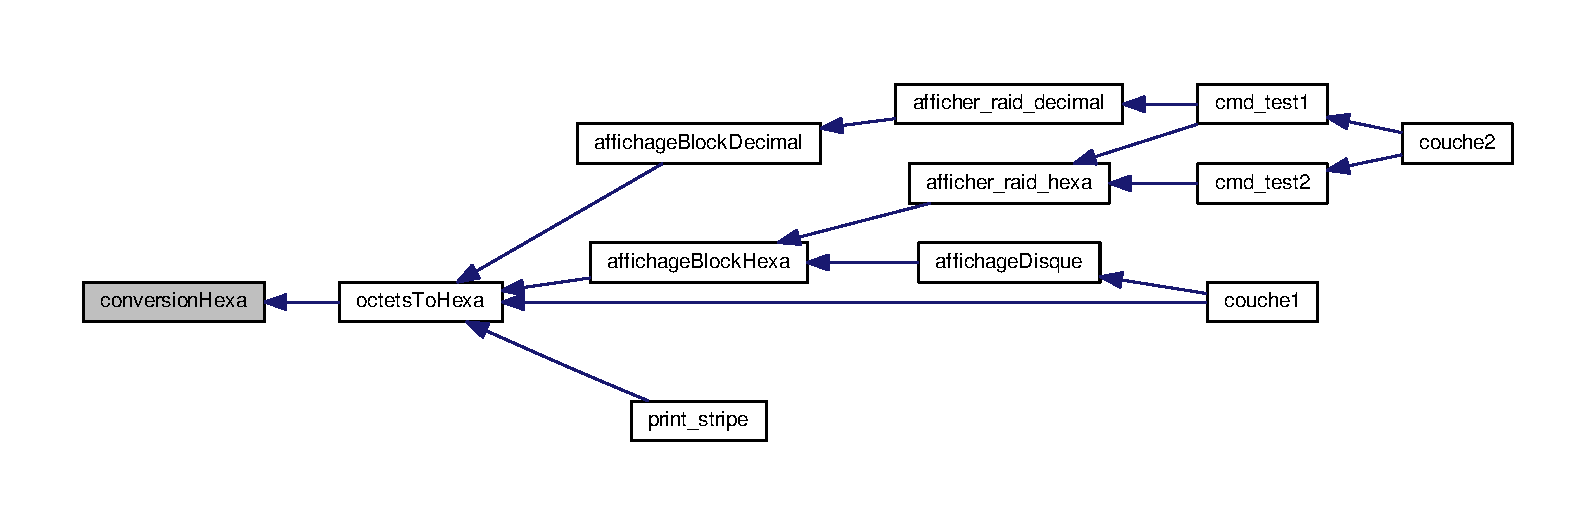
\includegraphics[width=350pt]{couche1_8h_a7951420cc967a37ca46209305481727b_icgraph}
\end{center}
\end{figure}
\mbox{\Hypertarget{couche1_8h_a778282843931610565cf6a8353a633bc}\label{couche1_8h_a778282843931610565cf6a8353a633bc}} 
\index{couche1.\+h@{couche1.\+h}!couche1@{couche1}}
\index{couche1@{couche1}!couche1.\+h@{couche1.\+h}}
\subsubsection{\texorpdfstring{couche1()}{couche1()}}
{\footnotesize\ttfamily int couche1 (\begin{DoxyParamCaption}\item[{void}]{ }\end{DoxyParamCaption})}



Definition at line 319 of file couche1.\+c.

Here is the call graph for this function\+:
\nopagebreak
\begin{figure}[H]
\begin{center}
\leavevmode
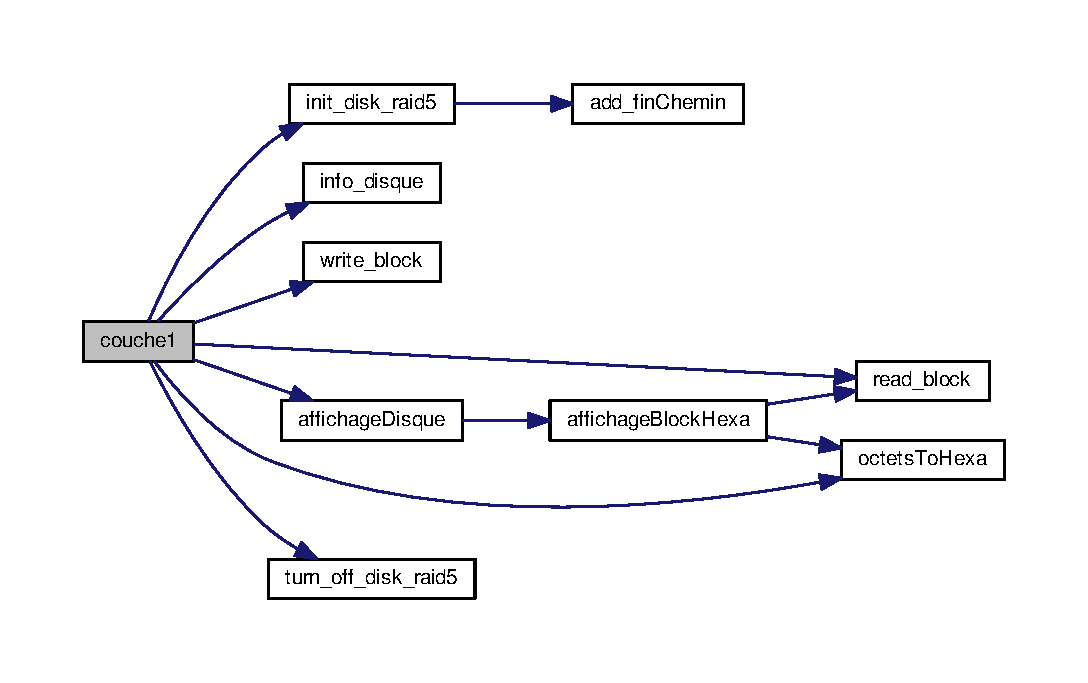
\includegraphics[width=350pt]{couche1_8h_a778282843931610565cf6a8353a633bc_cgraph}
\end{center}
\end{figure}
\mbox{\Hypertarget{couche1_8h_a988f68f7bebc679f512c8eadaa391f16}\label{couche1_8h_a988f68f7bebc679f512c8eadaa391f16}} 
\index{couche1.\+h@{couche1.\+h}!info\+\_\+disque@{info\+\_\+disque}}
\index{info\+\_\+disque@{info\+\_\+disque}!couche1.\+h@{couche1.\+h}}
\subsubsection{\texorpdfstring{info\+\_\+disque()}{info\_disque()}}
{\footnotesize\ttfamily void info\+\_\+disque (\begin{DoxyParamCaption}\item[{\hyperlink{raid__defines_8h_ab22cb9a2c3c081d95bd06c65d6716686}{virtual\+\_\+disk\+\_\+t} $\ast$}]{r5\+Disk }\end{DoxyParamCaption})}



Affiche des infos sur les disques ouverts. 


\begin{DoxyParams}{Parameters}
{\em } & virtual\+\_\+disk\+\_\+t \\
\hline
\end{DoxyParams}
\begin{DoxyReturn}{Returns}
\+: void 
\end{DoxyReturn}


Definition at line 79 of file couche1.\+c.

Here is the caller graph for this function\+:
\nopagebreak
\begin{figure}[H]
\begin{center}
\leavevmode
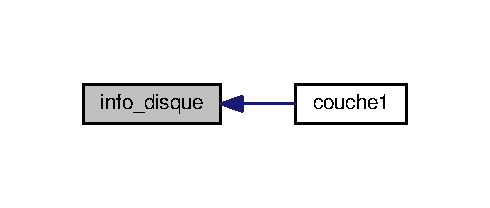
\includegraphics[width=235pt]{couche1_8h_a988f68f7bebc679f512c8eadaa391f16_icgraph}
\end{center}
\end{figure}
\mbox{\Hypertarget{couche1_8h_a745e214ead4cfa64503c1be97c30d25a}\label{couche1_8h_a745e214ead4cfa64503c1be97c30d25a}} 
\index{couche1.\+h@{couche1.\+h}!init\+\_\+disk\+\_\+raid5@{init\+\_\+disk\+\_\+raid5}}
\index{init\+\_\+disk\+\_\+raid5@{init\+\_\+disk\+\_\+raid5}!couche1.\+h@{couche1.\+h}}
\subsubsection{\texorpdfstring{init\+\_\+disk\+\_\+raid5()}{init\_disk\_raid5()}}
{\footnotesize\ttfamily void init\+\_\+disk\+\_\+raid5 (\begin{DoxyParamCaption}\item[{const char $\ast$}]{repertoire,  }\item[{\hyperlink{raid__defines_8h_ab22cb9a2c3c081d95bd06c65d6716686}{virtual\+\_\+disk\+\_\+t} $\ast$}]{r5\+Disk }\end{DoxyParamCaption})}



Initialise la variable globale r5\+Disk. 


\begin{DoxyParams}{Parameters}
{\em } & chaine de char (repertoire cible) \\
\hline
{\em } & virtual\+\_\+disk\+\_\+t \\
\hline
\end{DoxyParams}
\begin{DoxyReturn}{Returns}
void 
\end{DoxyReturn}


Definition at line 44 of file couche1.\+c.

Here is the call graph for this function\+:
\nopagebreak
\begin{figure}[H]
\begin{center}
\leavevmode
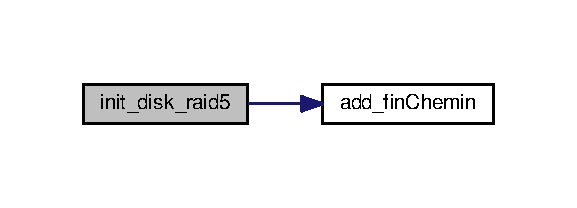
\includegraphics[width=277pt]{couche1_8h_a745e214ead4cfa64503c1be97c30d25a_cgraph}
\end{center}
\end{figure}
Here is the caller graph for this function\+:
\nopagebreak
\begin{figure}[H]
\begin{center}
\leavevmode
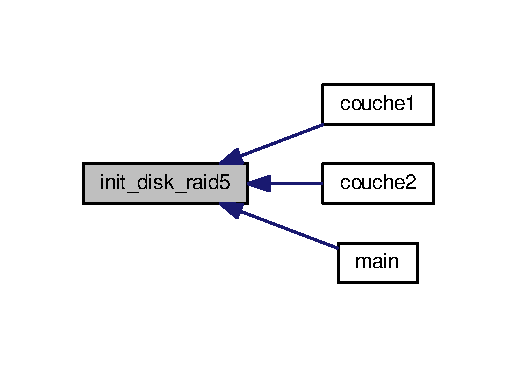
\includegraphics[width=248pt]{couche1_8h_a745e214ead4cfa64503c1be97c30d25a_icgraph}
\end{center}
\end{figure}
\mbox{\Hypertarget{couche1_8h_a1fc20a5afdea4eec626e52a499ff46cd}\label{couche1_8h_a1fc20a5afdea4eec626e52a499ff46cd}} 
\index{couche1.\+h@{couche1.\+h}!octets\+To\+Hexa@{octets\+To\+Hexa}}
\index{octets\+To\+Hexa@{octets\+To\+Hexa}!couche1.\+h@{couche1.\+h}}
\subsubsection{\texorpdfstring{octets\+To\+Hexa()}{octetsToHexa()}}
{\footnotesize\ttfamily void octets\+To\+Hexa (\begin{DoxyParamCaption}\item[{\hyperlink{raid__defines_8h_a9497df9c1d65b018066a9760da7be4e6}{block\+\_\+t}}]{mon\+Bloc,  }\item[{char $\ast$}]{nb\+Hexa }\end{DoxyParamCaption})}



prend un tableau de 4 octets (char) et le transforme en Hexadecimal assert(mon\+Bloc\mbox{[}i\mbox{]}$<$256); 


\begin{DoxyParams}{Parameters}
{\em } & block\+\_\+t (Contient le tableau de bits) \\
\hline
{\em } & char$\ast$ (Caractere dans lequel on met l\textquotesingle{}hexa) \\
\hline
\end{DoxyParams}
\begin{DoxyReturn}{Returns}
\+: void 
\end{DoxyReturn}


Definition at line 192 of file couche1.\+c.

Here is the call graph for this function\+:
\nopagebreak
\begin{figure}[H]
\begin{center}
\leavevmode
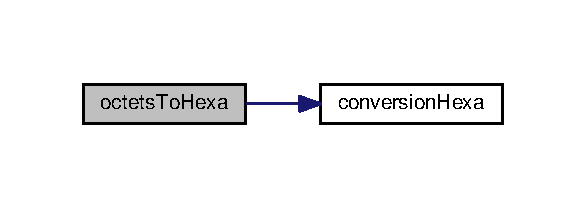
\includegraphics[width=281pt]{couche1_8h_a1fc20a5afdea4eec626e52a499ff46cd_cgraph}
\end{center}
\end{figure}
Here is the caller graph for this function\+:
\nopagebreak
\begin{figure}[H]
\begin{center}
\leavevmode
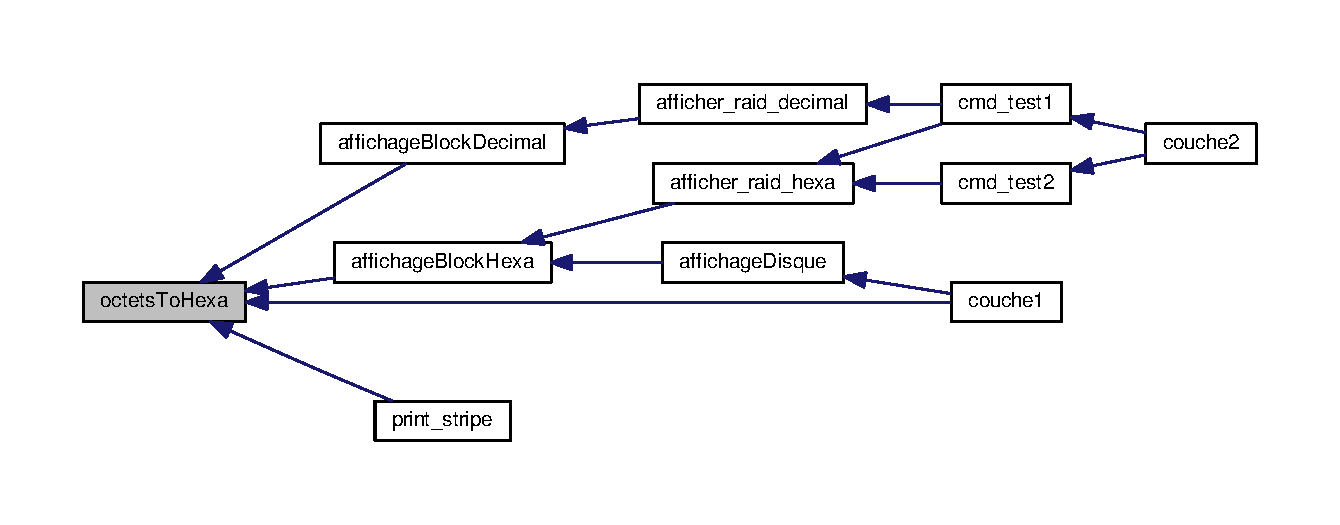
\includegraphics[width=350pt]{couche1_8h_a1fc20a5afdea4eec626e52a499ff46cd_icgraph}
\end{center}
\end{figure}
\mbox{\Hypertarget{couche1_8h_a4ba30a1143e543d465725eb0f151c6a2}\label{couche1_8h_a4ba30a1143e543d465725eb0f151c6a2}} 
\index{couche1.\+h@{couche1.\+h}!read\+\_\+block@{read\+\_\+block}}
\index{read\+\_\+block@{read\+\_\+block}!couche1.\+h@{couche1.\+h}}
\subsubsection{\texorpdfstring{read\+\_\+block()}{read\_block()}}
{\footnotesize\ttfamily int read\+\_\+block (\begin{DoxyParamCaption}\item[{\hyperlink{raid__defines_8h_ab22cb9a2c3c081d95bd06c65d6716686}{virtual\+\_\+disk\+\_\+t} $\ast$}]{R\+A\+I\+D5,  }\item[{\hyperlink{raid__defines_8h_a9497df9c1d65b018066a9760da7be4e6}{block\+\_\+t} $\ast$}]{recup,  }\item[{\hyperlink{raid__defines_8h_a91ad9478d81a7aaf2593e8d9c3d06a14}{uint}}]{pos,  }\item[{int}]{id\+Disk }\end{DoxyParamCaption})}



Lit un bloc à la position pos sur le disque. 


\begin{DoxyParams}{Parameters}
{\em virtual\+\_\+disk\+\_\+t} & \\
\hline
{\em block\+\_\+t} & (à lire) \\
\hline
{\em uint} & (position à laquelle on lit) \\
\hline
{\em integer} & (n° disk) \\
\hline
\end{DoxyParams}
\begin{DoxyReturn}{Returns}
integer 
\end{DoxyReturn}


Definition at line 130 of file couche1.\+c.

Here is the caller graph for this function\+:
\nopagebreak
\begin{figure}[H]
\begin{center}
\leavevmode
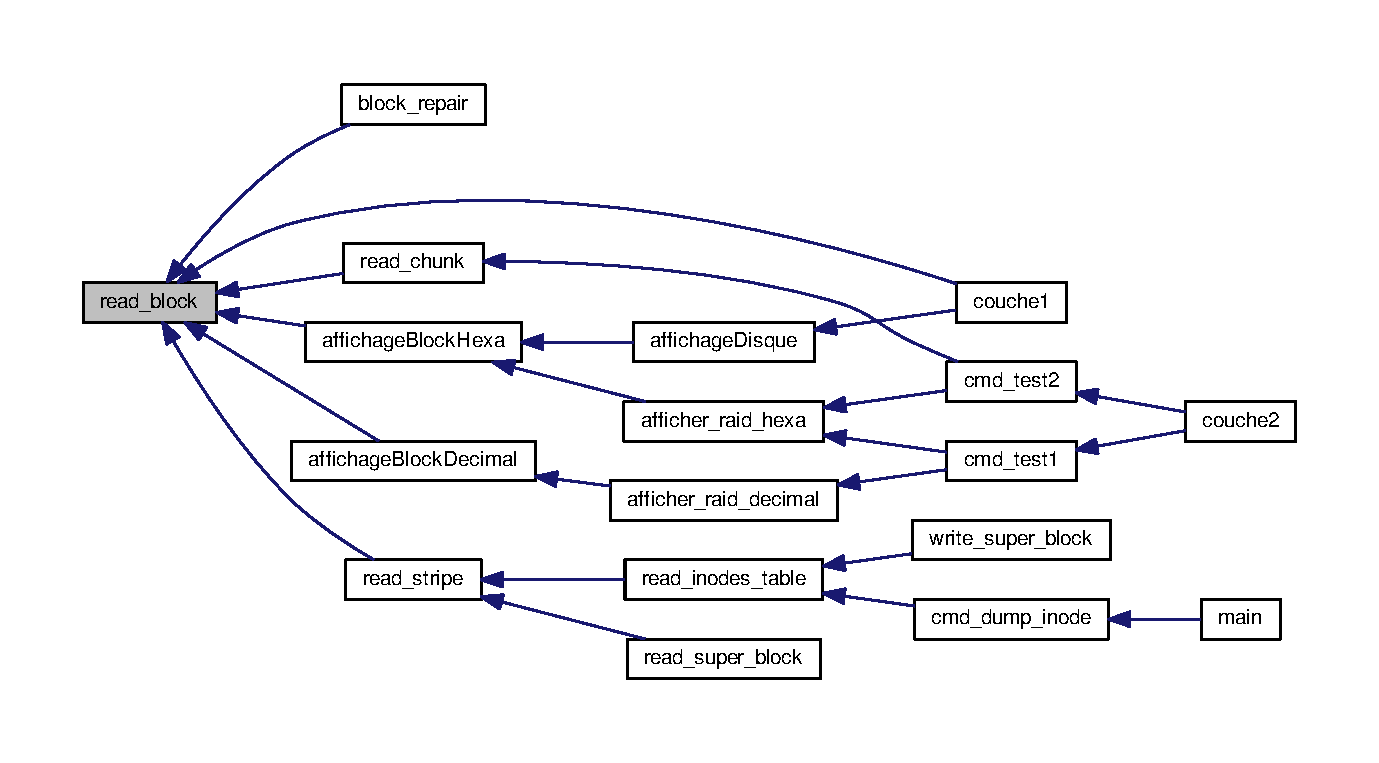
\includegraphics[width=350pt]{couche1_8h_a4ba30a1143e543d465725eb0f151c6a2_icgraph}
\end{center}
\end{figure}
\mbox{\Hypertarget{couche1_8h_a0f31c284e3b9461448ae2c5393a4c53f}\label{couche1_8h_a0f31c284e3b9461448ae2c5393a4c53f}} 
\index{couche1.\+h@{couche1.\+h}!turn\+\_\+off\+\_\+disk\+\_\+raid5@{turn\+\_\+off\+\_\+disk\+\_\+raid5}}
\index{turn\+\_\+off\+\_\+disk\+\_\+raid5@{turn\+\_\+off\+\_\+disk\+\_\+raid5}!couche1.\+h@{couche1.\+h}}
\subsubsection{\texorpdfstring{turn\+\_\+off\+\_\+disk\+\_\+raid5()}{turn\_off\_disk\_raid5()}}
{\footnotesize\ttfamily void turn\+\_\+off\+\_\+disk\+\_\+raid5 (\begin{DoxyParamCaption}\item[{\hyperlink{raid__defines_8h_ab22cb9a2c3c081d95bd06c65d6716686}{virtual\+\_\+disk\+\_\+t} $\ast$}]{r5\+Disk }\end{DoxyParamCaption})}



Ferme les fichiers ouverts et sauvegarde le super block? 


\begin{DoxyParams}{Parameters}
{\em } & chaine de char (repertoire cible) \\
\hline
{\em } & virtual\+\_\+disk\+\_\+t \\
\hline
\end{DoxyParams}
\begin{DoxyReturn}{Returns}
void 
\end{DoxyReturn}


Definition at line 66 of file couche1.\+c.

Here is the caller graph for this function\+:
\nopagebreak
\begin{figure}[H]
\begin{center}
\leavevmode
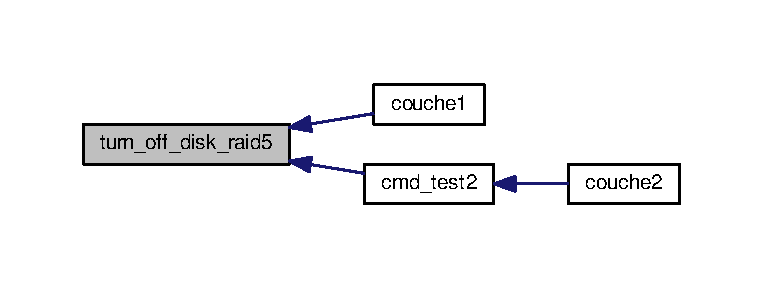
\includegraphics[width=350pt]{couche1_8h_a0f31c284e3b9461448ae2c5393a4c53f_icgraph}
\end{center}
\end{figure}
\mbox{\Hypertarget{couche1_8h_adb4607cf11ffed5c89fc0f4682bf6079}\label{couche1_8h_adb4607cf11ffed5c89fc0f4682bf6079}} 
\index{couche1.\+h@{couche1.\+h}!write\+\_\+block@{write\+\_\+block}}
\index{write\+\_\+block@{write\+\_\+block}!couche1.\+h@{couche1.\+h}}
\subsubsection{\texorpdfstring{write\+\_\+block()}{write\_block()}}
{\footnotesize\ttfamily void write\+\_\+block (\begin{DoxyParamCaption}\item[{\hyperlink{raid__defines_8h_ab22cb9a2c3c081d95bd06c65d6716686}{virtual\+\_\+disk\+\_\+t} $\ast$}]{R\+A\+I\+D5,  }\item[{\hyperlink{raid__defines_8h_a9497df9c1d65b018066a9760da7be4e6}{block\+\_\+t} $\ast$}]{entrant,  }\item[{\hyperlink{raid__defines_8h_a91ad9478d81a7aaf2593e8d9c3d06a14}{uint}}]{pos,  }\item[{int}]{id\+Disk }\end{DoxyParamCaption})}



Ecrit un bloc à la position pos sur le disque. 


\begin{DoxyParams}{Parameters}
{\em virtual\+\_\+disk\+\_\+t} & \\
\hline
{\em block\+\_\+t} & (à ecrire) \\
\hline
{\em uint} & (position à laquelle on ecrit) \\
\hline
{\em integer} & (n° disk) \\
\hline
\end{DoxyParams}
\begin{DoxyReturn}{Returns}
void 
\end{DoxyReturn}


Definition at line 112 of file couche1.\+c.

Here is the caller graph for this function\+:
\nopagebreak
\begin{figure}[H]
\begin{center}
\leavevmode
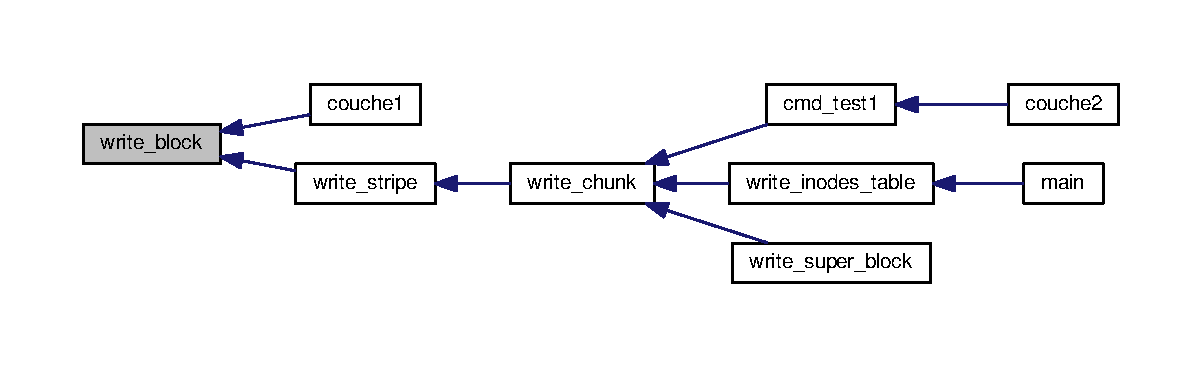
\includegraphics[width=350pt]{couche1_8h_adb4607cf11ffed5c89fc0f4682bf6079_icgraph}
\end{center}
\end{figure}
\mbox{\Hypertarget{couche1_8h_a69d295ba0ccd1a14fbc7ef4dd2c3a5c9}\label{couche1_8h_a69d295ba0ccd1a14fbc7ef4dd2c3a5c9}} 
\index{couche1.\+h@{couche1.\+h}!xorbl@{xorbl}}
\index{xorbl@{xorbl}!couche1.\+h@{couche1.\+h}}
\subsubsection{\texorpdfstring{xorbl()}{xorbl()}}
{\footnotesize\ttfamily void xorbl (\begin{DoxyParamCaption}\item[{\hyperlink{raid__defines_8h_a9497df9c1d65b018066a9760da7be4e6}{block\+\_\+t} $\ast$}]{xa,  }\item[{\hyperlink{raid__defines_8h_a9497df9c1d65b018066a9760da7be4e6}{block\+\_\+t} $\ast$}]{xb,  }\item[{\hyperlink{raid__defines_8h_a9497df9c1d65b018066a9760da7be4e6}{block\+\_\+t} $\ast$}]{destination }\end{DoxyParamCaption})}



Definition at line 141 of file couche1.\+c.

Here is the caller graph for this function\+:
\nopagebreak
\begin{figure}[H]
\begin{center}
\leavevmode
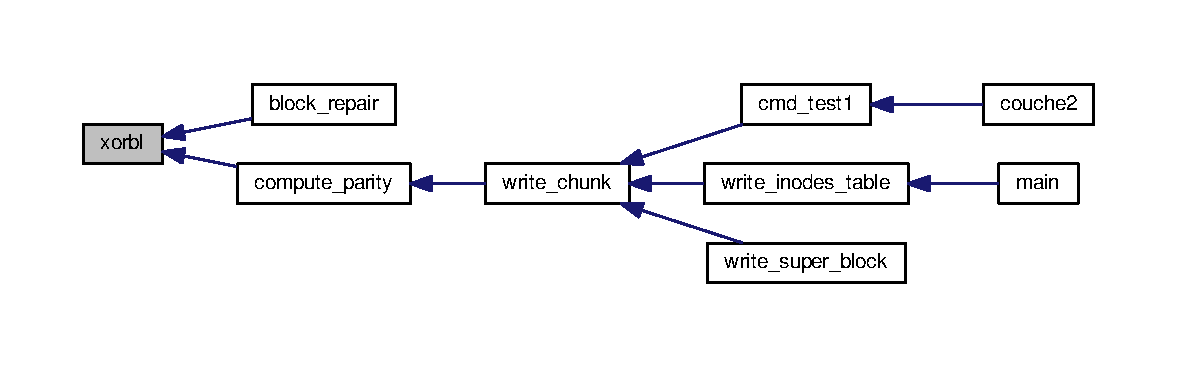
\includegraphics[width=350pt]{couche1_8h_a69d295ba0ccd1a14fbc7ef4dd2c3a5c9_icgraph}
\end{center}
\end{figure}

\hypertarget{couche2_8c}{}\section{couche2.\+c File Reference}
\label{couche2_8c}\index{couche2.\+c@{couche2.\+c}}


Programme couche2 du raid5.  


{\ttfamily \#include \char`\"{}couche1.\+h\char`\"{}}\newline
{\ttfamily \#include \char`\"{}couche2.\+h\char`\"{}}\newline
{\ttfamily \#include $<$stdlib.\+h$>$}\newline
{\ttfamily \#include $<$math.\+h$>$}\newline
Include dependency graph for couche2.\+c\+:
\nopagebreak
\begin{figure}[H]
\begin{center}
\leavevmode
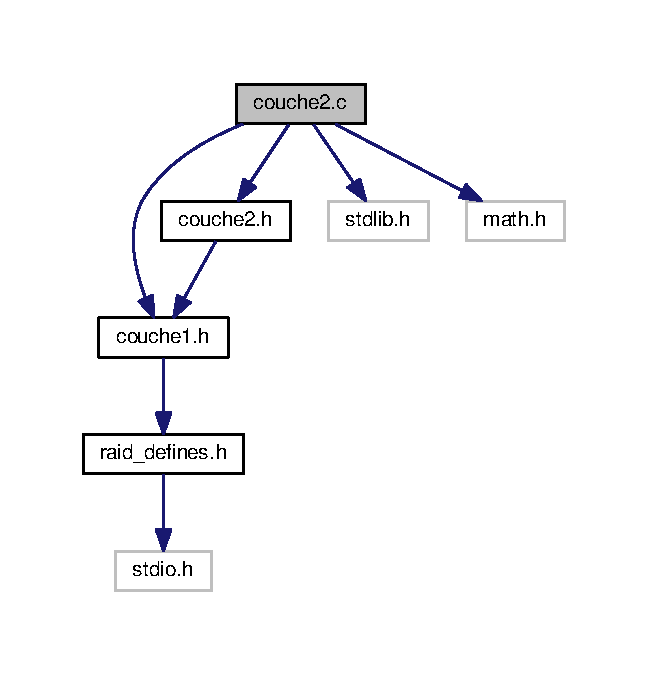
\includegraphics[width=311pt]{couche2_8c__incl}
\end{center}
\end{figure}
\subsection*{Functions}
\begin{DoxyCompactItemize}
\item 
int \hyperlink{couche2_8c_a3e5eab04f9ea03705105756c7b8c0782}{compute\+\_\+nstripe} (\hyperlink{raid__defines_8h_ab22cb9a2c3c081d95bd06c65d6716686}{virtual\+\_\+disk\+\_\+t} $\ast$\hyperlink{trash_8c_aa32bee7663041ae13a36afeae68a3f14}{r5\+Disk}, int nblocks)
\begin{DoxyCompactList}\small\item\em Retourne le nombre de bandes necessaires pour écrire n blocs. \end{DoxyCompactList}\item 
\hyperlink{raid__defines_8h_a9497df9c1d65b018066a9760da7be4e6}{block\+\_\+t} \hyperlink{couche2_8c_a9e6de3169d502aae6d8117e1e6ab03a0}{compute\+\_\+parity} (\hyperlink{raid__defines_8h_ab22cb9a2c3c081d95bd06c65d6716686}{virtual\+\_\+disk\+\_\+t} $\ast$r5, \hyperlink{raid__defines_8h_acfaa25ade17f36b058f738bded61819a}{stripe\+\_\+t} $\ast$tocompute, int indice\+\_\+parite)
\begin{DoxyCompactList}\small\item\em Calcule le bloc de parité d\textquotesingle{}une stripe. \end{DoxyCompactList}\item 
int \hyperlink{couche2_8c_a70860f329dcd21100a6648089f864ed0}{compute\+\_\+parity\+\_\+index} (\hyperlink{raid__defines_8h_ab22cb9a2c3c081d95bd06c65d6716686}{virtual\+\_\+disk\+\_\+t} $\ast$r5, int numbd)
\begin{DoxyCompactList}\small\item\em Calcule la position du block de parité d\textquotesingle{}une stripe. \end{DoxyCompactList}\item 
void \hyperlink{couche2_8c_a5033c8eea4a4da6a76284e361f13240d}{write\+\_\+stripe} (\hyperlink{raid__defines_8h_ab22cb9a2c3c081d95bd06c65d6716686}{virtual\+\_\+disk\+\_\+t} $\ast$r5, \hyperlink{raid__defines_8h_acfaa25ade17f36b058f738bded61819a}{stripe\+\_\+t} $\ast$ecrire, \hyperlink{raid__defines_8h_a91ad9478d81a7aaf2593e8d9c3d06a14}{uint} pos)
\begin{DoxyCompactList}\small\item\em Ecrit une stripe a la position passée en argument sur le raid passé en argument. \end{DoxyCompactList}\item 
\hyperlink{raid__defines_8h_acfaa25ade17f36b058f738bded61819a}{stripe\+\_\+t} $\ast$ \hyperlink{couche2_8c_ab6170c9cc6975d296a0bccfea207d415}{init\+\_\+bande} (\hyperlink{raid__defines_8h_ab22cb9a2c3c081d95bd06c65d6716686}{virtual\+\_\+disk\+\_\+t} $\ast$r5)
\item 
void \hyperlink{couche2_8c_adf66b9197c93775a6c1dba723ba92a07}{delete\+\_\+bande} (\hyperlink{raid__defines_8h_acfaa25ade17f36b058f738bded61819a}{stripe\+\_\+t} $\ast$$\ast$bande)
\begin{DoxyCompactList}\small\item\em Libere la mémoir réservée par une bande. \end{DoxyCompactList}\item 
void \hyperlink{couche2_8c_a2fa67e5d44f8746a06cc56ef2876c45e}{print\+\_\+stripe} (\hyperlink{raid__defines_8h_ab22cb9a2c3c081d95bd06c65d6716686}{virtual\+\_\+disk\+\_\+t} $\ast$r5, \hyperlink{raid__defines_8h_acfaa25ade17f36b058f738bded61819a}{stripe\+\_\+t} $\ast$stripe)
\begin{DoxyCompactList}\small\item\em Affiche une bande. \end{DoxyCompactList}\item 
void \hyperlink{couche2_8c_a7ba1127dd9f6b03cbef1c8974790d3c6}{write\+\_\+chunk} (\hyperlink{raid__defines_8h_ab22cb9a2c3c081d95bd06c65d6716686}{virtual\+\_\+disk\+\_\+t} $\ast$r5, char $\ast$buffer, int n, \hyperlink{raid__defines_8h_a91ad9478d81a7aaf2593e8d9c3d06a14}{uint} start\+Block)
\begin{DoxyCompactList}\small\item\em Ecrit une stripe a la position passée en argument sur le raid passé en argument. \end{DoxyCompactList}\item 
int \hyperlink{couche2_8c_a37df3c8400bc0d4673471a52757d023a}{afficher\+\_\+raid\+\_\+hexa} (\hyperlink{raid__defines_8h_ab22cb9a2c3c081d95bd06c65d6716686}{virtual\+\_\+disk\+\_\+t} $\ast$r5)
\item 
int \hyperlink{couche2_8c_a5e216cfa058baf4a67b6fc96773fe095}{afficher\+\_\+raid\+\_\+decimal} (\hyperlink{raid__defines_8h_ab22cb9a2c3c081d95bd06c65d6716686}{virtual\+\_\+disk\+\_\+t} $\ast$r5)
\begin{DoxyCompactList}\small\item\em affiche les disques du raid en valeurs décimales \end{DoxyCompactList}\item 
void \hyperlink{couche2_8c_abc2b7fd9807ede9a34e0d2bea6e9521c}{cmd\+\_\+test1} (\hyperlink{raid__defines_8h_ab22cb9a2c3c081d95bd06c65d6716686}{virtual\+\_\+disk\+\_\+t} $\ast$r5)
\begin{DoxyCompactList}\small\item\em fonction de test pour write\+\_\+chunk \end{DoxyCompactList}\item 
int \hyperlink{couche2_8c_aea9498cb46077bb21181922c96e8329f}{read\+\_\+stripe} (\hyperlink{raid__defines_8h_ab22cb9a2c3c081d95bd06c65d6716686}{virtual\+\_\+disk\+\_\+t} $\ast$r5, \hyperlink{raid__defines_8h_acfaa25ade17f36b058f738bded61819a}{stripe\+\_\+t} $\ast$lire, \hyperlink{raid__defines_8h_a91ad9478d81a7aaf2593e8d9c3d06a14}{uint} pos)
\begin{DoxyCompactList}\small\item\em Lis une bande a partir de la position passée en parametre. \end{DoxyCompactList}\item 
void \hyperlink{couche2_8c_a2c76b4c3607585f36f7e7653fb96d633}{cmd\+\_\+test2} (\hyperlink{raid__defines_8h_ab22cb9a2c3c081d95bd06c65d6716686}{virtual\+\_\+disk\+\_\+t} $\ast$r5)
\begin{DoxyCompactList}\small\item\em Fonction de test pour read\+\_\+chunk. \end{DoxyCompactList}\item 
int \hyperlink{couche2_8c_a1365b1597af91528776b50b5bc418a08}{compute\+\_\+num\+\_\+bande} (\hyperlink{raid__defines_8h_ab22cb9a2c3c081d95bd06c65d6716686}{virtual\+\_\+disk\+\_\+t} $\ast$r5, int nbloc)
\begin{DoxyCompactList}\small\item\em Fonction retournant le num de la bande actuelle. \end{DoxyCompactList}\item 
char $\ast$ \hyperlink{couche2_8c_a1868b67f893921ee137623a23e4b6dd8}{read\+\_\+chunk} (\hyperlink{raid__defines_8h_ab22cb9a2c3c081d95bd06c65d6716686}{virtual\+\_\+disk\+\_\+t} $\ast$r5, \hyperlink{raid__defines_8h_a91ad9478d81a7aaf2593e8d9c3d06a14}{uint} start\+\_\+block, int n)
\begin{DoxyCompactList}\small\item\em Fonction de lecture de tableau de char. \end{DoxyCompactList}\item 
int \hyperlink{couche2_8c_a38818187df03f330b062dcc1b3cf78df}{couche2} (void)
\end{DoxyCompactItemize}


\subsection{Detailed Description}
Programme couche2 du raid5. 

\begin{DoxyAuthor}{Author}
Groupe14 
\end{DoxyAuthor}
\begin{DoxyVersion}{Version}
0.\+1 
\end{DoxyVersion}
\begin{DoxyDate}{Date}
24 fevrier 2019
\end{DoxyDate}
Programme de la couche 2 du raid5. 

\subsection{Function Documentation}
\mbox{\Hypertarget{couche2_8c_a5e216cfa058baf4a67b6fc96773fe095}\label{couche2_8c_a5e216cfa058baf4a67b6fc96773fe095}} 
\index{couche2.\+c@{couche2.\+c}!afficher\+\_\+raid\+\_\+decimal@{afficher\+\_\+raid\+\_\+decimal}}
\index{afficher\+\_\+raid\+\_\+decimal@{afficher\+\_\+raid\+\_\+decimal}!couche2.\+c@{couche2.\+c}}
\subsubsection{\texorpdfstring{afficher\+\_\+raid\+\_\+decimal()}{afficher\_raid\_decimal()}}
{\footnotesize\ttfamily int afficher\+\_\+raid\+\_\+decimal (\begin{DoxyParamCaption}\item[{\hyperlink{raid__defines_8h_ab22cb9a2c3c081d95bd06c65d6716686}{virtual\+\_\+disk\+\_\+t} $\ast$}]{r5 }\end{DoxyParamCaption})}



affiche les disques du raid en valeurs décimales 


\begin{DoxyParams}{Parameters}
{\em } & virtual\+\_\+disk\+\_\+t $\ast$ \\
\hline
\end{DoxyParams}
\begin{DoxyReturn}{Returns}
int 
\end{DoxyReturn}


Definition at line 172 of file couche2.\+c.

Here is the call graph for this function\+:
\nopagebreak
\begin{figure}[H]
\begin{center}
\leavevmode
\includegraphics[width=350pt]{couche2_8c_a5e216cfa058baf4a67b6fc96773fe095_cgraph}
\end{center}
\end{figure}
Here is the caller graph for this function\+:
\nopagebreak
\begin{figure}[H]
\begin{center}
\leavevmode
\includegraphics[width=350pt]{couche2_8c_a5e216cfa058baf4a67b6fc96773fe095_icgraph}
\end{center}
\end{figure}
\mbox{\Hypertarget{couche2_8c_a37df3c8400bc0d4673471a52757d023a}\label{couche2_8c_a37df3c8400bc0d4673471a52757d023a}} 
\index{couche2.\+c@{couche2.\+c}!afficher\+\_\+raid\+\_\+hexa@{afficher\+\_\+raid\+\_\+hexa}}
\index{afficher\+\_\+raid\+\_\+hexa@{afficher\+\_\+raid\+\_\+hexa}!couche2.\+c@{couche2.\+c}}
\subsubsection{\texorpdfstring{afficher\+\_\+raid\+\_\+hexa()}{afficher\_raid\_hexa()}}
{\footnotesize\ttfamily int afficher\+\_\+raid\+\_\+hexa (\begin{DoxyParamCaption}\item[{\hyperlink{raid__defines_8h_ab22cb9a2c3c081d95bd06c65d6716686}{virtual\+\_\+disk\+\_\+t} $\ast$}]{r5 }\end{DoxyParamCaption})}



Definition at line 150 of file couche2.\+c.

Here is the call graph for this function\+:
\nopagebreak
\begin{figure}[H]
\begin{center}
\leavevmode
\includegraphics[width=350pt]{couche2_8c_a37df3c8400bc0d4673471a52757d023a_cgraph}
\end{center}
\end{figure}
Here is the caller graph for this function\+:
\nopagebreak
\begin{figure}[H]
\begin{center}
\leavevmode
\includegraphics[width=350pt]{couche2_8c_a37df3c8400bc0d4673471a52757d023a_icgraph}
\end{center}
\end{figure}
\mbox{\Hypertarget{couche2_8c_abc2b7fd9807ede9a34e0d2bea6e9521c}\label{couche2_8c_abc2b7fd9807ede9a34e0d2bea6e9521c}} 
\index{couche2.\+c@{couche2.\+c}!cmd\+\_\+test1@{cmd\+\_\+test1}}
\index{cmd\+\_\+test1@{cmd\+\_\+test1}!couche2.\+c@{couche2.\+c}}
\subsubsection{\texorpdfstring{cmd\+\_\+test1()}{cmd\_test1()}}
{\footnotesize\ttfamily void cmd\+\_\+test1 (\begin{DoxyParamCaption}\item[{\hyperlink{raid__defines_8h_ab22cb9a2c3c081d95bd06c65d6716686}{virtual\+\_\+disk\+\_\+t} $\ast$}]{r5 }\end{DoxyParamCaption})}



fonction de test pour write\+\_\+chunk 


\begin{DoxyParams}{Parameters}
{\em virtual\+\_\+disk\+\_\+t} & $\ast$ \\
\hline
\end{DoxyParams}


Definition at line 194 of file couche2.\+c.

Here is the call graph for this function\+:
\nopagebreak
\begin{figure}[H]
\begin{center}
\leavevmode
\includegraphics[width=350pt]{couche2_8c_abc2b7fd9807ede9a34e0d2bea6e9521c_cgraph}
\end{center}
\end{figure}
Here is the caller graph for this function\+:
\nopagebreak
\begin{figure}[H]
\begin{center}
\leavevmode
\includegraphics[width=231pt]{couche2_8c_abc2b7fd9807ede9a34e0d2bea6e9521c_icgraph}
\end{center}
\end{figure}
\mbox{\Hypertarget{couche2_8c_a2c76b4c3607585f36f7e7653fb96d633}\label{couche2_8c_a2c76b4c3607585f36f7e7653fb96d633}} 
\index{couche2.\+c@{couche2.\+c}!cmd\+\_\+test2@{cmd\+\_\+test2}}
\index{cmd\+\_\+test2@{cmd\+\_\+test2}!couche2.\+c@{couche2.\+c}}
\subsubsection{\texorpdfstring{cmd\+\_\+test2()}{cmd\_test2()}}
{\footnotesize\ttfamily void cmd\+\_\+test2 (\begin{DoxyParamCaption}\item[{\hyperlink{raid__defines_8h_ab22cb9a2c3c081d95bd06c65d6716686}{virtual\+\_\+disk\+\_\+t} $\ast$}]{r5 }\end{DoxyParamCaption})}



Fonction de test pour read\+\_\+chunk. 


\begin{DoxyParams}{Parameters}
{\em } & virtual\+\_\+disk\+\_\+t $\ast$ \\
\hline
\end{DoxyParams}
\begin{DoxyReturn}{Returns}
void 
\end{DoxyReturn}


Definition at line 228 of file couche2.\+c.

Here is the call graph for this function\+:
\nopagebreak
\begin{figure}[H]
\begin{center}
\leavevmode
\includegraphics[width=350pt]{couche2_8c_a2c76b4c3607585f36f7e7653fb96d633_cgraph}
\end{center}
\end{figure}
Here is the caller graph for this function\+:
\nopagebreak
\begin{figure}[H]
\begin{center}
\leavevmode
\includegraphics[width=231pt]{couche2_8c_a2c76b4c3607585f36f7e7653fb96d633_icgraph}
\end{center}
\end{figure}
\mbox{\Hypertarget{couche2_8c_a3e5eab04f9ea03705105756c7b8c0782}\label{couche2_8c_a3e5eab04f9ea03705105756c7b8c0782}} 
\index{couche2.\+c@{couche2.\+c}!compute\+\_\+nstripe@{compute\+\_\+nstripe}}
\index{compute\+\_\+nstripe@{compute\+\_\+nstripe}!couche2.\+c@{couche2.\+c}}
\subsubsection{\texorpdfstring{compute\+\_\+nstripe()}{compute\_nstripe()}}
{\footnotesize\ttfamily int compute\+\_\+nstripe (\begin{DoxyParamCaption}\item[{\hyperlink{raid__defines_8h_ab22cb9a2c3c081d95bd06c65d6716686}{virtual\+\_\+disk\+\_\+t} $\ast$}]{r5\+Disk,  }\item[{int}]{nblocks }\end{DoxyParamCaption})}



Retourne le nombre de bandes necessaires pour écrire n blocs. 


\begin{DoxyParams}{Parameters}
{\em } & Nombre de blocs (int) \\
\hline
\end{DoxyParams}
\begin{DoxyReturn}{Returns}
Nombre de bandes (int) 
\end{DoxyReturn}


Definition at line 23 of file couche2.\+c.

Here is the caller graph for this function\+:
\nopagebreak
\begin{figure}[H]
\begin{center}
\leavevmode
\includegraphics[width=350pt]{couche2_8c_a3e5eab04f9ea03705105756c7b8c0782_icgraph}
\end{center}
\end{figure}
\mbox{\Hypertarget{couche2_8c_a1365b1597af91528776b50b5bc418a08}\label{couche2_8c_a1365b1597af91528776b50b5bc418a08}} 
\index{couche2.\+c@{couche2.\+c}!compute\+\_\+num\+\_\+bande@{compute\+\_\+num\+\_\+bande}}
\index{compute\+\_\+num\+\_\+bande@{compute\+\_\+num\+\_\+bande}!couche2.\+c@{couche2.\+c}}
\subsubsection{\texorpdfstring{compute\+\_\+num\+\_\+bande()}{compute\_num\_bande()}}
{\footnotesize\ttfamily int compute\+\_\+num\+\_\+bande (\begin{DoxyParamCaption}\item[{\hyperlink{raid__defines_8h_ab22cb9a2c3c081d95bd06c65d6716686}{virtual\+\_\+disk\+\_\+t} $\ast$}]{r5,  }\item[{int}]{nbloc }\end{DoxyParamCaption})}



Fonction retournant le num de la bande actuelle. 


\begin{DoxyParams}{Parameters}
{\em } & virtual\+\_\+disk\+\_\+t $\ast$ le systeme \\
\hline
{\em } & int le numéro du block actuel \\
\hline
\end{DoxyParams}
\begin{DoxyReturn}{Returns}
\+: int le numero de la bande 
\end{DoxyReturn}


Definition at line 242 of file couche2.\+c.

Here is the caller graph for this function\+:
\nopagebreak
\begin{figure}[H]
\begin{center}
\leavevmode
\includegraphics[width=350pt]{couche2_8c_a1365b1597af91528776b50b5bc418a08_icgraph}
\end{center}
\end{figure}
\mbox{\Hypertarget{couche2_8c_a9e6de3169d502aae6d8117e1e6ab03a0}\label{couche2_8c_a9e6de3169d502aae6d8117e1e6ab03a0}} 
\index{couche2.\+c@{couche2.\+c}!compute\+\_\+parity@{compute\+\_\+parity}}
\index{compute\+\_\+parity@{compute\+\_\+parity}!couche2.\+c@{couche2.\+c}}
\subsubsection{\texorpdfstring{compute\+\_\+parity()}{compute\_parity()}}
{\footnotesize\ttfamily \hyperlink{raid__defines_8h_a9497df9c1d65b018066a9760da7be4e6}{block\+\_\+t} compute\+\_\+parity (\begin{DoxyParamCaption}\item[{\hyperlink{raid__defines_8h_ab22cb9a2c3c081d95bd06c65d6716686}{virtual\+\_\+disk\+\_\+t} $\ast$}]{r5,  }\item[{\hyperlink{raid__defines_8h_acfaa25ade17f36b058f738bded61819a}{stripe\+\_\+t} $\ast$}]{tocompute,  }\item[{int}]{indice\+\_\+parite }\end{DoxyParamCaption})}



Calcule le bloc de parité d\textquotesingle{}une stripe. 


\begin{DoxyParams}{Parameters}
{\em } & virtual\+\_\+disk\+\_\+t $\ast$, stripe\+\_\+t $\ast$,int \\
\hline
\end{DoxyParams}
\begin{DoxyReturn}{Returns}
block\+\_\+t 
\end{DoxyReturn}


Definition at line 35 of file couche2.\+c.

Here is the call graph for this function\+:
\nopagebreak
\begin{figure}[H]
\begin{center}
\leavevmode
\includegraphics[width=237pt]{couche2_8c_a9e6de3169d502aae6d8117e1e6ab03a0_cgraph}
\end{center}
\end{figure}
Here is the caller graph for this function\+:
\nopagebreak
\begin{figure}[H]
\begin{center}
\leavevmode
\includegraphics[width=350pt]{couche2_8c_a9e6de3169d502aae6d8117e1e6ab03a0_icgraph}
\end{center}
\end{figure}
\mbox{\Hypertarget{couche2_8c_a70860f329dcd21100a6648089f864ed0}\label{couche2_8c_a70860f329dcd21100a6648089f864ed0}} 
\index{couche2.\+c@{couche2.\+c}!compute\+\_\+parity\+\_\+index@{compute\+\_\+parity\+\_\+index}}
\index{compute\+\_\+parity\+\_\+index@{compute\+\_\+parity\+\_\+index}!couche2.\+c@{couche2.\+c}}
\subsubsection{\texorpdfstring{compute\+\_\+parity\+\_\+index()}{compute\_parity\_index()}}
{\footnotesize\ttfamily int compute\+\_\+parity\+\_\+index (\begin{DoxyParamCaption}\item[{\hyperlink{raid__defines_8h_ab22cb9a2c3c081d95bd06c65d6716686}{virtual\+\_\+disk\+\_\+t} $\ast$}]{r5,  }\item[{int}]{numbd }\end{DoxyParamCaption})}



Calcule la position du block de parité d\textquotesingle{}une stripe. 


\begin{DoxyParams}{Parameters}
{\em } & virtual\+\_\+disk\+\_\+t , int numero de la bande dans la liste du raid \\
\hline
\end{DoxyParams}
\begin{DoxyReturn}{Returns}
int 
\end{DoxyReturn}


Definition at line 50 of file couche2.\+c.

Here is the caller graph for this function\+:
\nopagebreak
\begin{figure}[H]
\begin{center}
\leavevmode
\includegraphics[width=350pt]{couche2_8c_a70860f329dcd21100a6648089f864ed0_icgraph}
\end{center}
\end{figure}
\mbox{\Hypertarget{couche2_8c_a38818187df03f330b062dcc1b3cf78df}\label{couche2_8c_a38818187df03f330b062dcc1b3cf78df}} 
\index{couche2.\+c@{couche2.\+c}!couche2@{couche2}}
\index{couche2@{couche2}!couche2.\+c@{couche2.\+c}}
\subsubsection{\texorpdfstring{couche2()}{couche2()}}
{\footnotesize\ttfamily int couche2 (\begin{DoxyParamCaption}\item[{void}]{ }\end{DoxyParamCaption})}



Definition at line 278 of file couche2.\+c.

Here is the call graph for this function\+:
\nopagebreak
\begin{figure}[H]
\begin{center}
\leavevmode
\includegraphics[width=350pt]{couche2_8c_a38818187df03f330b062dcc1b3cf78df_cgraph}
\end{center}
\end{figure}
\mbox{\Hypertarget{couche2_8c_adf66b9197c93775a6c1dba723ba92a07}\label{couche2_8c_adf66b9197c93775a6c1dba723ba92a07}} 
\index{couche2.\+c@{couche2.\+c}!delete\+\_\+bande@{delete\+\_\+bande}}
\index{delete\+\_\+bande@{delete\+\_\+bande}!couche2.\+c@{couche2.\+c}}
\subsubsection{\texorpdfstring{delete\+\_\+bande()}{delete\_bande()}}
{\footnotesize\ttfamily void delete\+\_\+bande (\begin{DoxyParamCaption}\item[{\hyperlink{raid__defines_8h_acfaa25ade17f36b058f738bded61819a}{stripe\+\_\+t} $\ast$$\ast$}]{bande }\end{DoxyParamCaption})}



Libere la mémoir réservée par une bande. 


\begin{DoxyParams}{Parameters}
{\em } & stripe\+\_\+t $\ast$ \\
\hline
\end{DoxyParams}
\begin{DoxyReturn}{Returns}
void 
\end{DoxyReturn}


Definition at line 82 of file couche2.\+c.

Here is the caller graph for this function\+:
\nopagebreak
\begin{figure}[H]
\begin{center}
\leavevmode
\includegraphics[width=350pt]{couche2_8c_adf66b9197c93775a6c1dba723ba92a07_icgraph}
\end{center}
\end{figure}
\mbox{\Hypertarget{couche2_8c_ab6170c9cc6975d296a0bccfea207d415}\label{couche2_8c_ab6170c9cc6975d296a0bccfea207d415}} 
\index{couche2.\+c@{couche2.\+c}!init\+\_\+bande@{init\+\_\+bande}}
\index{init\+\_\+bande@{init\+\_\+bande}!couche2.\+c@{couche2.\+c}}
\subsubsection{\texorpdfstring{init\+\_\+bande()}{init\_bande()}}
{\footnotesize\ttfamily \hyperlink{raid__defines_8h_acfaa25ade17f36b058f738bded61819a}{stripe\+\_\+t}$\ast$ init\+\_\+bande (\begin{DoxyParamCaption}\item[{\hyperlink{raid__defines_8h_ab22cb9a2c3c081d95bd06c65d6716686}{virtual\+\_\+disk\+\_\+t} $\ast$}]{r5 }\end{DoxyParamCaption})}



Definition at line 70 of file couche2.\+c.

Here is the caller graph for this function\+:
\nopagebreak
\begin{figure}[H]
\begin{center}
\leavevmode
\includegraphics[width=350pt]{couche2_8c_ab6170c9cc6975d296a0bccfea207d415_icgraph}
\end{center}
\end{figure}
\mbox{\Hypertarget{couche2_8c_a2fa67e5d44f8746a06cc56ef2876c45e}\label{couche2_8c_a2fa67e5d44f8746a06cc56ef2876c45e}} 
\index{couche2.\+c@{couche2.\+c}!print\+\_\+stripe@{print\+\_\+stripe}}
\index{print\+\_\+stripe@{print\+\_\+stripe}!couche2.\+c@{couche2.\+c}}
\subsubsection{\texorpdfstring{print\+\_\+stripe()}{print\_stripe()}}
{\footnotesize\ttfamily void print\+\_\+stripe (\begin{DoxyParamCaption}\item[{\hyperlink{raid__defines_8h_ab22cb9a2c3c081d95bd06c65d6716686}{virtual\+\_\+disk\+\_\+t} $\ast$}]{r5,  }\item[{\hyperlink{raid__defines_8h_acfaa25ade17f36b058f738bded61819a}{stripe\+\_\+t} $\ast$}]{stripe }\end{DoxyParamCaption})}



Affiche une bande. 


\begin{DoxyParams}{Parameters}
{\em } & virtual\+\_\+disk\+\_\+t ,stripe\+\_\+t \\
\hline
\end{DoxyParams}
\begin{DoxyReturn}{Returns}
void 
\end{DoxyReturn}


Definition at line 93 of file couche2.\+c.

Here is the call graph for this function\+:
\nopagebreak
\begin{figure}[H]
\begin{center}
\leavevmode
\includegraphics[width=259pt]{couche2_8c_a2fa67e5d44f8746a06cc56ef2876c45e_cgraph}
\end{center}
\end{figure}
\mbox{\Hypertarget{couche2_8c_a1868b67f893921ee137623a23e4b6dd8}\label{couche2_8c_a1868b67f893921ee137623a23e4b6dd8}} 
\index{couche2.\+c@{couche2.\+c}!read\+\_\+chunk@{read\+\_\+chunk}}
\index{read\+\_\+chunk@{read\+\_\+chunk}!couche2.\+c@{couche2.\+c}}
\subsubsection{\texorpdfstring{read\+\_\+chunk()}{read\_chunk()}}
{\footnotesize\ttfamily char$\ast$ read\+\_\+chunk (\begin{DoxyParamCaption}\item[{\hyperlink{raid__defines_8h_ab22cb9a2c3c081d95bd06c65d6716686}{virtual\+\_\+disk\+\_\+t} $\ast$}]{r5,  }\item[{\hyperlink{raid__defines_8h_a91ad9478d81a7aaf2593e8d9c3d06a14}{uint}}]{start\+\_\+block,  }\item[{int}]{n }\end{DoxyParamCaption})}



Fonction de lecture de tableau de char. 


\begin{DoxyParams}{Parameters}
{\em } & virtual\+\_\+disk\+\_\+t $\ast$ , uint , int \\
\hline
\end{DoxyParams}
\begin{DoxyReturn}{Returns}
char $\ast$ 
\end{DoxyReturn}


Definition at line 251 of file couche2.\+c.

Here is the call graph for this function\+:
\nopagebreak
\begin{figure}[H]
\begin{center}
\leavevmode
\includegraphics[width=295pt]{couche2_8c_a1868b67f893921ee137623a23e4b6dd8_cgraph}
\end{center}
\end{figure}
Here is the caller graph for this function\+:
\nopagebreak
\begin{figure}[H]
\begin{center}
\leavevmode
\includegraphics[width=334pt]{couche2_8c_a1868b67f893921ee137623a23e4b6dd8_icgraph}
\end{center}
\end{figure}
\mbox{\Hypertarget{couche2_8c_aea9498cb46077bb21181922c96e8329f}\label{couche2_8c_aea9498cb46077bb21181922c96e8329f}} 
\index{couche2.\+c@{couche2.\+c}!read\+\_\+stripe@{read\+\_\+stripe}}
\index{read\+\_\+stripe@{read\+\_\+stripe}!couche2.\+c@{couche2.\+c}}
\subsubsection{\texorpdfstring{read\+\_\+stripe()}{read\_stripe()}}
{\footnotesize\ttfamily int read\+\_\+stripe (\begin{DoxyParamCaption}\item[{\hyperlink{raid__defines_8h_ab22cb9a2c3c081d95bd06c65d6716686}{virtual\+\_\+disk\+\_\+t} $\ast$}]{r5,  }\item[{\hyperlink{raid__defines_8h_acfaa25ade17f36b058f738bded61819a}{stripe\+\_\+t} $\ast$}]{lire,  }\item[{\hyperlink{raid__defines_8h_a91ad9478d81a7aaf2593e8d9c3d06a14}{uint}}]{pos }\end{DoxyParamCaption})}



Lis une bande a partir de la position passée en parametre. 


\begin{DoxyParams}{Parameters}
{\em } & virtual\+\_\+disk\+\_\+t $\ast$,stripe\+\_\+t $\ast$, uint \\
\hline
\end{DoxyParams}
\begin{DoxyReturn}{Returns}
int 
\end{DoxyReturn}


Definition at line 211 of file couche2.\+c.

Here is the call graph for this function\+:
\nopagebreak
\begin{figure}[H]
\begin{center}
\leavevmode
\includegraphics[width=245pt]{couche2_8c_aea9498cb46077bb21181922c96e8329f_cgraph}
\end{center}
\end{figure}
Here is the caller graph for this function\+:
\nopagebreak
\begin{figure}[H]
\begin{center}
\leavevmode
\includegraphics[width=350pt]{couche2_8c_aea9498cb46077bb21181922c96e8329f_icgraph}
\end{center}
\end{figure}
\mbox{\Hypertarget{couche2_8c_a7ba1127dd9f6b03cbef1c8974790d3c6}\label{couche2_8c_a7ba1127dd9f6b03cbef1c8974790d3c6}} 
\index{couche2.\+c@{couche2.\+c}!write\+\_\+chunk@{write\+\_\+chunk}}
\index{write\+\_\+chunk@{write\+\_\+chunk}!couche2.\+c@{couche2.\+c}}
\subsubsection{\texorpdfstring{write\+\_\+chunk()}{write\_chunk()}}
{\footnotesize\ttfamily void write\+\_\+chunk (\begin{DoxyParamCaption}\item[{\hyperlink{raid__defines_8h_ab22cb9a2c3c081d95bd06c65d6716686}{virtual\+\_\+disk\+\_\+t} $\ast$}]{r5,  }\item[{char $\ast$}]{buffer,  }\item[{int}]{n,  }\item[{\hyperlink{raid__defines_8h_a91ad9478d81a7aaf2593e8d9c3d06a14}{uint}}]{start\+Block }\end{DoxyParamCaption})}



Ecrit une stripe a la position passée en argument sur le raid passé en argument. 


\begin{DoxyParams}{Parameters}
{\em } & virtual\+\_\+disk\+\_\+t ,stripe\+\_\+t ,int \\
\hline
\end{DoxyParams}
\begin{DoxyReturn}{Returns}
void 
\end{DoxyReturn}


Definition at line 112 of file couche2.\+c.

Here is the call graph for this function\+:
\nopagebreak
\begin{figure}[H]
\begin{center}
\leavevmode
\includegraphics[width=350pt]{couche2_8c_a7ba1127dd9f6b03cbef1c8974790d3c6_cgraph}
\end{center}
\end{figure}
Here is the caller graph for this function\+:
\nopagebreak
\begin{figure}[H]
\begin{center}
\leavevmode
\includegraphics[width=350pt]{couche2_8c_a7ba1127dd9f6b03cbef1c8974790d3c6_icgraph}
\end{center}
\end{figure}
\mbox{\Hypertarget{couche2_8c_a5033c8eea4a4da6a76284e361f13240d}\label{couche2_8c_a5033c8eea4a4da6a76284e361f13240d}} 
\index{couche2.\+c@{couche2.\+c}!write\+\_\+stripe@{write\+\_\+stripe}}
\index{write\+\_\+stripe@{write\+\_\+stripe}!couche2.\+c@{couche2.\+c}}
\subsubsection{\texorpdfstring{write\+\_\+stripe()}{write\_stripe()}}
{\footnotesize\ttfamily void write\+\_\+stripe (\begin{DoxyParamCaption}\item[{\hyperlink{raid__defines_8h_ab22cb9a2c3c081d95bd06c65d6716686}{virtual\+\_\+disk\+\_\+t} $\ast$}]{r5,  }\item[{\hyperlink{raid__defines_8h_acfaa25ade17f36b058f738bded61819a}{stripe\+\_\+t} $\ast$}]{ecrire,  }\item[{\hyperlink{raid__defines_8h_a91ad9478d81a7aaf2593e8d9c3d06a14}{uint}}]{pos }\end{DoxyParamCaption})}



Ecrit une stripe a la position passée en argument sur le raid passé en argument. 


\begin{DoxyParams}{Parameters}
{\em } & virtual\+\_\+disk\+\_\+t ,stripe\+\_\+t ,int \\
\hline
\end{DoxyParams}
\begin{DoxyReturn}{Returns}
void 
\end{DoxyReturn}


Definition at line 63 of file couche2.\+c.

Here is the call graph for this function\+:
\nopagebreak
\begin{figure}[H]
\begin{center}
\leavevmode
\includegraphics[width=249pt]{couche2_8c_a5033c8eea4a4da6a76284e361f13240d_cgraph}
\end{center}
\end{figure}
Here is the caller graph for this function\+:
\nopagebreak
\begin{figure}[H]
\begin{center}
\leavevmode
\includegraphics[width=350pt]{couche2_8c_a5033c8eea4a4da6a76284e361f13240d_icgraph}
\end{center}
\end{figure}

\hypertarget{couche2_8h}{}\section{couche2.\+h File Reference}
\label{couche2_8h}\index{couche2.\+h@{couche2.\+h}}
{\ttfamily \#include \char`\"{}couche1.\+h\char`\"{}}\newline
Include dependency graph for couche2.\+h\+:
\nopagebreak
\begin{figure}[H]
\begin{center}
\leavevmode
\includegraphics[width=157pt]{couche2_8h__incl}
\end{center}
\end{figure}
This graph shows which files directly or indirectly include this file\+:
\nopagebreak
\begin{figure}[H]
\begin{center}
\leavevmode
\includegraphics[width=251pt]{couche2_8h__dep__incl}
\end{center}
\end{figure}
\subsection*{Functions}
\begin{DoxyCompactItemize}
\item 
int \hyperlink{couche2_8h_a3e5eab04f9ea03705105756c7b8c0782}{compute\+\_\+nstripe} (\hyperlink{raid__defines_8h_ab22cb9a2c3c081d95bd06c65d6716686}{virtual\+\_\+disk\+\_\+t} $\ast$\hyperlink{trash_8c_aa32bee7663041ae13a36afeae68a3f14}{r5\+Disk}, int nblocks)
\begin{DoxyCompactList}\small\item\em Retourne le nombre de bandes necessaires pour écrire n blocs. \end{DoxyCompactList}\item 
\hyperlink{raid__defines_8h_a9497df9c1d65b018066a9760da7be4e6}{block\+\_\+t} \hyperlink{couche2_8h_a9e6de3169d502aae6d8117e1e6ab03a0}{compute\+\_\+parity} (\hyperlink{raid__defines_8h_ab22cb9a2c3c081d95bd06c65d6716686}{virtual\+\_\+disk\+\_\+t} $\ast$r5, \hyperlink{raid__defines_8h_acfaa25ade17f36b058f738bded61819a}{stripe\+\_\+t} $\ast$tocompute, int indice\+\_\+parite)
\begin{DoxyCompactList}\small\item\em Calcule le bloc de parité d\textquotesingle{}une stripe. \end{DoxyCompactList}\item 
int \hyperlink{couche2_8h_a70860f329dcd21100a6648089f864ed0}{compute\+\_\+parity\+\_\+index} (\hyperlink{raid__defines_8h_ab22cb9a2c3c081d95bd06c65d6716686}{virtual\+\_\+disk\+\_\+t} $\ast$r5, int numbd)
\begin{DoxyCompactList}\small\item\em Calcule la position du block de parité d\textquotesingle{}une stripe. \end{DoxyCompactList}\item 
void \hyperlink{couche2_8h_a5033c8eea4a4da6a76284e361f13240d}{write\+\_\+stripe} (\hyperlink{raid__defines_8h_ab22cb9a2c3c081d95bd06c65d6716686}{virtual\+\_\+disk\+\_\+t} $\ast$r5, \hyperlink{raid__defines_8h_acfaa25ade17f36b058f738bded61819a}{stripe\+\_\+t} $\ast$ecrire, \hyperlink{raid__defines_8h_a91ad9478d81a7aaf2593e8d9c3d06a14}{uint} pos)
\begin{DoxyCompactList}\small\item\em Ecrit une stripe a la position passée en argument sur le raid passé en argument. \end{DoxyCompactList}\item 
void \hyperlink{couche2_8h_a7ba1127dd9f6b03cbef1c8974790d3c6}{write\+\_\+chunk} (\hyperlink{raid__defines_8h_ab22cb9a2c3c081d95bd06c65d6716686}{virtual\+\_\+disk\+\_\+t} $\ast$r5, char $\ast$buffer, int n, \hyperlink{raid__defines_8h_a91ad9478d81a7aaf2593e8d9c3d06a14}{uint} start\+Block)
\begin{DoxyCompactList}\small\item\em Ecrit une stripe a la position passée en argument sur le raid passé en argument. \end{DoxyCompactList}\item 
char $\ast$ \hyperlink{couche2_8h_a1868b67f893921ee137623a23e4b6dd8}{read\+\_\+chunk} (\hyperlink{raid__defines_8h_ab22cb9a2c3c081d95bd06c65d6716686}{virtual\+\_\+disk\+\_\+t} $\ast$r5, \hyperlink{raid__defines_8h_a91ad9478d81a7aaf2593e8d9c3d06a14}{uint} start\+\_\+block, int n)
\begin{DoxyCompactList}\small\item\em Fonction de lecture de tableau de char. \end{DoxyCompactList}\item 
void \hyperlink{couche2_8h_adf66b9197c93775a6c1dba723ba92a07}{delete\+\_\+bande} (\hyperlink{raid__defines_8h_acfaa25ade17f36b058f738bded61819a}{stripe\+\_\+t} $\ast$$\ast$bande)
\begin{DoxyCompactList}\small\item\em Libere la mémoir réservée par une bande. \end{DoxyCompactList}\item 
\hyperlink{raid__defines_8h_acfaa25ade17f36b058f738bded61819a}{stripe\+\_\+t} $\ast$ \hyperlink{couche2_8h_ab6170c9cc6975d296a0bccfea207d415}{init\+\_\+bande} (\hyperlink{raid__defines_8h_ab22cb9a2c3c081d95bd06c65d6716686}{virtual\+\_\+disk\+\_\+t} $\ast$r5)
\item 
int \hyperlink{couche2_8h_aea9498cb46077bb21181922c96e8329f}{read\+\_\+stripe} (\hyperlink{raid__defines_8h_ab22cb9a2c3c081d95bd06c65d6716686}{virtual\+\_\+disk\+\_\+t} $\ast$r5, \hyperlink{raid__defines_8h_acfaa25ade17f36b058f738bded61819a}{stripe\+\_\+t} $\ast$lire, \hyperlink{raid__defines_8h_a91ad9478d81a7aaf2593e8d9c3d06a14}{uint} pos)
\begin{DoxyCompactList}\small\item\em Lis une bande a partir de la position passée en parametre. \end{DoxyCompactList}\item 
void \hyperlink{couche2_8h_abc2b7fd9807ede9a34e0d2bea6e9521c}{cmd\+\_\+test1} (\hyperlink{raid__defines_8h_ab22cb9a2c3c081d95bd06c65d6716686}{virtual\+\_\+disk\+\_\+t} $\ast$r5)
\begin{DoxyCompactList}\small\item\em fonction de test pour write\+\_\+chunk \end{DoxyCompactList}\item 
int \hyperlink{couche2_8h_a38818187df03f330b062dcc1b3cf78df}{couche2} (void)
\item 
void \hyperlink{couche2_8h_a2fa67e5d44f8746a06cc56ef2876c45e}{print\+\_\+stripe} (\hyperlink{raid__defines_8h_ab22cb9a2c3c081d95bd06c65d6716686}{virtual\+\_\+disk\+\_\+t} $\ast$r5, \hyperlink{raid__defines_8h_acfaa25ade17f36b058f738bded61819a}{stripe\+\_\+t} $\ast$stripe)
\begin{DoxyCompactList}\small\item\em Affiche une bande. \end{DoxyCompactList}\end{DoxyCompactItemize}


\subsection{Function Documentation}
\mbox{\Hypertarget{couche2_8h_abc2b7fd9807ede9a34e0d2bea6e9521c}\label{couche2_8h_abc2b7fd9807ede9a34e0d2bea6e9521c}} 
\index{couche2.\+h@{couche2.\+h}!cmd\+\_\+test1@{cmd\+\_\+test1}}
\index{cmd\+\_\+test1@{cmd\+\_\+test1}!couche2.\+h@{couche2.\+h}}
\subsubsection{\texorpdfstring{cmd\+\_\+test1()}{cmd\_test1()}}
{\footnotesize\ttfamily void cmd\+\_\+test1 (\begin{DoxyParamCaption}\item[{\hyperlink{raid__defines_8h_ab22cb9a2c3c081d95bd06c65d6716686}{virtual\+\_\+disk\+\_\+t} $\ast$}]{r5 }\end{DoxyParamCaption})}



fonction de test pour write\+\_\+chunk 


\begin{DoxyParams}{Parameters}
{\em virtual\+\_\+disk\+\_\+t} & $\ast$ \\
\hline
\end{DoxyParams}


Definition at line 194 of file couche2.\+c.

Here is the call graph for this function\+:
\nopagebreak
\begin{figure}[H]
\begin{center}
\leavevmode
\includegraphics[width=350pt]{couche2_8h_abc2b7fd9807ede9a34e0d2bea6e9521c_cgraph}
\end{center}
\end{figure}
Here is the caller graph for this function\+:
\nopagebreak
\begin{figure}[H]
\begin{center}
\leavevmode
\includegraphics[width=231pt]{couche2_8h_abc2b7fd9807ede9a34e0d2bea6e9521c_icgraph}
\end{center}
\end{figure}
\mbox{\Hypertarget{couche2_8h_a3e5eab04f9ea03705105756c7b8c0782}\label{couche2_8h_a3e5eab04f9ea03705105756c7b8c0782}} 
\index{couche2.\+h@{couche2.\+h}!compute\+\_\+nstripe@{compute\+\_\+nstripe}}
\index{compute\+\_\+nstripe@{compute\+\_\+nstripe}!couche2.\+h@{couche2.\+h}}
\subsubsection{\texorpdfstring{compute\+\_\+nstripe()}{compute\_nstripe()}}
{\footnotesize\ttfamily int compute\+\_\+nstripe (\begin{DoxyParamCaption}\item[{\hyperlink{raid__defines_8h_ab22cb9a2c3c081d95bd06c65d6716686}{virtual\+\_\+disk\+\_\+t} $\ast$}]{r5\+Disk,  }\item[{int}]{nblocks }\end{DoxyParamCaption})}



Retourne le nombre de bandes necessaires pour écrire n blocs. 


\begin{DoxyParams}{Parameters}
{\em } & Nombre de blocs (int) \\
\hline
\end{DoxyParams}
\begin{DoxyReturn}{Returns}
Nombre de bandes (int) 
\end{DoxyReturn}


Definition at line 23 of file couche2.\+c.

Here is the caller graph for this function\+:
\nopagebreak
\begin{figure}[H]
\begin{center}
\leavevmode
\includegraphics[width=350pt]{couche2_8h_a3e5eab04f9ea03705105756c7b8c0782_icgraph}
\end{center}
\end{figure}
\mbox{\Hypertarget{couche2_8h_a9e6de3169d502aae6d8117e1e6ab03a0}\label{couche2_8h_a9e6de3169d502aae6d8117e1e6ab03a0}} 
\index{couche2.\+h@{couche2.\+h}!compute\+\_\+parity@{compute\+\_\+parity}}
\index{compute\+\_\+parity@{compute\+\_\+parity}!couche2.\+h@{couche2.\+h}}
\subsubsection{\texorpdfstring{compute\+\_\+parity()}{compute\_parity()}}
{\footnotesize\ttfamily \hyperlink{raid__defines_8h_a9497df9c1d65b018066a9760da7be4e6}{block\+\_\+t} compute\+\_\+parity (\begin{DoxyParamCaption}\item[{\hyperlink{raid__defines_8h_ab22cb9a2c3c081d95bd06c65d6716686}{virtual\+\_\+disk\+\_\+t} $\ast$}]{r5,  }\item[{\hyperlink{raid__defines_8h_acfaa25ade17f36b058f738bded61819a}{stripe\+\_\+t} $\ast$}]{tocompute,  }\item[{int}]{indice\+\_\+parite }\end{DoxyParamCaption})}



Calcule le bloc de parité d\textquotesingle{}une stripe. 


\begin{DoxyParams}{Parameters}
{\em } & virtual\+\_\+disk\+\_\+t $\ast$, stripe\+\_\+t $\ast$,int \\
\hline
\end{DoxyParams}
\begin{DoxyReturn}{Returns}
block\+\_\+t 
\end{DoxyReturn}


Definition at line 35 of file couche2.\+c.

Here is the call graph for this function\+:
\nopagebreak
\begin{figure}[H]
\begin{center}
\leavevmode
\includegraphics[width=237pt]{couche2_8h_a9e6de3169d502aae6d8117e1e6ab03a0_cgraph}
\end{center}
\end{figure}
Here is the caller graph for this function\+:
\nopagebreak
\begin{figure}[H]
\begin{center}
\leavevmode
\includegraphics[width=350pt]{couche2_8h_a9e6de3169d502aae6d8117e1e6ab03a0_icgraph}
\end{center}
\end{figure}
\mbox{\Hypertarget{couche2_8h_a70860f329dcd21100a6648089f864ed0}\label{couche2_8h_a70860f329dcd21100a6648089f864ed0}} 
\index{couche2.\+h@{couche2.\+h}!compute\+\_\+parity\+\_\+index@{compute\+\_\+parity\+\_\+index}}
\index{compute\+\_\+parity\+\_\+index@{compute\+\_\+parity\+\_\+index}!couche2.\+h@{couche2.\+h}}
\subsubsection{\texorpdfstring{compute\+\_\+parity\+\_\+index()}{compute\_parity\_index()}}
{\footnotesize\ttfamily int compute\+\_\+parity\+\_\+index (\begin{DoxyParamCaption}\item[{\hyperlink{raid__defines_8h_ab22cb9a2c3c081d95bd06c65d6716686}{virtual\+\_\+disk\+\_\+t} $\ast$}]{r5,  }\item[{int}]{numbd }\end{DoxyParamCaption})}



Calcule la position du block de parité d\textquotesingle{}une stripe. 


\begin{DoxyParams}{Parameters}
{\em } & virtual\+\_\+disk\+\_\+t , int numero de la bande dans la liste du raid \\
\hline
\end{DoxyParams}
\begin{DoxyReturn}{Returns}
int 
\end{DoxyReturn}


Definition at line 50 of file couche2.\+c.

Here is the caller graph for this function\+:
\nopagebreak
\begin{figure}[H]
\begin{center}
\leavevmode
\includegraphics[width=350pt]{couche2_8h_a70860f329dcd21100a6648089f864ed0_icgraph}
\end{center}
\end{figure}
\mbox{\Hypertarget{couche2_8h_a38818187df03f330b062dcc1b3cf78df}\label{couche2_8h_a38818187df03f330b062dcc1b3cf78df}} 
\index{couche2.\+h@{couche2.\+h}!couche2@{couche2}}
\index{couche2@{couche2}!couche2.\+h@{couche2.\+h}}
\subsubsection{\texorpdfstring{couche2()}{couche2()}}
{\footnotesize\ttfamily int couche2 (\begin{DoxyParamCaption}\item[{void}]{ }\end{DoxyParamCaption})}



Definition at line 278 of file couche2.\+c.

Here is the call graph for this function\+:
\nopagebreak
\begin{figure}[H]
\begin{center}
\leavevmode
\includegraphics[width=350pt]{couche2_8h_a38818187df03f330b062dcc1b3cf78df_cgraph}
\end{center}
\end{figure}
\mbox{\Hypertarget{couche2_8h_adf66b9197c93775a6c1dba723ba92a07}\label{couche2_8h_adf66b9197c93775a6c1dba723ba92a07}} 
\index{couche2.\+h@{couche2.\+h}!delete\+\_\+bande@{delete\+\_\+bande}}
\index{delete\+\_\+bande@{delete\+\_\+bande}!couche2.\+h@{couche2.\+h}}
\subsubsection{\texorpdfstring{delete\+\_\+bande()}{delete\_bande()}}
{\footnotesize\ttfamily void delete\+\_\+bande (\begin{DoxyParamCaption}\item[{\hyperlink{raid__defines_8h_acfaa25ade17f36b058f738bded61819a}{stripe\+\_\+t} $\ast$$\ast$}]{bande }\end{DoxyParamCaption})}



Libere la mémoir réservée par une bande. 


\begin{DoxyParams}{Parameters}
{\em } & stripe\+\_\+t $\ast$ \\
\hline
\end{DoxyParams}
\begin{DoxyReturn}{Returns}
void 
\end{DoxyReturn}


Definition at line 82 of file couche2.\+c.

Here is the caller graph for this function\+:
\nopagebreak
\begin{figure}[H]
\begin{center}
\leavevmode
\includegraphics[width=350pt]{couche2_8h_adf66b9197c93775a6c1dba723ba92a07_icgraph}
\end{center}
\end{figure}
\mbox{\Hypertarget{couche2_8h_ab6170c9cc6975d296a0bccfea207d415}\label{couche2_8h_ab6170c9cc6975d296a0bccfea207d415}} 
\index{couche2.\+h@{couche2.\+h}!init\+\_\+bande@{init\+\_\+bande}}
\index{init\+\_\+bande@{init\+\_\+bande}!couche2.\+h@{couche2.\+h}}
\subsubsection{\texorpdfstring{init\+\_\+bande()}{init\_bande()}}
{\footnotesize\ttfamily \hyperlink{raid__defines_8h_acfaa25ade17f36b058f738bded61819a}{stripe\+\_\+t}$\ast$ init\+\_\+bande (\begin{DoxyParamCaption}\item[{\hyperlink{raid__defines_8h_ab22cb9a2c3c081d95bd06c65d6716686}{virtual\+\_\+disk\+\_\+t} $\ast$}]{r5 }\end{DoxyParamCaption})}



Definition at line 70 of file couche2.\+c.

Here is the caller graph for this function\+:
\nopagebreak
\begin{figure}[H]
\begin{center}
\leavevmode
\includegraphics[width=350pt]{couche2_8h_ab6170c9cc6975d296a0bccfea207d415_icgraph}
\end{center}
\end{figure}
\mbox{\Hypertarget{couche2_8h_a2fa67e5d44f8746a06cc56ef2876c45e}\label{couche2_8h_a2fa67e5d44f8746a06cc56ef2876c45e}} 
\index{couche2.\+h@{couche2.\+h}!print\+\_\+stripe@{print\+\_\+stripe}}
\index{print\+\_\+stripe@{print\+\_\+stripe}!couche2.\+h@{couche2.\+h}}
\subsubsection{\texorpdfstring{print\+\_\+stripe()}{print\_stripe()}}
{\footnotesize\ttfamily void print\+\_\+stripe (\begin{DoxyParamCaption}\item[{\hyperlink{raid__defines_8h_ab22cb9a2c3c081d95bd06c65d6716686}{virtual\+\_\+disk\+\_\+t} $\ast$}]{r5,  }\item[{\hyperlink{raid__defines_8h_acfaa25ade17f36b058f738bded61819a}{stripe\+\_\+t} $\ast$}]{stripe }\end{DoxyParamCaption})}



Affiche une bande. 


\begin{DoxyParams}{Parameters}
{\em } & virtual\+\_\+disk\+\_\+t ,stripe\+\_\+t \\
\hline
\end{DoxyParams}
\begin{DoxyReturn}{Returns}
void 
\end{DoxyReturn}


Definition at line 93 of file couche2.\+c.

Here is the call graph for this function\+:
\nopagebreak
\begin{figure}[H]
\begin{center}
\leavevmode
\includegraphics[width=259pt]{couche2_8h_a2fa67e5d44f8746a06cc56ef2876c45e_cgraph}
\end{center}
\end{figure}
\mbox{\Hypertarget{couche2_8h_a1868b67f893921ee137623a23e4b6dd8}\label{couche2_8h_a1868b67f893921ee137623a23e4b6dd8}} 
\index{couche2.\+h@{couche2.\+h}!read\+\_\+chunk@{read\+\_\+chunk}}
\index{read\+\_\+chunk@{read\+\_\+chunk}!couche2.\+h@{couche2.\+h}}
\subsubsection{\texorpdfstring{read\+\_\+chunk()}{read\_chunk()}}
{\footnotesize\ttfamily char$\ast$ read\+\_\+chunk (\begin{DoxyParamCaption}\item[{\hyperlink{raid__defines_8h_ab22cb9a2c3c081d95bd06c65d6716686}{virtual\+\_\+disk\+\_\+t} $\ast$}]{r5,  }\item[{\hyperlink{raid__defines_8h_a91ad9478d81a7aaf2593e8d9c3d06a14}{uint}}]{start\+\_\+block,  }\item[{int}]{n }\end{DoxyParamCaption})}



Fonction de lecture de tableau de char. 


\begin{DoxyParams}{Parameters}
{\em } & virtual\+\_\+disk\+\_\+t $\ast$ , uint , int \\
\hline
\end{DoxyParams}
\begin{DoxyReturn}{Returns}
char $\ast$ 
\end{DoxyReturn}


Definition at line 251 of file couche2.\+c.

Here is the call graph for this function\+:
\nopagebreak
\begin{figure}[H]
\begin{center}
\leavevmode
\includegraphics[width=295pt]{couche2_8h_a1868b67f893921ee137623a23e4b6dd8_cgraph}
\end{center}
\end{figure}
Here is the caller graph for this function\+:
\nopagebreak
\begin{figure}[H]
\begin{center}
\leavevmode
\includegraphics[width=334pt]{couche2_8h_a1868b67f893921ee137623a23e4b6dd8_icgraph}
\end{center}
\end{figure}
\mbox{\Hypertarget{couche2_8h_aea9498cb46077bb21181922c96e8329f}\label{couche2_8h_aea9498cb46077bb21181922c96e8329f}} 
\index{couche2.\+h@{couche2.\+h}!read\+\_\+stripe@{read\+\_\+stripe}}
\index{read\+\_\+stripe@{read\+\_\+stripe}!couche2.\+h@{couche2.\+h}}
\subsubsection{\texorpdfstring{read\+\_\+stripe()}{read\_stripe()}}
{\footnotesize\ttfamily int read\+\_\+stripe (\begin{DoxyParamCaption}\item[{\hyperlink{raid__defines_8h_ab22cb9a2c3c081d95bd06c65d6716686}{virtual\+\_\+disk\+\_\+t} $\ast$}]{r5,  }\item[{\hyperlink{raid__defines_8h_acfaa25ade17f36b058f738bded61819a}{stripe\+\_\+t} $\ast$}]{lire,  }\item[{\hyperlink{raid__defines_8h_a91ad9478d81a7aaf2593e8d9c3d06a14}{uint}}]{pos }\end{DoxyParamCaption})}



Lis une bande a partir de la position passée en parametre. 


\begin{DoxyParams}{Parameters}
{\em } & virtual\+\_\+disk\+\_\+t $\ast$,stripe\+\_\+t $\ast$, uint \\
\hline
\end{DoxyParams}
\begin{DoxyReturn}{Returns}
int 
\end{DoxyReturn}


Definition at line 211 of file couche2.\+c.

Here is the call graph for this function\+:
\nopagebreak
\begin{figure}[H]
\begin{center}
\leavevmode
\includegraphics[width=245pt]{couche2_8h_aea9498cb46077bb21181922c96e8329f_cgraph}
\end{center}
\end{figure}
Here is the caller graph for this function\+:
\nopagebreak
\begin{figure}[H]
\begin{center}
\leavevmode
\includegraphics[width=350pt]{couche2_8h_aea9498cb46077bb21181922c96e8329f_icgraph}
\end{center}
\end{figure}
\mbox{\Hypertarget{couche2_8h_a7ba1127dd9f6b03cbef1c8974790d3c6}\label{couche2_8h_a7ba1127dd9f6b03cbef1c8974790d3c6}} 
\index{couche2.\+h@{couche2.\+h}!write\+\_\+chunk@{write\+\_\+chunk}}
\index{write\+\_\+chunk@{write\+\_\+chunk}!couche2.\+h@{couche2.\+h}}
\subsubsection{\texorpdfstring{write\+\_\+chunk()}{write\_chunk()}}
{\footnotesize\ttfamily void write\+\_\+chunk (\begin{DoxyParamCaption}\item[{\hyperlink{raid__defines_8h_ab22cb9a2c3c081d95bd06c65d6716686}{virtual\+\_\+disk\+\_\+t} $\ast$}]{r5,  }\item[{char $\ast$}]{buffer,  }\item[{int}]{n,  }\item[{\hyperlink{raid__defines_8h_a91ad9478d81a7aaf2593e8d9c3d06a14}{uint}}]{start\+Block }\end{DoxyParamCaption})}



Ecrit une stripe a la position passée en argument sur le raid passé en argument. 


\begin{DoxyParams}{Parameters}
{\em } & virtual\+\_\+disk\+\_\+t ,stripe\+\_\+t ,int \\
\hline
\end{DoxyParams}
\begin{DoxyReturn}{Returns}
void 
\end{DoxyReturn}


Definition at line 112 of file couche2.\+c.

Here is the call graph for this function\+:
\nopagebreak
\begin{figure}[H]
\begin{center}
\leavevmode
\includegraphics[width=350pt]{couche2_8h_a7ba1127dd9f6b03cbef1c8974790d3c6_cgraph}
\end{center}
\end{figure}
Here is the caller graph for this function\+:
\nopagebreak
\begin{figure}[H]
\begin{center}
\leavevmode
\includegraphics[width=350pt]{couche2_8h_a7ba1127dd9f6b03cbef1c8974790d3c6_icgraph}
\end{center}
\end{figure}
\mbox{\Hypertarget{couche2_8h_a5033c8eea4a4da6a76284e361f13240d}\label{couche2_8h_a5033c8eea4a4da6a76284e361f13240d}} 
\index{couche2.\+h@{couche2.\+h}!write\+\_\+stripe@{write\+\_\+stripe}}
\index{write\+\_\+stripe@{write\+\_\+stripe}!couche2.\+h@{couche2.\+h}}
\subsubsection{\texorpdfstring{write\+\_\+stripe()}{write\_stripe()}}
{\footnotesize\ttfamily void write\+\_\+stripe (\begin{DoxyParamCaption}\item[{\hyperlink{raid__defines_8h_ab22cb9a2c3c081d95bd06c65d6716686}{virtual\+\_\+disk\+\_\+t} $\ast$}]{r5,  }\item[{\hyperlink{raid__defines_8h_acfaa25ade17f36b058f738bded61819a}{stripe\+\_\+t} $\ast$}]{ecrire,  }\item[{\hyperlink{raid__defines_8h_a91ad9478d81a7aaf2593e8d9c3d06a14}{uint}}]{pos }\end{DoxyParamCaption})}



Ecrit une stripe a la position passée en argument sur le raid passé en argument. 


\begin{DoxyParams}{Parameters}
{\em } & virtual\+\_\+disk\+\_\+t ,stripe\+\_\+t ,int \\
\hline
\end{DoxyParams}
\begin{DoxyReturn}{Returns}
void 
\end{DoxyReturn}


Definition at line 63 of file couche2.\+c.

Here is the call graph for this function\+:
\nopagebreak
\begin{figure}[H]
\begin{center}
\leavevmode
\includegraphics[width=249pt]{couche2_8h_a5033c8eea4a4da6a76284e361f13240d_cgraph}
\end{center}
\end{figure}
Here is the caller graph for this function\+:
\nopagebreak
\begin{figure}[H]
\begin{center}
\leavevmode
\includegraphics[width=350pt]{couche2_8h_a5033c8eea4a4da6a76284e361f13240d_icgraph}
\end{center}
\end{figure}

\hypertarget{couche3_8c}{}\section{couche3.\+c File Reference}
\label{couche3_8c}\index{couche3.\+c@{couche3.\+c}}


Programme couche3 du raid5.  


{\ttfamily \#include \char`\"{}couche3.\+h\char`\"{}}\newline
{\ttfamily \#include \char`\"{}couche2.\+h\char`\"{}}\newline
{\ttfamily \#include $<$stdio.\+h$>$}\newline
{\ttfamily \#include $<$stdlib.\+h$>$}\newline
{\ttfamily \#include $<$string.\+h$>$}\newline
{\ttfamily \#include $<$dirent.\+h$>$}\newline
Include dependency graph for couche3.\+c\+:
\nopagebreak
\begin{figure}[H]
\begin{center}
\leavevmode
\includegraphics[width=350pt]{couche3_8c__incl}
\end{center}
\end{figure}
\subsection*{Functions}
\begin{DoxyCompactItemize}
\item 
void \hyperlink{couche3_8c_a846a550008b03ec52ba64c30d614d08b}{read\+\_\+super\+\_\+block} (\hyperlink{raid__defines_8h_ab22cb9a2c3c081d95bd06c65d6716686}{virtual\+\_\+disk\+\_\+t} $\ast$\hyperlink{trash_8c_aa32bee7663041ae13a36afeae68a3f14}{r5\+Disk}, \hyperlink{raid__defines_8h_a5b2244b463782d93e6dfc058790cb9eb}{super\+\_\+block\+\_\+t} $\ast$superblock)
\begin{DoxyCompactList}\small\item\em Lecture du superbloc. \end{DoxyCompactList}\item 
void \hyperlink{couche3_8c_a4655c5b4ff56a089ebb3d5436aa3109f}{read\+\_\+inodes\+\_\+table} (\hyperlink{raid__defines_8h_ab22cb9a2c3c081d95bd06c65d6716686}{virtual\+\_\+disk\+\_\+t} $\ast$\hyperlink{trash_8c_aa32bee7663041ae13a36afeae68a3f14}{r5\+Disk}, \hyperlink{raid__defines_8h_a5521b19dad3852291fc7d603382e6b99}{inode\+\_\+table\+\_\+t} $\ast$table)
\begin{DoxyCompactList}\small\item\em Lecture de la table d\textquotesingle{}inodes. \end{DoxyCompactList}\item 
void \hyperlink{couche3_8c_afb633869cb6423375c1b26936806d6e7}{write\+\_\+inodes\+\_\+table} (\hyperlink{raid__defines_8h_ab22cb9a2c3c081d95bd06c65d6716686}{virtual\+\_\+disk\+\_\+t} $\ast$\hyperlink{trash_8c_aa32bee7663041ae13a36afeae68a3f14}{r5\+Disk}, \hyperlink{raid__defines_8h_a5521b19dad3852291fc7d603382e6b99}{inode\+\_\+table\+\_\+t} inode)
\begin{DoxyCompactList}\small\item\em Ecriture de la table d\textquotesingle{}inodes. \end{DoxyCompactList}\item 
void \hyperlink{couche3_8c_a6a398a72bff8e6d5c8d8974883356d4f}{delete\+\_\+inode} (\hyperlink{raid__defines_8h_ab22cb9a2c3c081d95bd06c65d6716686}{virtual\+\_\+disk\+\_\+t} $\ast$\hyperlink{trash_8c_aa32bee7663041ae13a36afeae68a3f14}{r5\+Disk}, int num\+Inode)
\begin{DoxyCompactList}\small\item\em Supression d\textquotesingle{}inode. \end{DoxyCompactList}\item 
int \hyperlink{couche3_8c_a86d9f9c0fd3952761a6879b691c30395}{get\+\_\+nb\+\_\+files} (\hyperlink{raid__defines_8h_a5521b19dad3852291fc7d603382e6b99}{inode\+\_\+table\+\_\+t} tab)
\begin{DoxyCompactList}\small\item\em Retourne le nombre de fichiers dans la table d\textquotesingle{}inodes. \end{DoxyCompactList}\item 
int \hyperlink{couche3_8c_aaaa754526fd451aaf44a805cc9f08d30}{get\+\_\+unused\+\_\+inodes} (\hyperlink{raid__defines_8h_a5521b19dad3852291fc7d603382e6b99}{inode\+\_\+table\+\_\+t} tab)
\begin{DoxyCompactList}\small\item\em Retourne le nombre de fichiers inutilisés dans la table d\textquotesingle{}inodes. \end{DoxyCompactList}\item 
\hyperlink{raid__defines_8h_aecc98d5532293d656a2a4f8c09b31af0}{inode\+\_\+t} \hyperlink{couche3_8c_a5752b9deb83c0babc0443ca5c771e196}{init\+\_\+inode} (char nom\+Fichier\mbox{[}\hyperlink{raid__defines_8h_a24c1405225e4ce27b24bcf4f32f4ff0e}{F\+I\+L\+E\+N\+A\+M\+E\+\_\+\+M\+A\+X\+\_\+\+S\+I\+ZE}\mbox{]}, \hyperlink{raid__defines_8h_a91ad9478d81a7aaf2593e8d9c3d06a14}{uint} taille, \hyperlink{raid__defines_8h_a91ad9478d81a7aaf2593e8d9c3d06a14}{uint} start)
\begin{DoxyCompactList}\small\item\em Initialisation d\textquotesingle{}une inode. \end{DoxyCompactList}\item 
void \hyperlink{couche3_8c_a8b166f8b0246d1f42f44204edb5f52a6}{cmd\+\_\+dump\+\_\+inode} (char $\ast$nom\+Rep, \hyperlink{raid__defines_8h_ab22cb9a2c3c081d95bd06c65d6716686}{virtual\+\_\+disk\+\_\+t} $\ast$\hyperlink{trash_8c_aa32bee7663041ae13a36afeae68a3f14}{r5\+Disk})
\item 
void \hyperlink{couche3_8c_a380acc8c8a85a041ecae9a995cf0a490}{write\+\_\+super\+\_\+block} (\hyperlink{raid__defines_8h_ab22cb9a2c3c081d95bd06c65d6716686}{virtual\+\_\+disk\+\_\+t} $\ast$\hyperlink{trash_8c_aa32bee7663041ae13a36afeae68a3f14}{r5\+Disk})
\begin{DoxyCompactList}\small\item\em Ecriture du superbloc. \end{DoxyCompactList}\item 
void \hyperlink{couche3_8c_a39f901f28789cfa88375d1e5c5e1e734}{first\+\_\+free\+\_\+byte} (\hyperlink{raid__defines_8h_ab22cb9a2c3c081d95bd06c65d6716686}{virtual\+\_\+disk\+\_\+t} $\ast$\hyperlink{trash_8c_aa32bee7663041ae13a36afeae68a3f14}{r5\+Disk})
\begin{DoxyCompactList}\small\item\em Ecriture de la position du premier octet libre dans le r5\+Disk. \end{DoxyCompactList}\item 
void \hyperlink{couche3_8c_acdef7a1fd863a6d3770c1268cb06add3}{main} ()
\end{DoxyCompactItemize}


\subsection{Detailed Description}
Programme couche3 du raid5. 

\begin{DoxyAuthor}{Author}
Groupe14 
\end{DoxyAuthor}
\begin{DoxyVersion}{Version}
0.\+1 
\end{DoxyVersion}
\begin{DoxyDate}{Date}
01 avril 2019
\end{DoxyDate}
Programme de la couche 2 du raid5. 

\subsection{Function Documentation}
\mbox{\Hypertarget{couche3_8c_a8b166f8b0246d1f42f44204edb5f52a6}\label{couche3_8c_a8b166f8b0246d1f42f44204edb5f52a6}} 
\index{couche3.\+c@{couche3.\+c}!cmd\+\_\+dump\+\_\+inode@{cmd\+\_\+dump\+\_\+inode}}
\index{cmd\+\_\+dump\+\_\+inode@{cmd\+\_\+dump\+\_\+inode}!couche3.\+c@{couche3.\+c}}
\subsubsection{\texorpdfstring{cmd\+\_\+dump\+\_\+inode()}{cmd\_dump\_inode()}}
{\footnotesize\ttfamily void cmd\+\_\+dump\+\_\+inode (\begin{DoxyParamCaption}\item[{char $\ast$}]{nom\+Rep,  }\item[{\hyperlink{raid__defines_8h_ab22cb9a2c3c081d95bd06c65d6716686}{virtual\+\_\+disk\+\_\+t} $\ast$}]{r5\+Disk }\end{DoxyParamCaption})}



Definition at line 249 of file couche3.\+c.

Here is the call graph for this function\+:
\nopagebreak
\begin{figure}[H]
\begin{center}
\leavevmode
\includegraphics[width=350pt]{couche3_8c_a8b166f8b0246d1f42f44204edb5f52a6_cgraph}
\end{center}
\end{figure}
Here is the caller graph for this function\+:
\nopagebreak
\begin{figure}[H]
\begin{center}
\leavevmode
\includegraphics[width=247pt]{couche3_8c_a8b166f8b0246d1f42f44204edb5f52a6_icgraph}
\end{center}
\end{figure}
\mbox{\Hypertarget{couche3_8c_a6a398a72bff8e6d5c8d8974883356d4f}\label{couche3_8c_a6a398a72bff8e6d5c8d8974883356d4f}} 
\index{couche3.\+c@{couche3.\+c}!delete\+\_\+inode@{delete\+\_\+inode}}
\index{delete\+\_\+inode@{delete\+\_\+inode}!couche3.\+c@{couche3.\+c}}
\subsubsection{\texorpdfstring{delete\+\_\+inode()}{delete\_inode()}}
{\footnotesize\ttfamily void delete\+\_\+inode (\begin{DoxyParamCaption}\item[{\hyperlink{raid__defines_8h_ab22cb9a2c3c081d95bd06c65d6716686}{virtual\+\_\+disk\+\_\+t} $\ast$}]{r5\+Disk,  }\item[{int}]{num\+Inode }\end{DoxyParamCaption})}



Supression d\textquotesingle{}inode. 


\begin{DoxyParams}{Parameters}
{\em } & virtual\+\_\+disk\+\_\+t \\
\hline
\end{DoxyParams}
\begin{DoxyReturn}{Returns}
void 
\end{DoxyReturn}


Definition at line 192 of file couche3.\+c.

\mbox{\Hypertarget{couche3_8c_a39f901f28789cfa88375d1e5c5e1e734}\label{couche3_8c_a39f901f28789cfa88375d1e5c5e1e734}} 
\index{couche3.\+c@{couche3.\+c}!first\+\_\+free\+\_\+byte@{first\+\_\+free\+\_\+byte}}
\index{first\+\_\+free\+\_\+byte@{first\+\_\+free\+\_\+byte}!couche3.\+c@{couche3.\+c}}
\subsubsection{\texorpdfstring{first\+\_\+free\+\_\+byte()}{first\_free\_byte()}}
{\footnotesize\ttfamily void first\+\_\+free\+\_\+byte (\begin{DoxyParamCaption}\item[{\hyperlink{raid__defines_8h_ab22cb9a2c3c081d95bd06c65d6716686}{virtual\+\_\+disk\+\_\+t} $\ast$}]{r5\+Disk }\end{DoxyParamCaption})}



Ecriture de la position du premier octet libre dans le r5\+Disk. 


\begin{DoxyParams}{Parameters}
{\em } & virtual\+\_\+disk\+\_\+t \\
\hline
\end{DoxyParams}
\begin{DoxyReturn}{Returns}
void 
\end{DoxyReturn}


Definition at line 320 of file couche3.\+c.

Here is the call graph for this function\+:
\nopagebreak
\begin{figure}[H]
\begin{center}
\leavevmode
\includegraphics[width=296pt]{couche3_8c_a39f901f28789cfa88375d1e5c5e1e734_cgraph}
\end{center}
\end{figure}
\mbox{\Hypertarget{couche3_8c_a86d9f9c0fd3952761a6879b691c30395}\label{couche3_8c_a86d9f9c0fd3952761a6879b691c30395}} 
\index{couche3.\+c@{couche3.\+c}!get\+\_\+nb\+\_\+files@{get\+\_\+nb\+\_\+files}}
\index{get\+\_\+nb\+\_\+files@{get\+\_\+nb\+\_\+files}!couche3.\+c@{couche3.\+c}}
\subsubsection{\texorpdfstring{get\+\_\+nb\+\_\+files()}{get\_nb\_files()}}
{\footnotesize\ttfamily int get\+\_\+nb\+\_\+files (\begin{DoxyParamCaption}\item[{\hyperlink{raid__defines_8h_a5521b19dad3852291fc7d603382e6b99}{inode\+\_\+table\+\_\+t}}]{tab }\end{DoxyParamCaption})}



Retourne le nombre de fichiers dans la table d\textquotesingle{}inodes. 


\begin{DoxyParams}{Parameters}
{\em } & inode\+\_\+table\+\_\+t \\
\hline
\end{DoxyParams}
\begin{DoxyReturn}{Returns}
Nombre de fichiers (int) 
\end{DoxyReturn}


Definition at line 208 of file couche3.\+c.

Here is the call graph for this function\+:
\nopagebreak
\begin{figure}[H]
\begin{center}
\leavevmode
\includegraphics[width=286pt]{couche3_8c_a86d9f9c0fd3952761a6879b691c30395_cgraph}
\end{center}
\end{figure}
Here is the caller graph for this function\+:
\nopagebreak
\begin{figure}[H]
\begin{center}
\leavevmode
\includegraphics[width=350pt]{couche3_8c_a86d9f9c0fd3952761a6879b691c30395_icgraph}
\end{center}
\end{figure}
\mbox{\Hypertarget{couche3_8c_aaaa754526fd451aaf44a805cc9f08d30}\label{couche3_8c_aaaa754526fd451aaf44a805cc9f08d30}} 
\index{couche3.\+c@{couche3.\+c}!get\+\_\+unused\+\_\+inodes@{get\+\_\+unused\+\_\+inodes}}
\index{get\+\_\+unused\+\_\+inodes@{get\+\_\+unused\+\_\+inodes}!couche3.\+c@{couche3.\+c}}
\subsubsection{\texorpdfstring{get\+\_\+unused\+\_\+inodes()}{get\_unused\_inodes()}}
{\footnotesize\ttfamily int get\+\_\+unused\+\_\+inodes (\begin{DoxyParamCaption}\item[{\hyperlink{raid__defines_8h_a5521b19dad3852291fc7d603382e6b99}{inode\+\_\+table\+\_\+t}}]{tab }\end{DoxyParamCaption})}



Retourne le nombre de fichiers inutilisés dans la table d\textquotesingle{}inodes. 


\begin{DoxyParams}{Parameters}
{\em } & inode\+\_\+table\+\_\+t \\
\hline
\end{DoxyParams}
\begin{DoxyReturn}{Returns}
Nombre de fichiers (int) 
\end{DoxyReturn}


Definition at line 222 of file couche3.\+c.

Here is the caller graph for this function\+:
\nopagebreak
\begin{figure}[H]
\begin{center}
\leavevmode
\includegraphics[width=350pt]{couche3_8c_aaaa754526fd451aaf44a805cc9f08d30_icgraph}
\end{center}
\end{figure}
\mbox{\Hypertarget{couche3_8c_a5752b9deb83c0babc0443ca5c771e196}\label{couche3_8c_a5752b9deb83c0babc0443ca5c771e196}} 
\index{couche3.\+c@{couche3.\+c}!init\+\_\+inode@{init\+\_\+inode}}
\index{init\+\_\+inode@{init\+\_\+inode}!couche3.\+c@{couche3.\+c}}
\subsubsection{\texorpdfstring{init\+\_\+inode()}{init\_inode()}}
{\footnotesize\ttfamily \hyperlink{raid__defines_8h_aecc98d5532293d656a2a4f8c09b31af0}{inode\+\_\+t} init\+\_\+inode (\begin{DoxyParamCaption}\item[{char}]{nom\+Fichier\mbox{[}\+F\+I\+L\+E\+N\+A\+M\+E\+\_\+\+M\+A\+X\+\_\+\+S\+I\+Z\+E\mbox{]},  }\item[{\hyperlink{raid__defines_8h_a91ad9478d81a7aaf2593e8d9c3d06a14}{uint}}]{taille,  }\item[{\hyperlink{raid__defines_8h_a91ad9478d81a7aaf2593e8d9c3d06a14}{uint}}]{start }\end{DoxyParamCaption})}



Initialisation d\textquotesingle{}une inode. 


\begin{DoxyParams}{Parameters}
{\em } & nom\+\_\+de\+\_\+fichier (char $\ast$),taille (uint),debut (uint) \\
\hline
\end{DoxyParams}
\begin{DoxyReturn}{Returns}
inode\+\_\+t 
\end{DoxyReturn}


Definition at line 237 of file couche3.\+c.

Here is the call graph for this function\+:
\nopagebreak
\begin{figure}[H]
\begin{center}
\leavevmode
\includegraphics[width=262pt]{couche3_8c_a5752b9deb83c0babc0443ca5c771e196_cgraph}
\end{center}
\end{figure}
\mbox{\Hypertarget{couche3_8c_acdef7a1fd863a6d3770c1268cb06add3}\label{couche3_8c_acdef7a1fd863a6d3770c1268cb06add3}} 
\index{couche3.\+c@{couche3.\+c}!main@{main}}
\index{main@{main}!couche3.\+c@{couche3.\+c}}
\subsubsection{\texorpdfstring{main()}{main()}}
{\footnotesize\ttfamily void main (\begin{DoxyParamCaption}{ }\end{DoxyParamCaption})}



Definition at line 332 of file couche3.\+c.

Here is the call graph for this function\+:
\nopagebreak
\begin{figure}[H]
\begin{center}
\leavevmode
\includegraphics[width=350pt]{couche3_8c_acdef7a1fd863a6d3770c1268cb06add3_cgraph}
\end{center}
\end{figure}
\mbox{\Hypertarget{couche3_8c_a4655c5b4ff56a089ebb3d5436aa3109f}\label{couche3_8c_a4655c5b4ff56a089ebb3d5436aa3109f}} 
\index{couche3.\+c@{couche3.\+c}!read\+\_\+inodes\+\_\+table@{read\+\_\+inodes\+\_\+table}}
\index{read\+\_\+inodes\+\_\+table@{read\+\_\+inodes\+\_\+table}!couche3.\+c@{couche3.\+c}}
\subsubsection{\texorpdfstring{read\+\_\+inodes\+\_\+table()}{read\_inodes\_table()}}
{\footnotesize\ttfamily void read\+\_\+inodes\+\_\+table (\begin{DoxyParamCaption}\item[{\hyperlink{raid__defines_8h_ab22cb9a2c3c081d95bd06c65d6716686}{virtual\+\_\+disk\+\_\+t} $\ast$}]{r5\+Disk,  }\item[{\hyperlink{raid__defines_8h_a5521b19dad3852291fc7d603382e6b99}{inode\+\_\+table\+\_\+t} $\ast$}]{table }\end{DoxyParamCaption})}



Lecture de la table d\textquotesingle{}inodes. 


\begin{DoxyParams}{Parameters}
{\em } & virtual\+\_\+disk\+\_\+t ,inode\+\_\+table\+\_\+t \\
\hline
\end{DoxyParams}
\begin{DoxyReturn}{Returns}
\+: void 
\end{DoxyReturn}


Definition at line 57 of file couche3.\+c.

Here is the call graph for this function\+:
\nopagebreak
\begin{figure}[H]
\begin{center}
\leavevmode
\includegraphics[width=350pt]{couche3_8c_a4655c5b4ff56a089ebb3d5436aa3109f_cgraph}
\end{center}
\end{figure}
Here is the caller graph for this function\+:
\nopagebreak
\begin{figure}[H]
\begin{center}
\leavevmode
\includegraphics[width=350pt]{couche3_8c_a4655c5b4ff56a089ebb3d5436aa3109f_icgraph}
\end{center}
\end{figure}
\mbox{\Hypertarget{couche3_8c_a846a550008b03ec52ba64c30d614d08b}\label{couche3_8c_a846a550008b03ec52ba64c30d614d08b}} 
\index{couche3.\+c@{couche3.\+c}!read\+\_\+super\+\_\+block@{read\+\_\+super\+\_\+block}}
\index{read\+\_\+super\+\_\+block@{read\+\_\+super\+\_\+block}!couche3.\+c@{couche3.\+c}}
\subsubsection{\texorpdfstring{read\+\_\+super\+\_\+block()}{read\_super\_block()}}
{\footnotesize\ttfamily void read\+\_\+super\+\_\+block (\begin{DoxyParamCaption}\item[{\hyperlink{raid__defines_8h_ab22cb9a2c3c081d95bd06c65d6716686}{virtual\+\_\+disk\+\_\+t} $\ast$}]{r5\+Disk,  }\item[{\hyperlink{raid__defines_8h_a5b2244b463782d93e6dfc058790cb9eb}{super\+\_\+block\+\_\+t} $\ast$}]{superblock }\end{DoxyParamCaption})}



Lecture du superbloc. 


\begin{DoxyParams}{Parameters}
{\em } & virtual\+\_\+disk\+\_\+t , super\+\_\+block\+\_\+t \\
\hline
\end{DoxyParams}
\begin{DoxyReturn}{Returns}
void 
\end{DoxyReturn}


Definition at line 25 of file couche3.\+c.

Here is the call graph for this function\+:
\nopagebreak
\begin{figure}[H]
\begin{center}
\leavevmode
\includegraphics[width=350pt]{couche3_8c_a846a550008b03ec52ba64c30d614d08b_cgraph}
\end{center}
\end{figure}
\mbox{\Hypertarget{couche3_8c_afb633869cb6423375c1b26936806d6e7}\label{couche3_8c_afb633869cb6423375c1b26936806d6e7}} 
\index{couche3.\+c@{couche3.\+c}!write\+\_\+inodes\+\_\+table@{write\+\_\+inodes\+\_\+table}}
\index{write\+\_\+inodes\+\_\+table@{write\+\_\+inodes\+\_\+table}!couche3.\+c@{couche3.\+c}}
\subsubsection{\texorpdfstring{write\+\_\+inodes\+\_\+table()}{write\_inodes\_table()}}
{\footnotesize\ttfamily void write\+\_\+inodes\+\_\+table (\begin{DoxyParamCaption}\item[{\hyperlink{raid__defines_8h_ab22cb9a2c3c081d95bd06c65d6716686}{virtual\+\_\+disk\+\_\+t} $\ast$}]{r5\+Disk,  }\item[{\hyperlink{raid__defines_8h_a5521b19dad3852291fc7d603382e6b99}{inode\+\_\+table\+\_\+t}}]{inode }\end{DoxyParamCaption})}



Ecriture de la table d\textquotesingle{}inodes. 


\begin{DoxyParams}{Parameters}
{\em } & virtual\+\_\+disk\+\_\+t ,inode\+\_\+table\+\_\+t \\
\hline
\end{DoxyParams}
\begin{DoxyReturn}{Returns}
\+: void 
\end{DoxyReturn}


Definition at line 137 of file couche3.\+c.

Here is the call graph for this function\+:
\nopagebreak
\begin{figure}[H]
\begin{center}
\leavevmode
\includegraphics[width=350pt]{couche3_8c_afb633869cb6423375c1b26936806d6e7_cgraph}
\end{center}
\end{figure}
Here is the caller graph for this function\+:
\nopagebreak
\begin{figure}[H]
\begin{center}
\leavevmode
\includegraphics[width=252pt]{couche3_8c_afb633869cb6423375c1b26936806d6e7_icgraph}
\end{center}
\end{figure}
\mbox{\Hypertarget{couche3_8c_a380acc8c8a85a041ecae9a995cf0a490}\label{couche3_8c_a380acc8c8a85a041ecae9a995cf0a490}} 
\index{couche3.\+c@{couche3.\+c}!write\+\_\+super\+\_\+block@{write\+\_\+super\+\_\+block}}
\index{write\+\_\+super\+\_\+block@{write\+\_\+super\+\_\+block}!couche3.\+c@{couche3.\+c}}
\subsubsection{\texorpdfstring{write\+\_\+super\+\_\+block()}{write\_super\_block()}}
{\footnotesize\ttfamily void write\+\_\+super\+\_\+block (\begin{DoxyParamCaption}\item[{\hyperlink{raid__defines_8h_ab22cb9a2c3c081d95bd06c65d6716686}{virtual\+\_\+disk\+\_\+t} $\ast$}]{r5\+Disk }\end{DoxyParamCaption})}



Ecriture du superbloc. 


\begin{DoxyParams}{Parameters}
{\em } & virtual\+\_\+disk\+\_\+t \\
\hline
\end{DoxyParams}
\begin{DoxyReturn}{Returns}
void 
\end{DoxyReturn}


Definition at line 269 of file couche3.\+c.

Here is the call graph for this function\+:
\nopagebreak
\begin{figure}[H]
\begin{center}
\leavevmode
\includegraphics[width=350pt]{couche3_8c_a380acc8c8a85a041ecae9a995cf0a490_cgraph}
\end{center}
\end{figure}

\hypertarget{couche3_8h}{}\section{couche3.\+h File Reference}
\label{couche3_8h}\index{couche3.\+h@{couche3.\+h}}
{\ttfamily \#include \char`\"{}couche2.\+h\char`\"{}}\newline
Include dependency graph for couche3.\+h\+:
\nopagebreak
\begin{figure}[H]
\begin{center}
\leavevmode
\includegraphics[width=157pt]{couche3_8h__incl}
\end{center}
\end{figure}
This graph shows which files directly or indirectly include this file\+:
\nopagebreak
\begin{figure}[H]
\begin{center}
\leavevmode
\includegraphics[width=142pt]{couche3_8h__dep__incl}
\end{center}
\end{figure}
\subsection*{Functions}
\begin{DoxyCompactItemize}
\item 
void \hyperlink{couche3_8h_a4655c5b4ff56a089ebb3d5436aa3109f}{read\+\_\+inodes\+\_\+table} (\hyperlink{raid__defines_8h_ab22cb9a2c3c081d95bd06c65d6716686}{virtual\+\_\+disk\+\_\+t} $\ast$\hyperlink{trash_8c_aa32bee7663041ae13a36afeae68a3f14}{r5\+Disk}, \hyperlink{raid__defines_8h_a5521b19dad3852291fc7d603382e6b99}{inode\+\_\+table\+\_\+t} $\ast$table)
\begin{DoxyCompactList}\small\item\em Lecture de la table d\textquotesingle{}inodes. \end{DoxyCompactList}\item 
void \hyperlink{couche3_8h_afb633869cb6423375c1b26936806d6e7}{write\+\_\+inodes\+\_\+table} (\hyperlink{raid__defines_8h_ab22cb9a2c3c081d95bd06c65d6716686}{virtual\+\_\+disk\+\_\+t} $\ast$\hyperlink{trash_8c_aa32bee7663041ae13a36afeae68a3f14}{r5\+Disk}, \hyperlink{raid__defines_8h_a5521b19dad3852291fc7d603382e6b99}{inode\+\_\+table\+\_\+t} inode)
\begin{DoxyCompactList}\small\item\em Ecriture de la table d\textquotesingle{}inodes. \end{DoxyCompactList}\item 
void \hyperlink{couche3_8h_a6a398a72bff8e6d5c8d8974883356d4f}{delete\+\_\+inode} (\hyperlink{raid__defines_8h_ab22cb9a2c3c081d95bd06c65d6716686}{virtual\+\_\+disk\+\_\+t} $\ast$\hyperlink{trash_8c_aa32bee7663041ae13a36afeae68a3f14}{r5\+Disk}, int num\+Inode)
\begin{DoxyCompactList}\small\item\em Supression d\textquotesingle{}inode. \end{DoxyCompactList}\item 
int \hyperlink{couche3_8h_aaaa754526fd451aaf44a805cc9f08d30}{get\+\_\+unused\+\_\+inodes} (\hyperlink{raid__defines_8h_a5521b19dad3852291fc7d603382e6b99}{inode\+\_\+table\+\_\+t} tab)
\begin{DoxyCompactList}\small\item\em Retourne le nombre de fichiers inutilisés dans la table d\textquotesingle{}inodes. \end{DoxyCompactList}\item 
int \hyperlink{couche3_8h_a86d9f9c0fd3952761a6879b691c30395}{get\+\_\+nb\+\_\+files} (\hyperlink{raid__defines_8h_a5521b19dad3852291fc7d603382e6b99}{inode\+\_\+table\+\_\+t} tab)
\begin{DoxyCompactList}\small\item\em Retourne le nombre de fichiers dans la table d\textquotesingle{}inodes. \end{DoxyCompactList}\item 
\hyperlink{raid__defines_8h_aecc98d5532293d656a2a4f8c09b31af0}{inode\+\_\+t} \hyperlink{couche3_8h_a5752b9deb83c0babc0443ca5c771e196}{init\+\_\+inode} (char nom\+Fichier\mbox{[}\hyperlink{raid__defines_8h_a24c1405225e4ce27b24bcf4f32f4ff0e}{F\+I\+L\+E\+N\+A\+M\+E\+\_\+\+M\+A\+X\+\_\+\+S\+I\+ZE}\mbox{]}, \hyperlink{raid__defines_8h_a91ad9478d81a7aaf2593e8d9c3d06a14}{uint} taille, \hyperlink{raid__defines_8h_a91ad9478d81a7aaf2593e8d9c3d06a14}{uint} start)
\begin{DoxyCompactList}\small\item\em Initialisation d\textquotesingle{}une inode. \end{DoxyCompactList}\item 
void \hyperlink{couche3_8h_a8b166f8b0246d1f42f44204edb5f52a6}{cmd\+\_\+dump\+\_\+inode} (char $\ast$nom\+Rep, \hyperlink{raid__defines_8h_ab22cb9a2c3c081d95bd06c65d6716686}{virtual\+\_\+disk\+\_\+t} $\ast$\hyperlink{trash_8c_aa32bee7663041ae13a36afeae68a3f14}{r5\+Disk})
\item 
void \hyperlink{couche3_8h_a380acc8c8a85a041ecae9a995cf0a490}{write\+\_\+super\+\_\+block} (\hyperlink{raid__defines_8h_ab22cb9a2c3c081d95bd06c65d6716686}{virtual\+\_\+disk\+\_\+t} $\ast$\hyperlink{trash_8c_aa32bee7663041ae13a36afeae68a3f14}{r5\+Disk})
\begin{DoxyCompactList}\small\item\em Ecriture du superbloc. \end{DoxyCompactList}\item 
void \hyperlink{couche3_8h_a846a550008b03ec52ba64c30d614d08b}{read\+\_\+super\+\_\+block} (\hyperlink{raid__defines_8h_ab22cb9a2c3c081d95bd06c65d6716686}{virtual\+\_\+disk\+\_\+t} $\ast$\hyperlink{trash_8c_aa32bee7663041ae13a36afeae68a3f14}{r5\+Disk}, \hyperlink{raid__defines_8h_a5b2244b463782d93e6dfc058790cb9eb}{super\+\_\+block\+\_\+t} $\ast$superblock)
\begin{DoxyCompactList}\small\item\em Lecture du superbloc. \end{DoxyCompactList}\item 
void \hyperlink{couche3_8h_a9d3886eb485367603520334263bc9e13}{first\+\_\+free\+\_\+byte} ()
\end{DoxyCompactItemize}


\subsection{Function Documentation}
\mbox{\Hypertarget{couche3_8h_a8b166f8b0246d1f42f44204edb5f52a6}\label{couche3_8h_a8b166f8b0246d1f42f44204edb5f52a6}} 
\index{couche3.\+h@{couche3.\+h}!cmd\+\_\+dump\+\_\+inode@{cmd\+\_\+dump\+\_\+inode}}
\index{cmd\+\_\+dump\+\_\+inode@{cmd\+\_\+dump\+\_\+inode}!couche3.\+h@{couche3.\+h}}
\subsubsection{\texorpdfstring{cmd\+\_\+dump\+\_\+inode()}{cmd\_dump\_inode()}}
{\footnotesize\ttfamily void cmd\+\_\+dump\+\_\+inode (\begin{DoxyParamCaption}\item[{char $\ast$}]{nom\+Rep,  }\item[{\hyperlink{raid__defines_8h_ab22cb9a2c3c081d95bd06c65d6716686}{virtual\+\_\+disk\+\_\+t} $\ast$}]{r5\+Disk }\end{DoxyParamCaption})}



Definition at line 249 of file couche3.\+c.

Here is the call graph for this function\+:
\nopagebreak
\begin{figure}[H]
\begin{center}
\leavevmode
\includegraphics[width=350pt]{couche3_8h_a8b166f8b0246d1f42f44204edb5f52a6_cgraph}
\end{center}
\end{figure}
Here is the caller graph for this function\+:
\nopagebreak
\begin{figure}[H]
\begin{center}
\leavevmode
\includegraphics[width=247pt]{couche3_8h_a8b166f8b0246d1f42f44204edb5f52a6_icgraph}
\end{center}
\end{figure}
\mbox{\Hypertarget{couche3_8h_a6a398a72bff8e6d5c8d8974883356d4f}\label{couche3_8h_a6a398a72bff8e6d5c8d8974883356d4f}} 
\index{couche3.\+h@{couche3.\+h}!delete\+\_\+inode@{delete\+\_\+inode}}
\index{delete\+\_\+inode@{delete\+\_\+inode}!couche3.\+h@{couche3.\+h}}
\subsubsection{\texorpdfstring{delete\+\_\+inode()}{delete\_inode()}}
{\footnotesize\ttfamily void delete\+\_\+inode (\begin{DoxyParamCaption}\item[{\hyperlink{raid__defines_8h_ab22cb9a2c3c081d95bd06c65d6716686}{virtual\+\_\+disk\+\_\+t} $\ast$}]{r5\+Disk,  }\item[{int}]{num\+Inode }\end{DoxyParamCaption})}



Supression d\textquotesingle{}inode. 


\begin{DoxyParams}{Parameters}
{\em } & virtual\+\_\+disk\+\_\+t \\
\hline
\end{DoxyParams}
\begin{DoxyReturn}{Returns}
void 
\end{DoxyReturn}


Definition at line 192 of file couche3.\+c.

\mbox{\Hypertarget{couche3_8h_a9d3886eb485367603520334263bc9e13}\label{couche3_8h_a9d3886eb485367603520334263bc9e13}} 
\index{couche3.\+h@{couche3.\+h}!first\+\_\+free\+\_\+byte@{first\+\_\+free\+\_\+byte}}
\index{first\+\_\+free\+\_\+byte@{first\+\_\+free\+\_\+byte}!couche3.\+h@{couche3.\+h}}
\subsubsection{\texorpdfstring{first\+\_\+free\+\_\+byte()}{first\_free\_byte()}}
{\footnotesize\ttfamily void first\+\_\+free\+\_\+byte (\begin{DoxyParamCaption}{ }\end{DoxyParamCaption})}

\mbox{\Hypertarget{couche3_8h_a86d9f9c0fd3952761a6879b691c30395}\label{couche3_8h_a86d9f9c0fd3952761a6879b691c30395}} 
\index{couche3.\+h@{couche3.\+h}!get\+\_\+nb\+\_\+files@{get\+\_\+nb\+\_\+files}}
\index{get\+\_\+nb\+\_\+files@{get\+\_\+nb\+\_\+files}!couche3.\+h@{couche3.\+h}}
\subsubsection{\texorpdfstring{get\+\_\+nb\+\_\+files()}{get\_nb\_files()}}
{\footnotesize\ttfamily int get\+\_\+nb\+\_\+files (\begin{DoxyParamCaption}\item[{\hyperlink{raid__defines_8h_a5521b19dad3852291fc7d603382e6b99}{inode\+\_\+table\+\_\+t}}]{tab }\end{DoxyParamCaption})}



Retourne le nombre de fichiers dans la table d\textquotesingle{}inodes. 


\begin{DoxyParams}{Parameters}
{\em } & inode\+\_\+table\+\_\+t \\
\hline
\end{DoxyParams}
\begin{DoxyReturn}{Returns}
Nombre de fichiers (int) 
\end{DoxyReturn}


Definition at line 208 of file couche3.\+c.

Here is the call graph for this function\+:
\nopagebreak
\begin{figure}[H]
\begin{center}
\leavevmode
\includegraphics[width=286pt]{couche3_8h_a86d9f9c0fd3952761a6879b691c30395_cgraph}
\end{center}
\end{figure}
Here is the caller graph for this function\+:
\nopagebreak
\begin{figure}[H]
\begin{center}
\leavevmode
\includegraphics[width=350pt]{couche3_8h_a86d9f9c0fd3952761a6879b691c30395_icgraph}
\end{center}
\end{figure}
\mbox{\Hypertarget{couche3_8h_aaaa754526fd451aaf44a805cc9f08d30}\label{couche3_8h_aaaa754526fd451aaf44a805cc9f08d30}} 
\index{couche3.\+h@{couche3.\+h}!get\+\_\+unused\+\_\+inodes@{get\+\_\+unused\+\_\+inodes}}
\index{get\+\_\+unused\+\_\+inodes@{get\+\_\+unused\+\_\+inodes}!couche3.\+h@{couche3.\+h}}
\subsubsection{\texorpdfstring{get\+\_\+unused\+\_\+inodes()}{get\_unused\_inodes()}}
{\footnotesize\ttfamily int get\+\_\+unused\+\_\+inodes (\begin{DoxyParamCaption}\item[{\hyperlink{raid__defines_8h_a5521b19dad3852291fc7d603382e6b99}{inode\+\_\+table\+\_\+t}}]{tab }\end{DoxyParamCaption})}



Retourne le nombre de fichiers inutilisés dans la table d\textquotesingle{}inodes. 


\begin{DoxyParams}{Parameters}
{\em } & inode\+\_\+table\+\_\+t \\
\hline
\end{DoxyParams}
\begin{DoxyReturn}{Returns}
Nombre de fichiers (int) 
\end{DoxyReturn}


Definition at line 222 of file couche3.\+c.

Here is the caller graph for this function\+:
\nopagebreak
\begin{figure}[H]
\begin{center}
\leavevmode
\includegraphics[width=350pt]{couche3_8h_aaaa754526fd451aaf44a805cc9f08d30_icgraph}
\end{center}
\end{figure}
\mbox{\Hypertarget{couche3_8h_a5752b9deb83c0babc0443ca5c771e196}\label{couche3_8h_a5752b9deb83c0babc0443ca5c771e196}} 
\index{couche3.\+h@{couche3.\+h}!init\+\_\+inode@{init\+\_\+inode}}
\index{init\+\_\+inode@{init\+\_\+inode}!couche3.\+h@{couche3.\+h}}
\subsubsection{\texorpdfstring{init\+\_\+inode()}{init\_inode()}}
{\footnotesize\ttfamily \hyperlink{raid__defines_8h_aecc98d5532293d656a2a4f8c09b31af0}{inode\+\_\+t} init\+\_\+inode (\begin{DoxyParamCaption}\item[{char}]{nom\+Fichier\mbox{[}\+F\+I\+L\+E\+N\+A\+M\+E\+\_\+\+M\+A\+X\+\_\+\+S\+I\+Z\+E\mbox{]},  }\item[{\hyperlink{raid__defines_8h_a91ad9478d81a7aaf2593e8d9c3d06a14}{uint}}]{taille,  }\item[{\hyperlink{raid__defines_8h_a91ad9478d81a7aaf2593e8d9c3d06a14}{uint}}]{start }\end{DoxyParamCaption})}



Initialisation d\textquotesingle{}une inode. 


\begin{DoxyParams}{Parameters}
{\em } & nom\+\_\+de\+\_\+fichier (char $\ast$),taille (uint),debut (uint) \\
\hline
\end{DoxyParams}
\begin{DoxyReturn}{Returns}
inode\+\_\+t 
\end{DoxyReturn}


Definition at line 237 of file couche3.\+c.

Here is the call graph for this function\+:
\nopagebreak
\begin{figure}[H]
\begin{center}
\leavevmode
\includegraphics[width=262pt]{couche3_8h_a5752b9deb83c0babc0443ca5c771e196_cgraph}
\end{center}
\end{figure}
\mbox{\Hypertarget{couche3_8h_a4655c5b4ff56a089ebb3d5436aa3109f}\label{couche3_8h_a4655c5b4ff56a089ebb3d5436aa3109f}} 
\index{couche3.\+h@{couche3.\+h}!read\+\_\+inodes\+\_\+table@{read\+\_\+inodes\+\_\+table}}
\index{read\+\_\+inodes\+\_\+table@{read\+\_\+inodes\+\_\+table}!couche3.\+h@{couche3.\+h}}
\subsubsection{\texorpdfstring{read\+\_\+inodes\+\_\+table()}{read\_inodes\_table()}}
{\footnotesize\ttfamily void read\+\_\+inodes\+\_\+table (\begin{DoxyParamCaption}\item[{\hyperlink{raid__defines_8h_ab22cb9a2c3c081d95bd06c65d6716686}{virtual\+\_\+disk\+\_\+t} $\ast$}]{r5\+Disk,  }\item[{\hyperlink{raid__defines_8h_a5521b19dad3852291fc7d603382e6b99}{inode\+\_\+table\+\_\+t} $\ast$}]{table }\end{DoxyParamCaption})}



Lecture de la table d\textquotesingle{}inodes. 


\begin{DoxyParams}{Parameters}
{\em } & virtual\+\_\+disk\+\_\+t ,inode\+\_\+table\+\_\+t \\
\hline
\end{DoxyParams}
\begin{DoxyReturn}{Returns}
\+: void 
\end{DoxyReturn}


Definition at line 57 of file couche3.\+c.

Here is the call graph for this function\+:
\nopagebreak
\begin{figure}[H]
\begin{center}
\leavevmode
\includegraphics[width=350pt]{couche3_8h_a4655c5b4ff56a089ebb3d5436aa3109f_cgraph}
\end{center}
\end{figure}
Here is the caller graph for this function\+:
\nopagebreak
\begin{figure}[H]
\begin{center}
\leavevmode
\includegraphics[width=350pt]{couche3_8h_a4655c5b4ff56a089ebb3d5436aa3109f_icgraph}
\end{center}
\end{figure}
\mbox{\Hypertarget{couche3_8h_a846a550008b03ec52ba64c30d614d08b}\label{couche3_8h_a846a550008b03ec52ba64c30d614d08b}} 
\index{couche3.\+h@{couche3.\+h}!read\+\_\+super\+\_\+block@{read\+\_\+super\+\_\+block}}
\index{read\+\_\+super\+\_\+block@{read\+\_\+super\+\_\+block}!couche3.\+h@{couche3.\+h}}
\subsubsection{\texorpdfstring{read\+\_\+super\+\_\+block()}{read\_super\_block()}}
{\footnotesize\ttfamily void read\+\_\+super\+\_\+block (\begin{DoxyParamCaption}\item[{\hyperlink{raid__defines_8h_ab22cb9a2c3c081d95bd06c65d6716686}{virtual\+\_\+disk\+\_\+t} $\ast$}]{r5\+Disk,  }\item[{\hyperlink{raid__defines_8h_a5b2244b463782d93e6dfc058790cb9eb}{super\+\_\+block\+\_\+t} $\ast$}]{superblock }\end{DoxyParamCaption})}



Lecture du superbloc. 


\begin{DoxyParams}{Parameters}
{\em } & virtual\+\_\+disk\+\_\+t , super\+\_\+block\+\_\+t \\
\hline
\end{DoxyParams}
\begin{DoxyReturn}{Returns}
void 
\end{DoxyReturn}


Definition at line 25 of file couche3.\+c.

Here is the call graph for this function\+:
\nopagebreak
\begin{figure}[H]
\begin{center}
\leavevmode
\includegraphics[width=350pt]{couche3_8h_a846a550008b03ec52ba64c30d614d08b_cgraph}
\end{center}
\end{figure}
\mbox{\Hypertarget{couche3_8h_afb633869cb6423375c1b26936806d6e7}\label{couche3_8h_afb633869cb6423375c1b26936806d6e7}} 
\index{couche3.\+h@{couche3.\+h}!write\+\_\+inodes\+\_\+table@{write\+\_\+inodes\+\_\+table}}
\index{write\+\_\+inodes\+\_\+table@{write\+\_\+inodes\+\_\+table}!couche3.\+h@{couche3.\+h}}
\subsubsection{\texorpdfstring{write\+\_\+inodes\+\_\+table()}{write\_inodes\_table()}}
{\footnotesize\ttfamily void write\+\_\+inodes\+\_\+table (\begin{DoxyParamCaption}\item[{\hyperlink{raid__defines_8h_ab22cb9a2c3c081d95bd06c65d6716686}{virtual\+\_\+disk\+\_\+t} $\ast$}]{r5\+Disk,  }\item[{\hyperlink{raid__defines_8h_a5521b19dad3852291fc7d603382e6b99}{inode\+\_\+table\+\_\+t}}]{inode }\end{DoxyParamCaption})}



Ecriture de la table d\textquotesingle{}inodes. 


\begin{DoxyParams}{Parameters}
{\em } & virtual\+\_\+disk\+\_\+t ,inode\+\_\+table\+\_\+t \\
\hline
\end{DoxyParams}
\begin{DoxyReturn}{Returns}
\+: void 
\end{DoxyReturn}


Definition at line 137 of file couche3.\+c.

Here is the call graph for this function\+:
\nopagebreak
\begin{figure}[H]
\begin{center}
\leavevmode
\includegraphics[width=350pt]{couche3_8h_afb633869cb6423375c1b26936806d6e7_cgraph}
\end{center}
\end{figure}
Here is the caller graph for this function\+:
\nopagebreak
\begin{figure}[H]
\begin{center}
\leavevmode
\includegraphics[width=252pt]{couche3_8h_afb633869cb6423375c1b26936806d6e7_icgraph}
\end{center}
\end{figure}
\mbox{\Hypertarget{couche3_8h_a380acc8c8a85a041ecae9a995cf0a490}\label{couche3_8h_a380acc8c8a85a041ecae9a995cf0a490}} 
\index{couche3.\+h@{couche3.\+h}!write\+\_\+super\+\_\+block@{write\+\_\+super\+\_\+block}}
\index{write\+\_\+super\+\_\+block@{write\+\_\+super\+\_\+block}!couche3.\+h@{couche3.\+h}}
\subsubsection{\texorpdfstring{write\+\_\+super\+\_\+block()}{write\_super\_block()}}
{\footnotesize\ttfamily void write\+\_\+super\+\_\+block (\begin{DoxyParamCaption}\item[{\hyperlink{raid__defines_8h_ab22cb9a2c3c081d95bd06c65d6716686}{virtual\+\_\+disk\+\_\+t} $\ast$}]{r5\+Disk }\end{DoxyParamCaption})}



Ecriture du superbloc. 


\begin{DoxyParams}{Parameters}
{\em } & virtual\+\_\+disk\+\_\+t \\
\hline
\end{DoxyParams}
\begin{DoxyReturn}{Returns}
void 
\end{DoxyReturn}


Definition at line 269 of file couche3.\+c.

Here is the call graph for this function\+:
\nopagebreak
\begin{figure}[H]
\begin{center}
\leavevmode
\includegraphics[width=350pt]{couche3_8h_a380acc8c8a85a041ecae9a995cf0a490_cgraph}
\end{center}
\end{figure}

\hypertarget{raid__defines_8h}{}\section{raid\+\_\+defines.\+h File Reference}
\label{raid__defines_8h}\index{raid\+\_\+defines.\+h@{raid\+\_\+defines.\+h}}
{\ttfamily \#include $<$stdio.\+h$>$}\newline
Include dependency graph for raid\+\_\+defines.\+h\+:
\nopagebreak
\begin{figure}[H]
\begin{center}
\leavevmode
\includegraphics[width=157pt]{raid__defines_8h__incl}
\end{center}
\end{figure}
This graph shows which files directly or indirectly include this file\+:
\nopagebreak
\begin{figure}[H]
\begin{center}
\leavevmode
\includegraphics[width=304pt]{raid__defines_8h__dep__incl}
\end{center}
\end{figure}
\subsection*{Data Structures}
\begin{DoxyCompactItemize}
\item 
struct \hyperlink{structblock__s}{block\+\_\+s}
\item 
struct \hyperlink{structinode__s}{inode\+\_\+s}
\item 
struct \hyperlink{structsuper__block__s}{super\+\_\+block\+\_\+s}
\item 
struct \hyperlink{structvirtual__disk__s}{virtual\+\_\+disk\+\_\+s}
\item 
struct \hyperlink{structstripe__s}{stripe\+\_\+s}
\item 
struct \hyperlink{structfile__s}{file\+\_\+s}
\end{DoxyCompactItemize}
\subsection*{Macros}
\begin{DoxyCompactItemize}
\item 
\#define \hyperlink{raid__defines_8h_a8a9dac7f648d09d16b17ff585c9f2efe}{E\+R\+R\+E\+UR}~-\/1
\item 
\#define \hyperlink{raid__defines_8h_ad51ded0bbd705f02f73fc60c0b721ced}{B\+L\+O\+C\+K\+\_\+\+S\+I\+ZE}~4
\item 
\#define \hyperlink{raid__defines_8h_a24c1405225e4ce27b24bcf4f32f4ff0e}{F\+I\+L\+E\+N\+A\+M\+E\+\_\+\+M\+A\+X\+\_\+\+S\+I\+ZE}~32
\item 
\#define \hyperlink{raid__defines_8h_a649ad5274d988d17a275a3cead056746}{M\+A\+X\+\_\+\+F\+I\+L\+E\+\_\+\+S\+I\+ZE}~(50$\ast$1024)
\item 
\#define \hyperlink{raid__defines_8h_a6c041fac527c965e3db582c4c19c1ab4}{I\+N\+O\+D\+E\+\_\+\+T\+A\+B\+L\+E\+\_\+\+S\+I\+ZE}~10
\item 
\#define \hyperlink{raid__defines_8h_aa24597a54a085c6c2c33b64138f09eff}{M\+A\+X\+\_\+\+M\+SG}~1024
\item 
\#define \hyperlink{raid__defines_8h_a42178fcae46f09d3c91ca3da27188231}{S\+U\+P\+E\+R\+\_\+\+B\+L\+O\+C\+K\+\_\+\+S\+I\+ZE}~4
\item 
\#define \hyperlink{raid__defines_8h_a1a1399be80da10bab823671e773453bb}{I\+N\+O\+D\+E\+S\+\_\+\+S\+T\+A\+RT}~\hyperlink{raid__defines_8h_a42178fcae46f09d3c91ca3da27188231}{S\+U\+P\+E\+R\+\_\+\+B\+L\+O\+C\+K\+\_\+\+S\+I\+ZE}$\ast$\hyperlink{raid__defines_8h_ad51ded0bbd705f02f73fc60c0b721ced}{B\+L\+O\+C\+K\+\_\+\+S\+I\+ZE}+1
\item 
\#define \hyperlink{raid__defines_8h_a34a3a3e2e3a4bd30b993bce5b19f3d73}{I\+N\+O\+D\+E\+\_\+\+S\+I\+ZE}~11
\end{DoxyCompactItemize}
\subsection*{Typedefs}
\begin{DoxyCompactItemize}
\item 
typedef unsigned int \hyperlink{raid__defines_8h_a91ad9478d81a7aaf2593e8d9c3d06a14}{uint}
\item 
typedef unsigned char \hyperlink{raid__defines_8h_a65f85814a8290f9797005d3b28e7e5fc}{uchar}
\item 
typedef struct \hyperlink{structblock__s}{block\+\_\+s} \hyperlink{raid__defines_8h_a9497df9c1d65b018066a9760da7be4e6}{block\+\_\+t}
\item 
typedef struct \hyperlink{structinode__s}{inode\+\_\+s} \hyperlink{raid__defines_8h_aecc98d5532293d656a2a4f8c09b31af0}{inode\+\_\+t}
\item 
typedef \hyperlink{raid__defines_8h_aecc98d5532293d656a2a4f8c09b31af0}{inode\+\_\+t} \hyperlink{raid__defines_8h_a5521b19dad3852291fc7d603382e6b99}{inode\+\_\+table\+\_\+t}\mbox{[}\hyperlink{raid__defines_8h_a6c041fac527c965e3db582c4c19c1ab4}{I\+N\+O\+D\+E\+\_\+\+T\+A\+B\+L\+E\+\_\+\+S\+I\+ZE}\mbox{]}
\item 
typedef struct \hyperlink{structsuper__block__s}{super\+\_\+block\+\_\+s} \hyperlink{raid__defines_8h_a5b2244b463782d93e6dfc058790cb9eb}{super\+\_\+block\+\_\+t}
\item 
typedef struct \hyperlink{structvirtual__disk__s}{virtual\+\_\+disk\+\_\+s} \hyperlink{raid__defines_8h_ab22cb9a2c3c081d95bd06c65d6716686}{virtual\+\_\+disk\+\_\+t}
\item 
typedef struct \hyperlink{structstripe__s}{stripe\+\_\+s} \hyperlink{raid__defines_8h_acfaa25ade17f36b058f738bded61819a}{stripe\+\_\+t}
\item 
typedef struct \hyperlink{structfile__s}{file\+\_\+s} \hyperlink{raid__defines_8h_ab997eba9ca6001274a2916a7518ddca5}{file\+\_\+t}
\end{DoxyCompactItemize}
\subsection*{Enumerations}
\begin{DoxyCompactItemize}
\item 
enum \hyperlink{raid__defines_8h_a7a2279e0841d50aa8e976d3bb0eb3a6e}{raid} \{ \newline
\hyperlink{raid__defines_8h_a7a2279e0841d50aa8e976d3bb0eb3a6eae117e3533122c80b262257b49b21cddf}{Z\+E\+RO}, 
\hyperlink{raid__defines_8h_a7a2279e0841d50aa8e976d3bb0eb3a6ea84d559f3e898f067d4529c5eb3ab5a61}{UN}, 
\hyperlink{raid__defines_8h_a7a2279e0841d50aa8e976d3bb0eb3a6eae2996d8da47978a309deebde23aec4ab}{C\+I\+NQ}, 
\hyperlink{raid__defines_8h_a7a2279e0841d50aa8e976d3bb0eb3a6ea1b4aedfb0f4ef011d964bcf01befdeaa}{Z\+E\+R\+O\+\_\+\+UN}, 
\newline
\hyperlink{raid__defines_8h_a7a2279e0841d50aa8e976d3bb0eb3a6eaee746b0b3b0072f79606f2bd004621cc}{U\+N\+\_\+\+Z\+E\+RO}, 
\hyperlink{raid__defines_8h_a7a2279e0841d50aa8e976d3bb0eb3a6ea2226995f0db9d32c88c3c3bf7ba47482}{C\+I\+N\+Q\+U\+A\+N\+TE}, 
\hyperlink{raid__defines_8h_a7a2279e0841d50aa8e976d3bb0eb3a6eaf59ee3d128b9d3f5d89bc37bff97b5ab}{C\+E\+NT}
 \}
\end{DoxyCompactItemize}


\subsection{Macro Definition Documentation}
\mbox{\Hypertarget{raid__defines_8h_ad51ded0bbd705f02f73fc60c0b721ced}\label{raid__defines_8h_ad51ded0bbd705f02f73fc60c0b721ced}} 
\index{raid\+\_\+defines.\+h@{raid\+\_\+defines.\+h}!B\+L\+O\+C\+K\+\_\+\+S\+I\+ZE@{B\+L\+O\+C\+K\+\_\+\+S\+I\+ZE}}
\index{B\+L\+O\+C\+K\+\_\+\+S\+I\+ZE@{B\+L\+O\+C\+K\+\_\+\+S\+I\+ZE}!raid\+\_\+defines.\+h@{raid\+\_\+defines.\+h}}
\subsubsection{\texorpdfstring{B\+L\+O\+C\+K\+\_\+\+S\+I\+ZE}{BLOCK\_SIZE}}
{\footnotesize\ttfamily \#define B\+L\+O\+C\+K\+\_\+\+S\+I\+ZE~4}



Definition at line 7 of file raid\+\_\+defines.\+h.

\mbox{\Hypertarget{raid__defines_8h_a8a9dac7f648d09d16b17ff585c9f2efe}\label{raid__defines_8h_a8a9dac7f648d09d16b17ff585c9f2efe}} 
\index{raid\+\_\+defines.\+h@{raid\+\_\+defines.\+h}!E\+R\+R\+E\+UR@{E\+R\+R\+E\+UR}}
\index{E\+R\+R\+E\+UR@{E\+R\+R\+E\+UR}!raid\+\_\+defines.\+h@{raid\+\_\+defines.\+h}}
\subsubsection{\texorpdfstring{E\+R\+R\+E\+UR}{ERREUR}}
{\footnotesize\ttfamily \#define E\+R\+R\+E\+UR~-\/1}



Definition at line 6 of file raid\+\_\+defines.\+h.

\mbox{\Hypertarget{raid__defines_8h_a24c1405225e4ce27b24bcf4f32f4ff0e}\label{raid__defines_8h_a24c1405225e4ce27b24bcf4f32f4ff0e}} 
\index{raid\+\_\+defines.\+h@{raid\+\_\+defines.\+h}!F\+I\+L\+E\+N\+A\+M\+E\+\_\+\+M\+A\+X\+\_\+\+S\+I\+ZE@{F\+I\+L\+E\+N\+A\+M\+E\+\_\+\+M\+A\+X\+\_\+\+S\+I\+ZE}}
\index{F\+I\+L\+E\+N\+A\+M\+E\+\_\+\+M\+A\+X\+\_\+\+S\+I\+ZE@{F\+I\+L\+E\+N\+A\+M\+E\+\_\+\+M\+A\+X\+\_\+\+S\+I\+ZE}!raid\+\_\+defines.\+h@{raid\+\_\+defines.\+h}}
\subsubsection{\texorpdfstring{F\+I\+L\+E\+N\+A\+M\+E\+\_\+\+M\+A\+X\+\_\+\+S\+I\+ZE}{FILENAME\_MAX\_SIZE}}
{\footnotesize\ttfamily \#define F\+I\+L\+E\+N\+A\+M\+E\+\_\+\+M\+A\+X\+\_\+\+S\+I\+ZE~32}



Definition at line 8 of file raid\+\_\+defines.\+h.

\mbox{\Hypertarget{raid__defines_8h_a34a3a3e2e3a4bd30b993bce5b19f3d73}\label{raid__defines_8h_a34a3a3e2e3a4bd30b993bce5b19f3d73}} 
\index{raid\+\_\+defines.\+h@{raid\+\_\+defines.\+h}!I\+N\+O\+D\+E\+\_\+\+S\+I\+ZE@{I\+N\+O\+D\+E\+\_\+\+S\+I\+ZE}}
\index{I\+N\+O\+D\+E\+\_\+\+S\+I\+ZE@{I\+N\+O\+D\+E\+\_\+\+S\+I\+ZE}!raid\+\_\+defines.\+h@{raid\+\_\+defines.\+h}}
\subsubsection{\texorpdfstring{I\+N\+O\+D\+E\+\_\+\+S\+I\+ZE}{INODE\_SIZE}}
{\footnotesize\ttfamily \#define I\+N\+O\+D\+E\+\_\+\+S\+I\+ZE~11}



Definition at line 14 of file raid\+\_\+defines.\+h.

\mbox{\Hypertarget{raid__defines_8h_a6c041fac527c965e3db582c4c19c1ab4}\label{raid__defines_8h_a6c041fac527c965e3db582c4c19c1ab4}} 
\index{raid\+\_\+defines.\+h@{raid\+\_\+defines.\+h}!I\+N\+O\+D\+E\+\_\+\+T\+A\+B\+L\+E\+\_\+\+S\+I\+ZE@{I\+N\+O\+D\+E\+\_\+\+T\+A\+B\+L\+E\+\_\+\+S\+I\+ZE}}
\index{I\+N\+O\+D\+E\+\_\+\+T\+A\+B\+L\+E\+\_\+\+S\+I\+ZE@{I\+N\+O\+D\+E\+\_\+\+T\+A\+B\+L\+E\+\_\+\+S\+I\+ZE}!raid\+\_\+defines.\+h@{raid\+\_\+defines.\+h}}
\subsubsection{\texorpdfstring{I\+N\+O\+D\+E\+\_\+\+T\+A\+B\+L\+E\+\_\+\+S\+I\+ZE}{INODE\_TABLE\_SIZE}}
{\footnotesize\ttfamily \#define I\+N\+O\+D\+E\+\_\+\+T\+A\+B\+L\+E\+\_\+\+S\+I\+ZE~10}



Definition at line 10 of file raid\+\_\+defines.\+h.

\mbox{\Hypertarget{raid__defines_8h_a1a1399be80da10bab823671e773453bb}\label{raid__defines_8h_a1a1399be80da10bab823671e773453bb}} 
\index{raid\+\_\+defines.\+h@{raid\+\_\+defines.\+h}!I\+N\+O\+D\+E\+S\+\_\+\+S\+T\+A\+RT@{I\+N\+O\+D\+E\+S\+\_\+\+S\+T\+A\+RT}}
\index{I\+N\+O\+D\+E\+S\+\_\+\+S\+T\+A\+RT@{I\+N\+O\+D\+E\+S\+\_\+\+S\+T\+A\+RT}!raid\+\_\+defines.\+h@{raid\+\_\+defines.\+h}}
\subsubsection{\texorpdfstring{I\+N\+O\+D\+E\+S\+\_\+\+S\+T\+A\+RT}{INODES\_START}}
{\footnotesize\ttfamily \#define I\+N\+O\+D\+E\+S\+\_\+\+S\+T\+A\+RT~\hyperlink{raid__defines_8h_a42178fcae46f09d3c91ca3da27188231}{S\+U\+P\+E\+R\+\_\+\+B\+L\+O\+C\+K\+\_\+\+S\+I\+ZE}$\ast$\hyperlink{raid__defines_8h_ad51ded0bbd705f02f73fc60c0b721ced}{B\+L\+O\+C\+K\+\_\+\+S\+I\+ZE}+1}



Definition at line 13 of file raid\+\_\+defines.\+h.

\mbox{\Hypertarget{raid__defines_8h_a649ad5274d988d17a275a3cead056746}\label{raid__defines_8h_a649ad5274d988d17a275a3cead056746}} 
\index{raid\+\_\+defines.\+h@{raid\+\_\+defines.\+h}!M\+A\+X\+\_\+\+F\+I\+L\+E\+\_\+\+S\+I\+ZE@{M\+A\+X\+\_\+\+F\+I\+L\+E\+\_\+\+S\+I\+ZE}}
\index{M\+A\+X\+\_\+\+F\+I\+L\+E\+\_\+\+S\+I\+ZE@{M\+A\+X\+\_\+\+F\+I\+L\+E\+\_\+\+S\+I\+ZE}!raid\+\_\+defines.\+h@{raid\+\_\+defines.\+h}}
\subsubsection{\texorpdfstring{M\+A\+X\+\_\+\+F\+I\+L\+E\+\_\+\+S\+I\+ZE}{MAX\_FILE\_SIZE}}
{\footnotesize\ttfamily \#define M\+A\+X\+\_\+\+F\+I\+L\+E\+\_\+\+S\+I\+ZE~(50$\ast$1024)}



Definition at line 9 of file raid\+\_\+defines.\+h.

\mbox{\Hypertarget{raid__defines_8h_aa24597a54a085c6c2c33b64138f09eff}\label{raid__defines_8h_aa24597a54a085c6c2c33b64138f09eff}} 
\index{raid\+\_\+defines.\+h@{raid\+\_\+defines.\+h}!M\+A\+X\+\_\+\+M\+SG@{M\+A\+X\+\_\+\+M\+SG}}
\index{M\+A\+X\+\_\+\+M\+SG@{M\+A\+X\+\_\+\+M\+SG}!raid\+\_\+defines.\+h@{raid\+\_\+defines.\+h}}
\subsubsection{\texorpdfstring{M\+A\+X\+\_\+\+M\+SG}{MAX\_MSG}}
{\footnotesize\ttfamily \#define M\+A\+X\+\_\+\+M\+SG~1024}



Definition at line 11 of file raid\+\_\+defines.\+h.

\mbox{\Hypertarget{raid__defines_8h_a42178fcae46f09d3c91ca3da27188231}\label{raid__defines_8h_a42178fcae46f09d3c91ca3da27188231}} 
\index{raid\+\_\+defines.\+h@{raid\+\_\+defines.\+h}!S\+U\+P\+E\+R\+\_\+\+B\+L\+O\+C\+K\+\_\+\+S\+I\+ZE@{S\+U\+P\+E\+R\+\_\+\+B\+L\+O\+C\+K\+\_\+\+S\+I\+ZE}}
\index{S\+U\+P\+E\+R\+\_\+\+B\+L\+O\+C\+K\+\_\+\+S\+I\+ZE@{S\+U\+P\+E\+R\+\_\+\+B\+L\+O\+C\+K\+\_\+\+S\+I\+ZE}!raid\+\_\+defines.\+h@{raid\+\_\+defines.\+h}}
\subsubsection{\texorpdfstring{S\+U\+P\+E\+R\+\_\+\+B\+L\+O\+C\+K\+\_\+\+S\+I\+ZE}{SUPER\_BLOCK\_SIZE}}
{\footnotesize\ttfamily \#define S\+U\+P\+E\+R\+\_\+\+B\+L\+O\+C\+K\+\_\+\+S\+I\+ZE~4}



Definition at line 12 of file raid\+\_\+defines.\+h.



\subsection{Typedef Documentation}
\mbox{\Hypertarget{raid__defines_8h_a9497df9c1d65b018066a9760da7be4e6}\label{raid__defines_8h_a9497df9c1d65b018066a9760da7be4e6}} 
\index{raid\+\_\+defines.\+h@{raid\+\_\+defines.\+h}!block\+\_\+t@{block\+\_\+t}}
\index{block\+\_\+t@{block\+\_\+t}!raid\+\_\+defines.\+h@{raid\+\_\+defines.\+h}}
\subsubsection{\texorpdfstring{block\+\_\+t}{block\_t}}
{\footnotesize\ttfamily typedef struct \hyperlink{structblock__s}{block\+\_\+s}  \hyperlink{raid__defines_8h_a9497df9c1d65b018066a9760da7be4e6}{block\+\_\+t}}

\mbox{\Hypertarget{raid__defines_8h_ab997eba9ca6001274a2916a7518ddca5}\label{raid__defines_8h_ab997eba9ca6001274a2916a7518ddca5}} 
\index{raid\+\_\+defines.\+h@{raid\+\_\+defines.\+h}!file\+\_\+t@{file\+\_\+t}}
\index{file\+\_\+t@{file\+\_\+t}!raid\+\_\+defines.\+h@{raid\+\_\+defines.\+h}}
\subsubsection{\texorpdfstring{file\+\_\+t}{file\_t}}
{\footnotesize\ttfamily typedef struct \hyperlink{structfile__s}{file\+\_\+s}  \hyperlink{raid__defines_8h_ab997eba9ca6001274a2916a7518ddca5}{file\+\_\+t}}

\mbox{\Hypertarget{raid__defines_8h_aecc98d5532293d656a2a4f8c09b31af0}\label{raid__defines_8h_aecc98d5532293d656a2a4f8c09b31af0}} 
\index{raid\+\_\+defines.\+h@{raid\+\_\+defines.\+h}!inode\+\_\+t@{inode\+\_\+t}}
\index{inode\+\_\+t@{inode\+\_\+t}!raid\+\_\+defines.\+h@{raid\+\_\+defines.\+h}}
\subsubsection{\texorpdfstring{inode\+\_\+t}{inode\_t}}
{\footnotesize\ttfamily typedef struct \hyperlink{structinode__s}{inode\+\_\+s}  \hyperlink{raid__defines_8h_aecc98d5532293d656a2a4f8c09b31af0}{inode\+\_\+t}}

\mbox{\Hypertarget{raid__defines_8h_a5521b19dad3852291fc7d603382e6b99}\label{raid__defines_8h_a5521b19dad3852291fc7d603382e6b99}} 
\index{raid\+\_\+defines.\+h@{raid\+\_\+defines.\+h}!inode\+\_\+table\+\_\+t@{inode\+\_\+table\+\_\+t}}
\index{inode\+\_\+table\+\_\+t@{inode\+\_\+table\+\_\+t}!raid\+\_\+defines.\+h@{raid\+\_\+defines.\+h}}
\subsubsection{\texorpdfstring{inode\+\_\+table\+\_\+t}{inode\_table\_t}}
{\footnotesize\ttfamily typedef \hyperlink{raid__defines_8h_aecc98d5532293d656a2a4f8c09b31af0}{inode\+\_\+t} inode\+\_\+table\+\_\+t\mbox{[}\hyperlink{raid__defines_8h_a6c041fac527c965e3db582c4c19c1ab4}{I\+N\+O\+D\+E\+\_\+\+T\+A\+B\+L\+E\+\_\+\+S\+I\+ZE}\mbox{]}}



Definition at line 37 of file raid\+\_\+defines.\+h.

\mbox{\Hypertarget{raid__defines_8h_acfaa25ade17f36b058f738bded61819a}\label{raid__defines_8h_acfaa25ade17f36b058f738bded61819a}} 
\index{raid\+\_\+defines.\+h@{raid\+\_\+defines.\+h}!stripe\+\_\+t@{stripe\+\_\+t}}
\index{stripe\+\_\+t@{stripe\+\_\+t}!raid\+\_\+defines.\+h@{raid\+\_\+defines.\+h}}
\subsubsection{\texorpdfstring{stripe\+\_\+t}{stripe\_t}}
{\footnotesize\ttfamily typedef struct \hyperlink{structstripe__s}{stripe\+\_\+s}  \hyperlink{raid__defines_8h_acfaa25ade17f36b058f738bded61819a}{stripe\+\_\+t}}

\mbox{\Hypertarget{raid__defines_8h_a5b2244b463782d93e6dfc058790cb9eb}\label{raid__defines_8h_a5b2244b463782d93e6dfc058790cb9eb}} 
\index{raid\+\_\+defines.\+h@{raid\+\_\+defines.\+h}!super\+\_\+block\+\_\+t@{super\+\_\+block\+\_\+t}}
\index{super\+\_\+block\+\_\+t@{super\+\_\+block\+\_\+t}!raid\+\_\+defines.\+h@{raid\+\_\+defines.\+h}}
\subsubsection{\texorpdfstring{super\+\_\+block\+\_\+t}{super\_block\_t}}
{\footnotesize\ttfamily typedef struct \hyperlink{structsuper__block__s}{super\+\_\+block\+\_\+s}  \hyperlink{raid__defines_8h_a5b2244b463782d93e6dfc058790cb9eb}{super\+\_\+block\+\_\+t}}

\mbox{\Hypertarget{raid__defines_8h_a65f85814a8290f9797005d3b28e7e5fc}\label{raid__defines_8h_a65f85814a8290f9797005d3b28e7e5fc}} 
\index{raid\+\_\+defines.\+h@{raid\+\_\+defines.\+h}!uchar@{uchar}}
\index{uchar@{uchar}!raid\+\_\+defines.\+h@{raid\+\_\+defines.\+h}}
\subsubsection{\texorpdfstring{uchar}{uchar}}
{\footnotesize\ttfamily typedef unsigned char \hyperlink{raid__defines_8h_a65f85814a8290f9797005d3b28e7e5fc}{uchar}}



Definition at line 17 of file raid\+\_\+defines.\+h.

\mbox{\Hypertarget{raid__defines_8h_a91ad9478d81a7aaf2593e8d9c3d06a14}\label{raid__defines_8h_a91ad9478d81a7aaf2593e8d9c3d06a14}} 
\index{raid\+\_\+defines.\+h@{raid\+\_\+defines.\+h}!uint@{uint}}
\index{uint@{uint}!raid\+\_\+defines.\+h@{raid\+\_\+defines.\+h}}
\subsubsection{\texorpdfstring{uint}{uint}}
{\footnotesize\ttfamily typedef unsigned int \hyperlink{raid__defines_8h_a91ad9478d81a7aaf2593e8d9c3d06a14}{uint}}



Definition at line 16 of file raid\+\_\+defines.\+h.

\mbox{\Hypertarget{raid__defines_8h_ab22cb9a2c3c081d95bd06c65d6716686}\label{raid__defines_8h_ab22cb9a2c3c081d95bd06c65d6716686}} 
\index{raid\+\_\+defines.\+h@{raid\+\_\+defines.\+h}!virtual\+\_\+disk\+\_\+t@{virtual\+\_\+disk\+\_\+t}}
\index{virtual\+\_\+disk\+\_\+t@{virtual\+\_\+disk\+\_\+t}!raid\+\_\+defines.\+h@{raid\+\_\+defines.\+h}}
\subsubsection{\texorpdfstring{virtual\+\_\+disk\+\_\+t}{virtual\_disk\_t}}
{\footnotesize\ttfamily typedef struct \hyperlink{structvirtual__disk__s}{virtual\+\_\+disk\+\_\+s}  \hyperlink{raid__defines_8h_ab22cb9a2c3c081d95bd06c65d6716686}{virtual\+\_\+disk\+\_\+t}}



\subsection{Enumeration Type Documentation}
\mbox{\Hypertarget{raid__defines_8h_a7a2279e0841d50aa8e976d3bb0eb3a6e}\label{raid__defines_8h_a7a2279e0841d50aa8e976d3bb0eb3a6e}} 
\index{raid\+\_\+defines.\+h@{raid\+\_\+defines.\+h}!raid@{raid}}
\index{raid@{raid}!raid\+\_\+defines.\+h@{raid\+\_\+defines.\+h}}
\subsubsection{\texorpdfstring{raid}{raid}}
{\footnotesize\ttfamily enum \hyperlink{raid__defines_8h_a7a2279e0841d50aa8e976d3bb0eb3a6e}{raid}}

\begin{DoxyEnumFields}{Enumerator}
\raisebox{\heightof{T}}[0pt][0pt]{\index{Z\+E\+RO@{Z\+E\+RO}!raid\+\_\+defines.\+h@{raid\+\_\+defines.\+h}}\index{raid\+\_\+defines.\+h@{raid\+\_\+defines.\+h}!Z\+E\+RO@{Z\+E\+RO}}}\mbox{\Hypertarget{raid__defines_8h_a7a2279e0841d50aa8e976d3bb0eb3a6eae117e3533122c80b262257b49b21cddf}\label{raid__defines_8h_a7a2279e0841d50aa8e976d3bb0eb3a6eae117e3533122c80b262257b49b21cddf}} 
Z\+E\+RO&\\
\hline

\raisebox{\heightof{T}}[0pt][0pt]{\index{UN@{UN}!raid\+\_\+defines.\+h@{raid\+\_\+defines.\+h}}\index{raid\+\_\+defines.\+h@{raid\+\_\+defines.\+h}!UN@{UN}}}\mbox{\Hypertarget{raid__defines_8h_a7a2279e0841d50aa8e976d3bb0eb3a6ea84d559f3e898f067d4529c5eb3ab5a61}\label{raid__defines_8h_a7a2279e0841d50aa8e976d3bb0eb3a6ea84d559f3e898f067d4529c5eb3ab5a61}} 
UN&\\
\hline

\raisebox{\heightof{T}}[0pt][0pt]{\index{C\+I\+NQ@{C\+I\+NQ}!raid\+\_\+defines.\+h@{raid\+\_\+defines.\+h}}\index{raid\+\_\+defines.\+h@{raid\+\_\+defines.\+h}!C\+I\+NQ@{C\+I\+NQ}}}\mbox{\Hypertarget{raid__defines_8h_a7a2279e0841d50aa8e976d3bb0eb3a6eae2996d8da47978a309deebde23aec4ab}\label{raid__defines_8h_a7a2279e0841d50aa8e976d3bb0eb3a6eae2996d8da47978a309deebde23aec4ab}} 
C\+I\+NQ&\\
\hline

\raisebox{\heightof{T}}[0pt][0pt]{\index{Z\+E\+R\+O\+\_\+\+UN@{Z\+E\+R\+O\+\_\+\+UN}!raid\+\_\+defines.\+h@{raid\+\_\+defines.\+h}}\index{raid\+\_\+defines.\+h@{raid\+\_\+defines.\+h}!Z\+E\+R\+O\+\_\+\+UN@{Z\+E\+R\+O\+\_\+\+UN}}}\mbox{\Hypertarget{raid__defines_8h_a7a2279e0841d50aa8e976d3bb0eb3a6ea1b4aedfb0f4ef011d964bcf01befdeaa}\label{raid__defines_8h_a7a2279e0841d50aa8e976d3bb0eb3a6ea1b4aedfb0f4ef011d964bcf01befdeaa}} 
Z\+E\+R\+O\+\_\+\+UN&\\
\hline

\raisebox{\heightof{T}}[0pt][0pt]{\index{U\+N\+\_\+\+Z\+E\+RO@{U\+N\+\_\+\+Z\+E\+RO}!raid\+\_\+defines.\+h@{raid\+\_\+defines.\+h}}\index{raid\+\_\+defines.\+h@{raid\+\_\+defines.\+h}!U\+N\+\_\+\+Z\+E\+RO@{U\+N\+\_\+\+Z\+E\+RO}}}\mbox{\Hypertarget{raid__defines_8h_a7a2279e0841d50aa8e976d3bb0eb3a6eaee746b0b3b0072f79606f2bd004621cc}\label{raid__defines_8h_a7a2279e0841d50aa8e976d3bb0eb3a6eaee746b0b3b0072f79606f2bd004621cc}} 
U\+N\+\_\+\+Z\+E\+RO&\\
\hline

\raisebox{\heightof{T}}[0pt][0pt]{\index{C\+I\+N\+Q\+U\+A\+N\+TE@{C\+I\+N\+Q\+U\+A\+N\+TE}!raid\+\_\+defines.\+h@{raid\+\_\+defines.\+h}}\index{raid\+\_\+defines.\+h@{raid\+\_\+defines.\+h}!C\+I\+N\+Q\+U\+A\+N\+TE@{C\+I\+N\+Q\+U\+A\+N\+TE}}}\mbox{\Hypertarget{raid__defines_8h_a7a2279e0841d50aa8e976d3bb0eb3a6ea2226995f0db9d32c88c3c3bf7ba47482}\label{raid__defines_8h_a7a2279e0841d50aa8e976d3bb0eb3a6ea2226995f0db9d32c88c3c3bf7ba47482}} 
C\+I\+N\+Q\+U\+A\+N\+TE&\\
\hline

\raisebox{\heightof{T}}[0pt][0pt]{\index{C\+E\+NT@{C\+E\+NT}!raid\+\_\+defines.\+h@{raid\+\_\+defines.\+h}}\index{raid\+\_\+defines.\+h@{raid\+\_\+defines.\+h}!C\+E\+NT@{C\+E\+NT}}}\mbox{\Hypertarget{raid__defines_8h_a7a2279e0841d50aa8e976d3bb0eb3a6eaf59ee3d128b9d3f5d89bc37bff97b5ab}\label{raid__defines_8h_a7a2279e0841d50aa8e976d3bb0eb3a6eaf59ee3d128b9d3f5d89bc37bff97b5ab}} 
C\+E\+NT&\\
\hline

\end{DoxyEnumFields}


Definition at line 18 of file raid\+\_\+defines.\+h.


\hypertarget{_r_e_a_d_m_e_8md}{}\section{R\+E\+A\+D\+M\+E.\+md File Reference}
\label{_r_e_a_d_m_e_8md}\index{R\+E\+A\+D\+M\+E.\+md@{R\+E\+A\+D\+M\+E.\+md}}

\hypertarget{trash_8c}{}\section{trash.\+c File Reference}
\label{trash_8c}\index{trash.\+c@{trash.\+c}}
\subsection*{Functions}
\begin{DoxyCompactItemize}
\item 
void \hyperlink{trash_8c_a218b1461a6308c48143bfa9ba887da64}{bit\+To\+Hexa} (\hyperlink{raid__defines_8h_a9497df9c1d65b018066a9760da7be4e6}{block\+\_\+t} mon\+Bloc, char $\ast$nb\+Hexa)
\begin{DoxyCompactList}\small\item\em prend un tableau de 4 octets (char) et le transforme en Hexadecimal \end{DoxyCompactList}\item 
void \hyperlink{trash_8c_a1fc20a5afdea4eec626e52a499ff46cd}{octets\+To\+Hexa} (\hyperlink{raid__defines_8h_a9497df9c1d65b018066a9760da7be4e6}{block\+\_\+t} mon\+Bloc, char $\ast$nb\+Hexa)
\begin{DoxyCompactList}\small\item\em prend un tableau de 4 octets (char) et le transforme en Hexadecimal assert(mon\+Bloc\mbox{[}i\mbox{]}$<$256); \end{DoxyCompactList}\item 
\hyperlink{trash_8c_afd7857f9e20617aaaa8f148b23880152}{while} ((\hyperlink{trash_8c_a526bedc4819858b14e925ad8c477d6bd}{lecture}=readdir(\hyperlink{trash_8c_a5db236caf6ff346c5084e3ca6c1a4d0b}{rep})))
\end{DoxyCompactItemize}
\subsection*{Variables}
\begin{DoxyCompactItemize}
\item 
struct dirent $\ast$ \hyperlink{trash_8c_a526bedc4819858b14e925ad8c477d6bd}{lecture}
\item 
char $\ast$ \hyperlink{trash_8c_aa4c8df49f5a01b1cd7b8ae95891828a9}{nom\+Fichiers} = (char$\ast$)malloc(sizeof(nom\+Fichiers)$\ast$10)
\item 
int \hyperlink{trash_8c_aa84bf96622d78b0b6586f240fd760a86}{nb\+Disk} = 0
\item 
\hyperlink{trash_8c_a5db236caf6ff346c5084e3ca6c1a4d0b}{rep} = opendir(nom\+Rep)
\item 
\hyperlink{trash_8c_aa32bee7663041ae13a36afeae68a3f14}{r5\+Disk} = (\hyperlink{raid__defines_8h_ab22cb9a2c3c081d95bd06c65d6716686}{virtual\+\_\+disk\+\_\+t}$\ast$)malloc(sizeof(\hyperlink{raid__defines_8h_ab22cb9a2c3c081d95bd06c65d6716686}{virtual\+\_\+disk\+\_\+t}))
\end{DoxyCompactItemize}


\subsection{Function Documentation}
\mbox{\Hypertarget{trash_8c_a218b1461a6308c48143bfa9ba887da64}\label{trash_8c_a218b1461a6308c48143bfa9ba887da64}} 
\index{trash.\+c@{trash.\+c}!bit\+To\+Hexa@{bit\+To\+Hexa}}
\index{bit\+To\+Hexa@{bit\+To\+Hexa}!trash.\+c@{trash.\+c}}
\subsubsection{\texorpdfstring{bit\+To\+Hexa()}{bitToHexa()}}
{\footnotesize\ttfamily void bit\+To\+Hexa (\begin{DoxyParamCaption}\item[{\hyperlink{raid__defines_8h_a9497df9c1d65b018066a9760da7be4e6}{block\+\_\+t}}]{mon\+Bloc,  }\item[{char $\ast$}]{nb\+Hexa }\end{DoxyParamCaption})}



prend un tableau de 4 octets (char) et le transforme en Hexadecimal 


\begin{DoxyParams}{Parameters}
{\em } & block\+\_\+t (Contient le tableau de bits) \\
\hline
{\em } & char$\ast$ (Caractere dans lequel on met l\textquotesingle{}hexa) \\
\hline
\end{DoxyParams}
\begin{DoxyReturn}{Returns}
\+: void 
\end{DoxyReturn}


Definition at line 11 of file trash.\+c.

\mbox{\Hypertarget{trash_8c_a1fc20a5afdea4eec626e52a499ff46cd}\label{trash_8c_a1fc20a5afdea4eec626e52a499ff46cd}} 
\index{trash.\+c@{trash.\+c}!octets\+To\+Hexa@{octets\+To\+Hexa}}
\index{octets\+To\+Hexa@{octets\+To\+Hexa}!trash.\+c@{trash.\+c}}
\subsubsection{\texorpdfstring{octets\+To\+Hexa()}{octetsToHexa()}}
{\footnotesize\ttfamily void octets\+To\+Hexa (\begin{DoxyParamCaption}\item[{\hyperlink{raid__defines_8h_a9497df9c1d65b018066a9760da7be4e6}{block\+\_\+t}}]{mon\+Bloc,  }\item[{char $\ast$}]{nb\+Hexa }\end{DoxyParamCaption})}



prend un tableau de 4 octets (char) et le transforme en Hexadecimal assert(mon\+Bloc\mbox{[}i\mbox{]}$<$256); 


\begin{DoxyParams}{Parameters}
{\em } & block\+\_\+t (Contient le tableau de bits) \\
\hline
{\em } & char$\ast$ (Caractere dans lequel on met l\textquotesingle{}hexa) \\
\hline
\end{DoxyParams}
\begin{DoxyReturn}{Returns}
\+: void 
\end{DoxyReturn}


Definition at line 42 of file trash.\+c.

Here is the call graph for this function\+:
\nopagebreak
\begin{figure}[H]
\begin{center}
\leavevmode
\includegraphics[width=281pt]{trash_8c_a1fc20a5afdea4eec626e52a499ff46cd_cgraph}
\end{center}
\end{figure}
\mbox{\Hypertarget{trash_8c_afd7857f9e20617aaaa8f148b23880152}\label{trash_8c_afd7857f9e20617aaaa8f148b23880152}} 
\index{trash.\+c@{trash.\+c}!while@{while}}
\index{while@{while}!trash.\+c@{trash.\+c}}
\subsubsection{\texorpdfstring{while()}{while()}}
{\footnotesize\ttfamily while (\begin{DoxyParamCaption}\item[{(\hyperlink{trash_8c_a526bedc4819858b14e925ad8c477d6bd}{lecture}=readdir(\hyperlink{trash_8c_a5db236caf6ff346c5084e3ca6c1a4d0b}{rep}))}]{ }\end{DoxyParamCaption})}



Definition at line 104 of file trash.\+c.



\subsection{Variable Documentation}
\mbox{\Hypertarget{trash_8c_a526bedc4819858b14e925ad8c477d6bd}\label{trash_8c_a526bedc4819858b14e925ad8c477d6bd}} 
\index{trash.\+c@{trash.\+c}!lecture@{lecture}}
\index{lecture@{lecture}!trash.\+c@{trash.\+c}}
\subsubsection{\texorpdfstring{lecture}{lecture}}
{\footnotesize\ttfamily struct dirent$\ast$ lecture}



Definition at line 99 of file trash.\+c.

\mbox{\Hypertarget{trash_8c_aa84bf96622d78b0b6586f240fd760a86}\label{trash_8c_aa84bf96622d78b0b6586f240fd760a86}} 
\index{trash.\+c@{trash.\+c}!nb\+Disk@{nb\+Disk}}
\index{nb\+Disk@{nb\+Disk}!trash.\+c@{trash.\+c}}
\subsubsection{\texorpdfstring{nb\+Disk}{nbDisk}}
{\footnotesize\ttfamily int nb\+Disk = 0}



Definition at line 101 of file trash.\+c.

\mbox{\Hypertarget{trash_8c_aa4c8df49f5a01b1cd7b8ae95891828a9}\label{trash_8c_aa4c8df49f5a01b1cd7b8ae95891828a9}} 
\index{trash.\+c@{trash.\+c}!nom\+Fichiers@{nom\+Fichiers}}
\index{nom\+Fichiers@{nom\+Fichiers}!trash.\+c@{trash.\+c}}
\subsubsection{\texorpdfstring{nom\+Fichiers}{nomFichiers}}
{\footnotesize\ttfamily nom\+Fichiers = (char$\ast$)malloc(sizeof(nom\+Fichiers)$\ast$10)}



Definition at line 100 of file trash.\+c.

\mbox{\Hypertarget{trash_8c_aa32bee7663041ae13a36afeae68a3f14}\label{trash_8c_aa32bee7663041ae13a36afeae68a3f14}} 
\index{trash.\+c@{trash.\+c}!r5\+Disk@{r5\+Disk}}
\index{r5\+Disk@{r5\+Disk}!trash.\+c@{trash.\+c}}
\subsubsection{\texorpdfstring{r5\+Disk}{r5Disk}}
{\footnotesize\ttfamily r5\+Disk = (\hyperlink{raid__defines_8h_ab22cb9a2c3c081d95bd06c65d6716686}{virtual\+\_\+disk\+\_\+t}$\ast$)malloc(sizeof(\hyperlink{raid__defines_8h_ab22cb9a2c3c081d95bd06c65d6716686}{virtual\+\_\+disk\+\_\+t}))}



Definition at line 108 of file trash.\+c.

\mbox{\Hypertarget{trash_8c_a5db236caf6ff346c5084e3ca6c1a4d0b}\label{trash_8c_a5db236caf6ff346c5084e3ca6c1a4d0b}} 
\index{trash.\+c@{trash.\+c}!rep@{rep}}
\index{rep@{rep}!trash.\+c@{trash.\+c}}
\subsubsection{\texorpdfstring{rep}{rep}}
{\footnotesize\ttfamily D\+IR $\ast$ rep = opendir(nom\+Rep)}



Definition at line 103 of file trash.\+c.


%--- End generated contents ---

% Index
\backmatter
\newpage
\phantomsection
\clearemptydoublepage
\addcontentsline{toc}{chapter}{Index}
\printindex

\end{document}
